% writing style: clear, precise, and objective. prioritize evidence over opinion, using concise language and a logical structure to guide the reader from question to conclusion. Sentences are direct, often in the active voice, and jargon is used only when necessary and well-defined. Every claim is supported by data or citations. The tone is formal but not ornate. Clarity and accuracy matter the most. do not use em-dash. do not use 'it's not X, it's Y' construction.

\documentclass[smallextended]{svjour3}
\smartqed

% Packages
\usepackage[T1]{fontenc}            % 8-bit font encoding
\usepackage[utf8]{inputenc}         % Should be default, but let's be safe
\usepackage{microtype}              % Subliminal refinements towards typographical perfection
\usepackage[scaled=.8]{beramono}    % Nice-looking monospace font
\usepackage[abbreviations]{foreign} % \eg, \ie, etc.
\usepackage[all]{nowidow}
\usepackage[
	colorlinks=true,
	allcolors=black
]{hyperref}
\usepackage{booktabs}
\usepackage{graphicx}
\usepackage{xspace}
\usepackage[normalem]{ulem}       % Provides \sout
\usepackage{todonotes}
\usepackage[numbers]{natbib}
\usepackage{mathptmx}
\usepackage{comment}
\usepackage{multirow}
\usepackage{subcaption}
\usepackage[toc,page]{appendix}
%\usepackage{cleveref}               % The almighty \Cref command; keep me last

\journalname{Empirical Software Engineering}

\urldef{\claudecodeattributionurl}\url{https://web.archive.org/web/20260507184459/https://code.claude.com/docs/en/settings#attribution-settings}

\begin{document}

\title{What Are They Doing? A Commit-Level Study of Hyperactive AI-Augmented Developers on GitHub}

\author{Collective}

\institute{
}

\maketitle

%-----------------------------------------------------------------------
\begin{abstract}
AI coding agents have enabled a new class of developers who commit code at volumes an order of magnitude above historical norms, yet the commit-level behavior of these hyperactive AI-augmented developers remains unstudied.
We present the first longitudinal, commit-level study of such developers on GitHub, based on a curated dataset of seven individuals observed over six months (September 2025 to February 2026): 76,749 commits across 260 repositories, with per-commit file-level detail.
We address four research questions covering temporal activity patterns, coding agent usage and co-evolution, repository-switching behavior, and commit quality.
Our key findings are: (1) hyperactive developers follow divergent trajectories, ranging from sustained monotonic growth to sharp burst-collapse patterns, revealing that high volume is not synonymous with sustained engagement; (2) agent attribution is detectable in 47.6\% of commits, with \texttt{claude\_code} accounting for the majority (36,493 commits), yet two of our seven developers show near-zero hard agent signals despite extreme commit volumes, exposing a critical gap in current detection heuristics; (3) AI agents enable fluid, within-day repository switching at a scale unseen in pre-agent studies; and (4) commit quality signals diverge substantially between agent-attributed and non-attributed commits.
\end{abstract}

\keywords{AI-augmented development \and coding agents \and GitHub mining \and commit analysis \and empirical software engineering}

%-----------------------------------------------------------------------
\section{Introduction}
\label{sec:intro}

AI coding agents such as Claude Code, Codex, Cursor, and GitHub Copilot entered mainstream software development in 2025.
Unlike earlier completion-style assistants, these agents plan, edit, test, and commit code with limited human intervention, and they compress the cost of producing software by a significant extent.
Large-scale mining studies document this transition: Robbes et al.~\cite{Robbes2026} found agent-assisted commits in 15.85\% to 22.60\% of 129k GitHub projects, and Xu et al.~\cite{Xu2026} also documented measurable LLM-induced shifts in coding style, complexity, and maintainability across more than 20k repositories.

A visible consequence of this transition is the emergence of a new class of developers whose commit volumes exceed historical norms by an order of magnitude.
Pre-agent baselines are well characterized: Kolassa et al.~\cite{kolassa2013empirical} report that the most frequent GitHub committers average 28 commits per week, Zhang et al.~\cite{zhang2024how} measure a median of 10.5 commits per month for paid developers in the Rust project, and Vasilescu et al.~\cite{Vasilescu2016sky} find that 95\% of developers contribute to no more than 1.5 projects per day.
The developers we study operate far outside these envelopes, producing thousands of commits per month spread across dozens of repositories, with a single developer reaching 19,188 commits in one month.
We call them \emph{hyperactive AI-augmented developers}.

Existing work cannot tell us what these developers actually do.
Population-level studies~\cite{Robbes2026,Xu2026} quantify how many projects adopt agents, and pull-request-level studies~\cite{Alam2026,ogenrwot2026ai} characterize agent-authored contributions, but both aggregate away the individual.
The commit-level behavior of a hyperactive AI-augmented developer remains unstudied: their temporal rhythm, the agent harnesses they rely on, the way they spread work across repositories, and the quality of what they commit.
This gap matters beyond descriptive interest.
If commit volumes this large become common, then reviewer load, repository governance, and the heuristics researchers use to detect agent activity all need to be recalibrated on evidence rather than speculation.

We present the first longitudinal, commit-level study of hyperactive AI-augmented developers on GitHub.
We curate a cohort of seven developers identified through public activity signals, heuristic agent detection, and manual verification, and we collect all of their public commits over six months (September 2025 to February 2026): 76,749 commits across 260 repositories, with per-commit file-level detail.
We address four research questions, and answer each with quantitative evidence.

\textbf{RQ1: How do commit volumes and activity rhythms evolve over the observation window?}
Trajectories diverge sharply.
They range from sustained monotonic growth to burst-and-collapse patterns in which activity peaks and then falls within weeks, showing that high volume is not synonymous with sustained engagement.
Intra-day curves reveal a five-to-eight-hour slowdown phase consistent with sleep, yet commits continue to land during these rest hours, indicating that agents keep working while the developer does not.

\textbf{RQ2: Which coding agent harnesses do hyperactive developers use, and for which tasks?}
Agent attribution is detectable in 47.6\% of commits, dominated by Claude Code (36,493 commits).
Two of the seven developers show near-zero hard agent signals despite extreme commit volumes, which exposes a critical blind spot: current detection heuristics systematically undercount agent usage, and population-level adoption estimates built on them are lower bounds.

\textbf{RQ3: How do hyperactive AI-augmented developers switch across repositories?}
AI agents enable fluid, within-day repository switching at a scale unseen in pre-agent studies.
The cohort averages 7.2 actively maintained repositories per week against a pre-agent baseline of 3.7~\cite{Vasilescu2016sky}, the median developer switches repositories four times per day, and the most extreme developer reaches a median of 168.5 switches per day with a maximum of 1,292.

\textbf{RQ4: What is the quality of the commits produced by hyperactive AI-augmented developers?}
Commit quality signals diverge substantially between agent-attributed and non-attributed commits, in breadth (files and modules touched), size (patch lines), and adherence to commit conventions.
High volume and commit hygiene coexist in some developers.


To sum up, this paper makes three contributions:
\begin{itemize}
  \item A curated dataset of seven hyperactive AI-augmented developers observed over six months, with a documented identification protocol, per-commit file-level detail, and recorded false positives, enabling replication and extension.
  \item Four original research questions covering temporal activity, harness usage and co-evolution, repository switching, and commit quality, and we answer them with quantitative analyses over 76,749 commits.
  \item We show that the commit-level traces used by the research community to detect agent activity miss a substantial share of agent-driven work, an actionable finding for anyone mining AI adoption on code-hosting platforms.
  \item An open replication package with data, analysis scripts, and figures are publicly available at \url{https://github.com/tdegueul/what-are-they-doing}.
\end{itemize}

The remainder of this paper is organized as follows.
Section~\ref{sec:related} reviews related work and Section~\ref{sec:baseline} summarizes pre-agent baselines of developer behavior.
Section~\ref{sec:dataset} describes dataset construction and methodology.
Section~\ref{sec:rqs} defines the research questions and Section~\ref{sec:results} presents the results, including external verification through developer interviews.
Section~\ref{sec:discussion} discusses implications and threats to validity, and Section~\ref{sec:conclusion} concludes.

%-----------------------------------------------------------------------
\section{Related Work}
\label{sec:related}

% Agent adoption at scale
\begin{itemize}
  \item Robbes et al.~\cite{Robbes2026}: first large-scale study of coding-agent adoption on GitHub (129k projects); 15.85\%--22.60\% adoption; agent-assisted commits are larger and more feature/bugfix-oriented; introduces the \texttt{agent-mining} heuristics library used in our study.
  \item Xu et al.~\cite{Xu2026}: measurable LLM-induced shifts in coding style (snake\_case, complexity, maintainability) across 20k+ repositories linked to arXiv papers.
\end{itemize}

% LLM-generated code and self-admission
\begin{itemize}
  \item Yu et al.~\cite{Yu2024}: self-admitted LLM-generated code in 229 GitHub projects; 696 snippets across five languages; characterises provenance signals.
\end{itemize}

% AI agent PRs
\begin{itemize}
  \item Alam et al.~\cite{Alam2026}: use the AIDev dataset; analysis of 8,106 fix-related PRs from five AI coding agents; investigates why agent-involved PRs remain unmerged.
  \item Ogenrwot and Businge~\cite{ogenrwot2026ai}: use the AIDev dataset to study how human and agentic PRs differ.
\end{itemize}

% Gap addressed by this work
\begin{itemize}
  \item No prior work studies the \emph{individual} developer trajectory at commit resolution over months; our case-study approach is complementary to population-level studies.
\end{itemize}

%-----------------------------------------------------------------------
%%%%%%%%%%%%%%%%%%%%%%%%%%%%%%%%%%%%%%%%%%%%%%%%%%%%%%%%%%%%%%%%%%%%%%%%%
%%%%%%%%%%%%%%%%%%%%%%%%%%%%%%%%%%%%%%%%%%%%%%%%%%%%%%%%%%%%%%%%%%%%%%%%%
%%%%%%%%%%%%%%%%%%%%%%%%%%%%%%%%%%%%%%%%%%%%%%%%%%%%%%%%%%%%%%%%%%%%%%%%%
%%%%%%%%%%%%%%%%%%%%%%%%%%%%%%%%%%%%%%%%%%%%%%%%%%%%%%%%%%%%%%%%%%%%%%%%%
%%%%%%%%%%%%%%%%%%%%%%%%%%%%%%%%%%%%%%%%%%%%%%%%%%%%%%%%%%%%%%%%%%%%%%%%%
%%%%%%%%%%%%%%%%%%%%%%%%%%%%%%%%%%%%%%%%%%%%%%%%%%%%%%%%%%%%%%%%%%%%%%%%%


\section{Dataset Construction}
\label{sec:dataset}

This section describes how we built the dataset that underpins all subsequent analyses: how we identified hyperactive AI-augmented developers (Section~\ref{sec:dataset-identification}), how we collected their commit activity (Section~\ref{sec:dataset-collection}), how we detect coding agent usage in commits (Section~\ref{sec:dataset-agents}), and who the seven developers of the final cohort are (Section~\ref{sec:dataset-profiles}).
The complete dataset, collection and analysis scripts, per-developer analysis notes, and documented false positives are publicly available at \url{https://github.com/labri-progress/what-are-they-doing}.

\subsection{Developer Identification and Selection}
\label{sec:dataset-identification}

There is no public registry of hyperactive AI-augmented developers, and commit volume alone is an unreliable indicator of agent usage (Section~\ref{sec:dataset-agents}).
We therefore identify candidates from five complementary public sources: (1) AI-coding conversations on X/Twitter, where practitioners openly discuss their agentic workflows; (2) GitHub search queries targeting repositories and users associated with autonomous coding agents; 
(3) a GitHub-wide commit search for the \texttt{noreply@anthropic.com} co-author address that Claude Code appends by default, filtering users by commit and repository counts; 
(4) public activity aggregators, namely Gitista\footnote{\url{https://gitista.com/}} and committers.top\footnote{\url{https://committers.top/}}; and (5) the claudecount.com leaderboard of Claude Code usage\footnote{\url{https://www.claudecount.com}}, cross-referenced with the corresponding GitHub profiles.

Selection from this candidate pool is a qualitative curation process carried out by a team of software engineering researchers, not a single automatic rule.
The inclusion workflow has four steps.
First, \emph{initial screening} uses public activity signals and commit-volume queries to retain unusually active developers who may be using AI coding tools.
Second, \emph{heuristic agent detection} inspects each candidate's commits with the \texttt{agent-mining} heuristics~\cite{Robbes2026} (Section~\ref{sec:dataset-agents}), covering co-author trailers, agent-related commit message patterns, and agent-specific files or configuration traces.
Third, \emph{manual repository and commit review}: we read repository contents, inspect commit histories, and examine commit messages, temporal activity patterns, and bursts of work across repositories.
Fourth, \emph{expert judgment}: when explicit agent traces are absent or incomplete, researchers decide on the overall pattern of evidence, including message style, cadence, sustained commit frequency, and repository-level context.

The dataset is thus deliberately \emph{curated rather than mechanically filtered}.
Explicit agent signals strengthen the evidence for inclusion but are not required: some developers leave strong machine-readable traces, while others are included because expert review indicates that their working style is consistent with AI-augmented software engineering.
For transparency, candidates that looked agent-supported at first sight but did not survive manual inspection are documented as false positives in the repository (\eg a Homebrew maintainer whose high commit volume results from routine, partially automated cask updates rather than coding agents).
The final cohort consists of seven developers, listed in Table~\ref{tab:devs} and profiled in Section~\ref{sec:dataset-profiles}.

\subsection{Data Collection}
\label{sec:dataset-collection}

For each selected developer, we first enumerate the repositories they committed to in the last 90 days via the GitHub GraphQL API (\texttt{script/list\_repos\_by\_user\_with\_events.py}); the resulting registry of 260 repositories across the seven developers is stored in \texttt{developers.json}.
We then collect every commit authored by each developer in these repositories over a six-month observation window, from 2025-09-01 to 2026-02-28, using the GitHub GraphQL API (\texttt{script/collect-commits-per-day.py}).
The collector writes one file per developer and month, \texttt{data/\{developer\}-\{YYYY\}-\{MM\}.json}, keyed by day.

Over the window, the GitHub API reports 81,230 commits for the cohort, of which 76,749 (94.5\%) were retrieved with full metadata and constitute the analyzed dataset.
The 4,481 missing commits are concentrated on the two developers with the highest peak volumes (Dicklesworthstone and ruvnet), where API rate limits forced the collector to fall back to daily totals; the dataset records both counts so that analyses can distinguish reported activity from sampled activity.
Aggregate activity reaches 1,833 commits on the peak day (2026-02-16).

Finally, we fetch per-commit file-level details (the list of changed files with additions and deletions) for every sampled commit via the GitHub REST API and cache them in \texttt{data/commits/\{sha\}.json} (\texttt{script/collect-individual-commits.py}).
This cache enables the file-based agent detection signals and the commit quality analyses of RQ4 without repeated API calls.

\subsection{Agent Detection}
\label{sec:dataset-agents}

We attribute commits to coding agent harnesses using the \texttt{agent-mining} heuristics library~\cite{Robbes2026}.
The library ships machine-readable descriptors for more than 40 coding agents; each descriptor encodes three families of commit-level signals: (1) author names, author email addresses, and co-author trailers (\eg \texttt{Co-authored-by: Claude <noreply@anthropic.com>}), which several harnesses append by default; (2) commit message prefixes and patterns (\eg branch or message prefixes such as \texttt{claude/}); and (3) harness-specific files touched by the commit, such as \texttt{CLAUDE.md}, \texttt{.claude/}, \texttt{.cursor/}, or \texttt{copilot-instructions.md}.
A commit is attributed to a harness when it matches at least one signal in that harness's descriptor; commits may match several harnesses, and commits matching none are classified as unattributed.

\subsection{Developer Profiles}
\label{sec:dataset-profiles}

Table~\ref{tab:devs} summarizes cohort coverage; per-developer analysis notes are shipped with the dataset (\texttt{<handle>.md} files in the repository).
The cohort is intentionally diverse in volume, breadth, and visibility.
\textbf{Dicklesworthstone} is the most prolific developer (42,549 commits across 100 repositories, 77.1\% agent-attributed); he builds agentic tooling and publicly reports running around 20 Claude Max subscriptions in parallel.
\textbf{steipete} is the creator of Clawdbot/OpenClaw and is highly visible on social media discussing AI coding (21,222 commits, 71 repositories).
\textbf{teamchong} shows a burst-and-collapse trajectory, peaking at 3,147 commits in December 2025 before dropping to near-zero.
\textbf{ruvnet} is an independent consultant building high-impact software with agents (84.5\% agent-attributed commits, the highest rate in the cohort), whose repositories reached the top of GitHub trending.
\textbf{obra} is using AI to bootstrap a new company (52.3\% agent-attributed).
\textbf{mavam} is a CEO working on data pipelines for security operations.
\textbf{philipp-spiess} is an open-source contributor and self-described vibe-coder with a late adoption spike starting January 2026.

\begin{table}[t]
\caption{Developer coverage summary (Sep 2025 -- Feb 2026).}
\label{tab:devs}
\centering
\begin{tabular}{lrrrrr}
\toprule
Developer & Repos & Commits & Active days & Agent \% & Top agent \\
\midrule
Dicklesworthstone & 100 & 42,549 & 127 & 77.1 & claude\_code \\
steipete          &  71 & 21,222 & 130 &  0.3 & codex \\
teamchong         &  10 &  5,799 & 108 &  0.6 & claude\_code \\
ruvnet            &   9 &  5,660 & 117 & 84.5 & claude\_code \\
obra              &  36 &  2,656 & 116 & 52.3 & claude\_code \\
mavam             &  21 &  2,543 & 154 & 38.6 & claude\_code \\
philipp-spiess    &  15 &    801 &  69 &  0.2 & opencode \\
\bottomrule
\end{tabular}
\end{table}


%%%%%%%%%%%%%%%%%%%%%%%%%%%%%%%%%%%%%%%%%%%%%%%%%%%%%%%%%%%%%%%%%%%%%%%%%
%%%%%%%%%%%%%%%%%%%%%%%%%%%%%%%%%%%%%%%%%%%%%%%%%%%%%%%%%%%%%%%%%%%%%%%%%
%%%%%%%%%%%%%%%%%%%%%%%%%%%%%%%%%%%%%%%%%%%%%%%%%%%%%%%%%%%%%%%%%%%%%%%%%
%%%%%%%%%%%%%%%%%%%%%%%%%%%%%%%%%%%%%%%%%%%%%%%%%%%%%%%%%%%%%%%%%%%%%%%%%
%%%%%%%%%%%%%%%%%%%%%%%%%%%%%%%%%%%%%%%%%%%%%%%%%%%%%%%%%%%%%%%%%%%%%%%%%
%%%%%%%%%%%%%%%%%%%%%%%%%%%%%%%%%%%%%%%%%%%%%%%%%%%%%%%%%%%%%%%%%%%%%%%%%


\section{What is an average developer behavior on Github pre 2024?} \label{sec:baseline}
could be merged with RW
We only reuse published literature on this topic, for instance:

Oh, and another thing we can add to the paper is referencing this GitClear study to put that productivity in context:
excellent idea. as more academic sources:
- The empirical commit frequency distribution of open source projects
- Free and Open Source Software organizations: A large-scale analysis of code, comments, and commits frequency
Agentic meta-analysis gives "medians vary widely (from 6 to 555 commits per year) depending on whether the dataset includes all repositories or filters for active/popular projects." https://asta.allen.ai/share/185c0e62-9094-480f-897c-7dface083212
-``\textit{TGIF: the evolution of developer commit times}''~\cite{Karyotakis2026}: looks into when developers on GitHub commit code, and find that it shifts away from the traditional 9 to 5 Mon-Fri. 
- ``\textit{The sky is not the limit: multitasking across GitHub projects}''~\cite{Vasilescu2016sky} (general context on typical commit volumes of prolific developers pre-agents, baseline for RQ3: 37\% of developer-weeks involve contributing to multiple repos, 95\% of devs didn't contribute to more than 1.5 projects each day on average, but 98\% of devs contribute to multiple projects a day at least once. They also interviewed some devs that stated they'd like to increase the number of projects they contribute to.)
- ``\textit{Characterizing the Roles of Contributors in Open-Source Scientific Software Projects}''~\cite{milewicz2019characterizing} looks at OSS development for scientific software (i.e., developed in an academic context). 
- ``\textit{How Are Paid and Volunteer Open Source Developers Different? A Study of the Rust Project}''~\cite{zhang2024how} examines the differences between paid and volunteer developers in the Rust project, and find a median number of commits per month of 4.4 for volunteers and 10.5 for paid developers. Max commits per month is around 40. 
- ``\textit{We don't need another hero? the impact of "heroes" on software development}''~\cite{agrawal2018heroes} studies the impact of "hero developers" on software development and finds that hero projects are very common.
- In general, it can be distinguished between core developers and peripheral developers; e.g., \cite{yamashita2015revisiting,agrawal2018heroes,pinto2016common}, with core developers contributing the majority of commits and peripheral developers contributing less frequently. 
- \cite{kolassa2013empirical} find that "the time between two commits of the same committer is normally less than one day with 50\% of the commits happening in less than 1.666h after a former commit", "50\% of committers have a median commit interval of less than 13.78h". Committers in the 0-10 percentile of commit frequency have an average of 28.07 commits per week and 4.01 per day.

%-----------------------------------------------------------------------
\section{Research Questions}
\label{sec:rqs}

\subsection*{RQ1 — Temporal Activity Patterns (@Shane and team)}
\emph{How do commit volumes and activity rhythms evolve over the observation window?}
% acceleration rate, burst events, intra-day patterns
% commit velocity
% \begin{itemize}
%   \item Motivation: why is this RQ important?
%   \item Metrics: daily/monthly commit counts, active days, peak-day counts, intra-day UTC histograms.
%   \item Expected analyses: \texttt{plot-commits-over-time-separate.py}, \texttt{histogram-commit-time.py}.
% \end{itemize}

We quantify development activity as the number of commits produced by each
developer, aggregated by month, day of the week, and hour.
%

To study long-term consistency, we first extract the commit date to determine
the corresponding month. Then, we aggregate the number of commits produced by
each developer per month, sort the results chronologically, and visualize the
monthly activity for each developer using a line plot.

To study weekly work tendencies, we identify the days of the week on
which developers produce commits. To do so, we first extract the name of the day
from each commit date. Next, we aggregate commits by the day of the week. To
account for monthly variance, we stratify these measures by month. Finally, we
visualize the resulting activity distribution for each developer using a heat
map.

To study daily work tendencies, we first extract the hour on which each commit
was made based on their commit date. Then, we aggregate the number of commits
produced during each hour to identify periods of the day when developers are
active. First, we visualize the aggregated activity using a line plot. Next, to
examine periods of (in)activity, we plot the hourly activity for each developer
on the same figure and normalize the y-axis by the proportion of their commits
produced overall. We apply LOWESS smoothing to that line plot to highlight
underlying activity patterns.



\subsection*{RQ2: Coding Agent Harness Usage (@Mira and team)}
\emph{Which coding agent harnesses do hyperactive developers use, and for which tasks?}


% Note, use agent harness (or just harness) to clarify we mean the software around the agent, not individual agent instances or the model used by the agent. See fabis original comment below.
% (Fabi): should we consistently refer to it as "agent harnesses" to make it obvious that we're talking about different types of agents () as opposed to just multiple agent instances or sub-agents (i.e. multiple terminals all running an instance of Claude Code)?


% \begin{itemize}
%   \item Motivation; why is this RQ important?
%   \item Metrics: agent signal rate per month, agent diversity per developer, agent-switch events.
%   \item Expected analyses: \texttt{detect-agents.py}, \texttt{plot-agent-commit-coevolution.py}.
%   \item Hypothesis: agent concentration increases over time; \texttt{claude\_code} dominates late in the window; developers switch primary agents.
%   \item
% \end{itemize}


To study coding agent harness usage, we analyze repository activity at the commit level and infer which harness was used for each commit. We define a \emph{coding agent harness} as the software interface through which a developer interacts with an LLM-based coding agent, such as Claude Code, OpenAI Codex, Cursor, or Pi. We define an \emph{agent signal} as observable evidence linking a commit to a specific harness. A commit is assigned to a harness if at least one of the following conditions holds:

\begin{itemize}
\item the commit author name or co-author trailers mention a known harness;
\item the commit modifies harness-specific configuration or metadata files;
\item the commit message contains explicit harness identifiers.
\end{itemize}

% documentation on commit trailers:
% amp has them, yet we basically never see them (95 commits total)
% https://ampcode.com/manual#:~:text=Enable%20adding%20Amp%2DThread%20trailer%20in%20git%20commits%2E%20When%20disabled%2C%20commits%20made%20by%20the%20agent%20will%20not%20include%20the%20Amp%2DThread%3A%20%3Cthread%2Durl%3E%20trailer

A commit without such evidence is classified as \emph{unattributed}. Some harnesses append attribution metadata by default (e.g., Claude Code or Codex co-author trailers), while others leave little or no commit-level trace. Consequently, the absence of a detectable signal does not imply the absence of agent usage. Since this research question requires a harness assignment for all commits, unattributed commits are assigned using a fallback strategy. For each repository and developer, we determine the dominant harness among attributed commits within the surrounding development period and assign unattributed commits to that harness. We evaluate the sensitivity of this approximation with manual validation. We compute the following metrics:

\begin{itemize}
\item \textbf{Agent signal rate}: proportion of commits per month containing detectable harness signals.
\item \textbf{Harness frequency}: number and proportion of commits attributed to each harness.
\item \textbf{Harness diversity}: number of distinct harnesses used by a developer within a time window.
\item \textbf{Harness-switch events}: changes in the dominant harness used by a developer or repository over time.
\item \textbf{Cross-repository reuse}: extent to which the same harnesses appear across multiple repositories owned by the same developer.
\end{itemize}

\paragraph{Task classification.}
To analyze which tasks developers use agents for, we categorize commits using the Conventional Commits specification\footnote{\url{https://www.conventionalcommits.org/en/v1.0.0/}}. Prior work by Robbes et al.~\cite{Robbes2026} found that agent-assisted commits frequently follow these conventions, making them suitable for commit-level task categorization. For each harness, we analyze the distribution of commit categories (e.g., \texttt{feat}, \texttt{fix}, \texttt{refactor}, \texttt{docs}) to identify differences in harness usage across development tasks.


\begin{figure*}[t]
\centering
\begin{subfigure}{0.47\textwidth}
  
\includegraphics[width=\linewidth]{figures/rq2/rq2-agent-use-mavam.pdf}
  \caption{mavam}
  \label{fig:rq2-mavam}
\end{subfigure}\hfill
\begin{subfigure}{0.47\textwidth}
  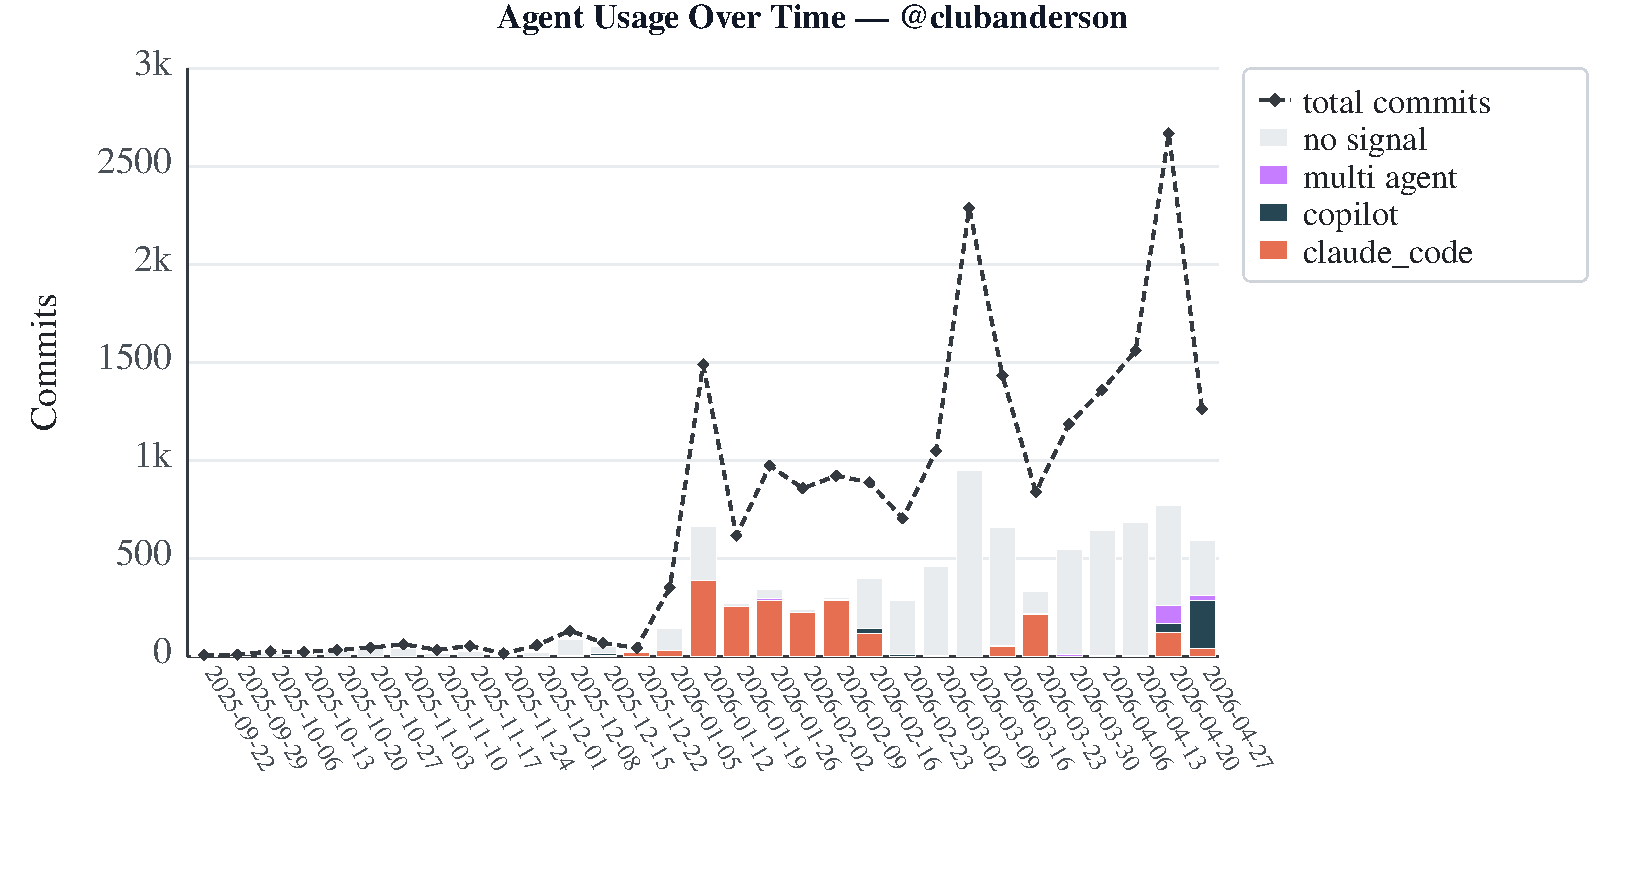
\includegraphics[width=\linewidth]{figures/rq2/rq2-agent-use-clubanderson.pdf}
  \caption{clubanderson}
  \label{fig:rq2-clubanderson}
\end{subfigure}

\begin{subfigure}{0.47\textwidth}
  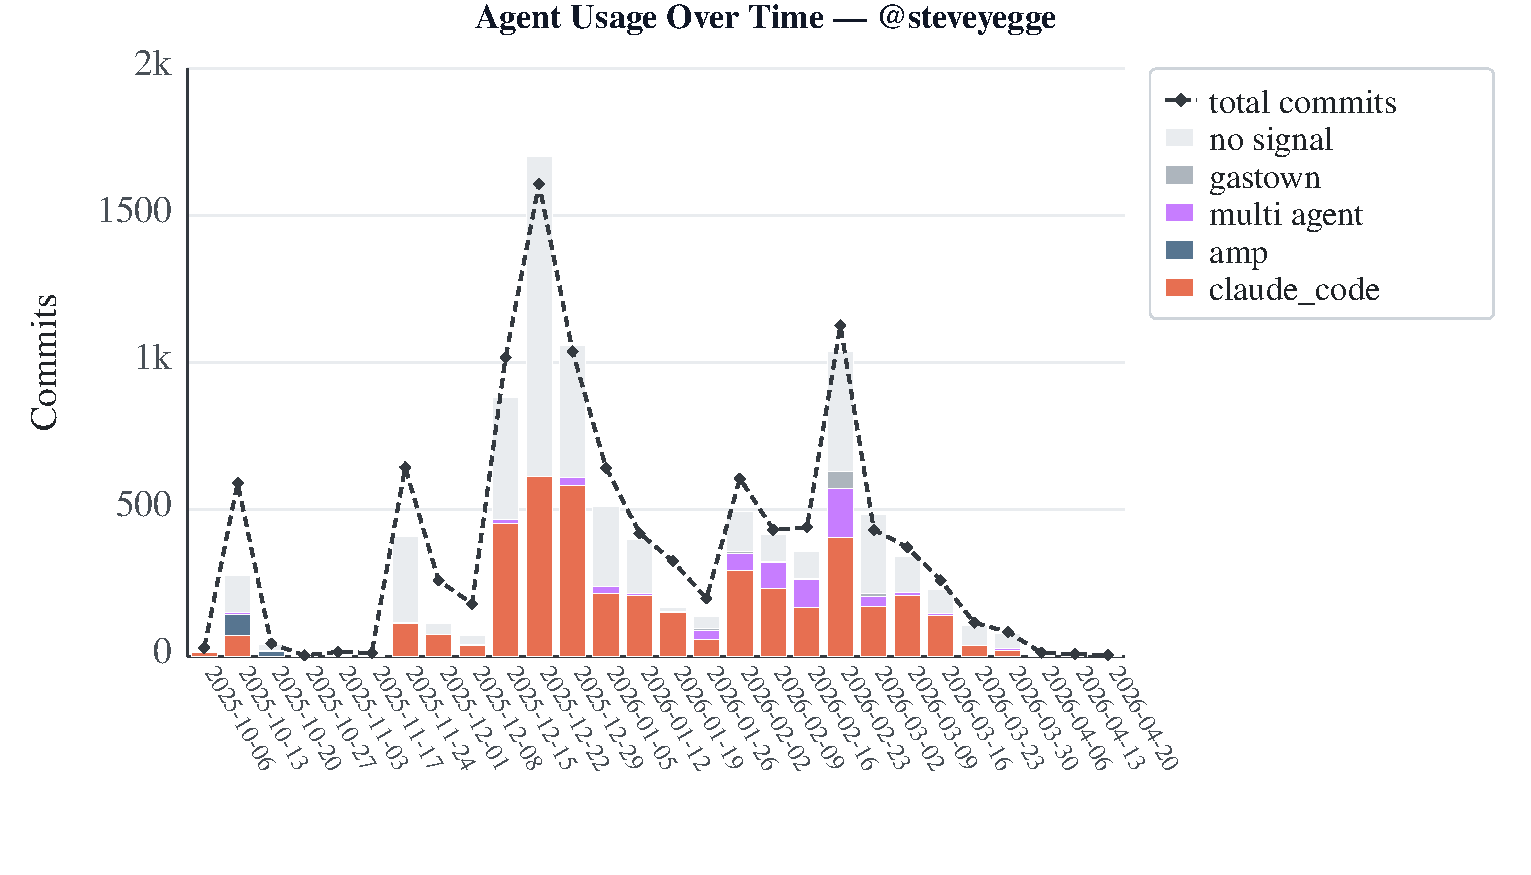
\includegraphics[width=\linewidth]{figures/rq2/rq2-agent-use-steveyegge.pdf}
  \caption{steveyegge}
  \label{fig:rq2-steveyegge}
\end{subfigure}\hfill
\begin{subfigure}{0.47\textwidth}
  
\includegraphics[width=\linewidth]{figures/rq2/rq2-agent-use-teamchong.pdf}
  \caption{teamchong}
  \label{fig:rq2-teamchong}
\end{subfigure}

\begin{subfigure}{0.47\textwidth}
  
\includegraphics[width=\linewidth]{figures/rq2/rq2-agent-use-steipete.pdf}
  \caption{steipete}
  \label{fig:rq2-steipete}
\end{subfigure}\hfill
\begin{subfigure}{0.47\textwidth}
  
\includegraphics[width=\linewidth]{figures/rq2/rq2-agent-use-ruvnet.pdf}
  \caption{ruvnet}
  \label{fig:rq2-ruvnet}
\end{subfigure}

\begin{subfigure}{0.47\textwidth}
  
\includegraphics[width=\linewidth]{figures/rq2/rq2-agent-use-obra.pdf}
  \caption{obra}
  \label{fig:rq2-obra}
\end{subfigure}\hfill
\begin{subfigure}{0.47\textwidth}
  
\includegraphics[width=\linewidth]{figures/rq2/rq2-agent-use-Dicklesworthstone.pdf}
  \caption{Dicklesworthstone}
  \label{fig:rq2-Dicklesworthstone}
\end{subfigure}

\begin{subfigure}{0.47\textwidth}
  
\includegraphics[width=\linewidth]{figures/rq2/rq2-agent-use-philipp-spiess.pdf}
  \caption{philipp-spiess}
  \label{fig:rq2-philipp-spiess}
\end{subfigure}\hfill
\begin{subfigure}{0.47\textwidth}
  \caption*{}
\end{subfigure}
\caption{Agent usage over time for each developer. Stacked bars show the distribution of detected agent harnesses per week. Solid and dashed lines show total and sampled commit counts respectively.}
\label{fig:rq2-agent-use}
\end{figure*}

\begin{figure*}[t]
\centering
\begin{subfigure}{0.47\textwidth}
  
\includegraphics[width=\linewidth]{figures/rq2/commit-types-agent-codex.pdf}
  \caption{Codex}
  \label{fig:rq2-codex}
\end{subfigure}\hfill
\begin{subfigure}{0.23\textwidth}
  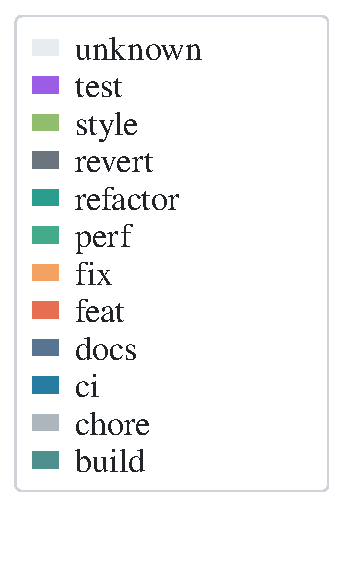
\includegraphics[width=\linewidth]{figures/rq2/commit-types-legend.pdf}
  \caption{Legend}
  \label{fig:rq2-commit-types-legend}
\end{subfigure}

\begin{subfigure}{0.47\textwidth}
  
\includegraphics[width=\linewidth]{figures/rq2/commit-types-agent-copilot.pdf}
  \caption{Copilot}
  \label{fig:rq2-copilot}
\end{subfigure}\hfill
\begin{subfigure}{0.47\textwidth}
  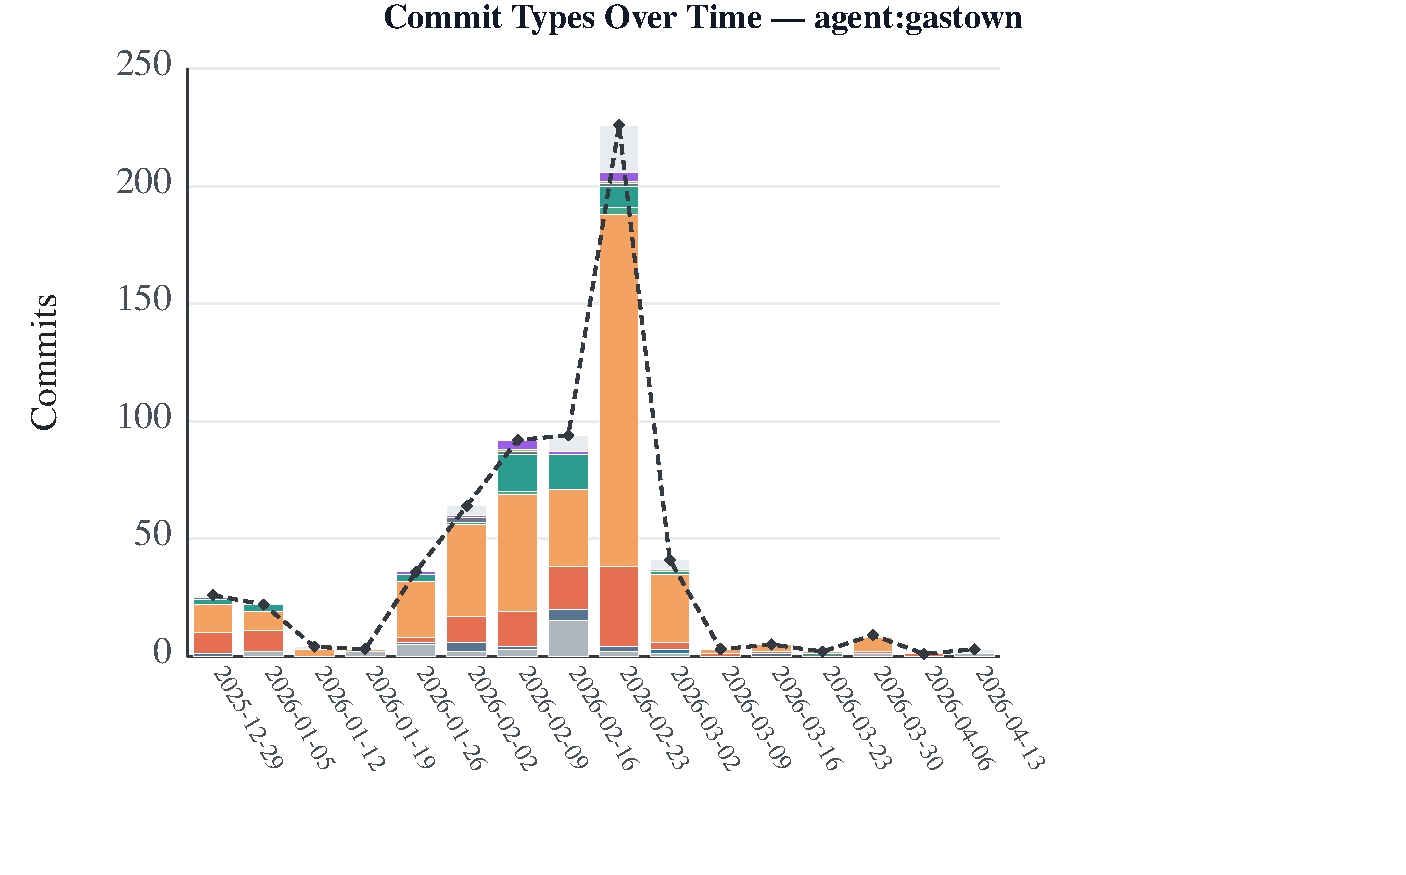
\includegraphics[width=\linewidth]{figures/rq2/commit-types-agent-gastown.pdf}
  \caption{Gastown}
  \label{fig:rq2-gastown}
\end{subfigure}

\begin{subfigure}{0.47\textwidth}
  
\includegraphics[width=\linewidth]{figures/rq2/commit-types-agent-opencode.pdf}
  \caption{OpenCode}
  \label{fig:rq2-opencode}
\end{subfigure}\hfill
\begin{subfigure}{0.47\textwidth}
  
\includegraphics[width=\linewidth]{figures/rq2/commit-types-agent-cursor.pdf}
  \caption{Cursor}
  \label{fig:rq2-cursor}
\end{subfigure}

\begin{subfigure}{0.47\textwidth}
  
\includegraphics[width=\linewidth]{figures/rq2/commit-types-agent-claude_code.pdf}
  \caption{Claude Code}
  \label{fig:rq2-claude_code}
\end{subfigure}\hfill
\begin{subfigure}{0.47\textwidth}
  
\includegraphics[width=\linewidth]{figures/rq2/commit-types-agent-amp.pdf}
  \caption{Amp}
  \label{fig:rq2-amp}
\end{subfigure}
\caption{Distribution of commit types per agent harness. Each chart shows the proportion of conventional commit types (e.g., feat, fix, refactor) for commits attributed to a specific harness.}
\label{fig:rq2-commit-types-per-agent}
\end{figure*}



\subsection*{RQ3 — Repository Switching Behavior (@Martin and team)}
\emph{How do hyperactive AI-augmented developers switch across repositories?}

Prior work suggests that developers seek to multitask across projects, but that excessive multitasking may negatively affect productivity~\cite{Vasilescu2016sky}. While most developers contribute to multiple repositories at least occasionally, sustained day-to-day multitasking across repositories remains comparatively uncommon.
%
AI coding agents may alter these dynamics by autonomously executing implementation tasks after instruction, allowing developers to work on other repositories while the agent continues operating. Combined with higher-level prompting interfaces that require less continuous repository-specific interaction, this may reduce the practical costs of switching between repositories and enable more fluid multi-repository workflows.
%
A repository switch is defined as two consecutive commits targeting different repositories.
%
We analyze repository-switching behavior using three complementary measures:
(i) the number of actively maintained repositories per developer-week, defined as repositories receiving at least two commits within the week based on prior work~\cite{Damota2022deep}; higher values may indicate broader concurrent activity enabled by lower context-switching costs; %make it a week
(ii) repository concentration measured using the Gini coefficient, where values near 1 indicate activity concentrated in a small number of repositories and lower values indicate more evenly distributed work; and %measured over a week
(iii) repository switch counts at the day and session levels, where unusually high values may reflect highly fragmented or strongly parallelized development workflows. We segment activity into sessions using a 30-minute inactivity threshold, per prior work on developer activity sessionization~\cite{Mozannar2024when}.
%
We report these measures for each developer and compare them with pre-agent
baselines (cf. Section~\ref{sec:baseline}).

\subsection*{RQ4 — Commit Quality (@Thomas/Romain and team)}
\emph{What is the quality of the commits and code produced by the considered hyperactive AI-augmented developers?}

High commit volumes can strain human oversight and may affect the structure and
maintainability of the resulting code. He~et~al.~\cite{he2025speed} report that
AI-assisted contributions can buy short-term velocity at the cost of long-term
maintainability and accumulating complexity, and Xu~et~al.~\cite{Xu2026} document
measurable LLM-induced shifts in coding style, complexity, and maintainability
across thousands of repositories.
We measure commit quality at the \emph{commit} and \emph{code} levels.

\paragraph{Commit-level cleanliness.}
At the commit level, we treat a commit as a unit of change and assess whether it is appropriately sized and focused on a single concern.
We characterize each commit along three observable dimensions: its \emph{breadth} (the number of files touched and the number of distinct top-level directories they span) and its \emph{size} (the number of lines added and removed, \ie the churn).

Churn weighs every changed line equally, whatever the line belongs to. To
qualify it, we assign each changed file to exactly one of six categories from
its path and extension: \emph{code} (source files in any of 48 language
extensions), \emph{tests} (files under a test directory, or named as a test),
\emph{documentation} (Markdown, reStructuredText, plain text, and files
under \texttt{docs/} or \texttt{examples/}), \emph{configuration} (YAML, TOML,
JSON, along with build, CI, and lockfile names), \emph{data} (fixtures,
snapshots, corpora, and tabular or binary data formats), and the residual
\emph{others} category.

\paragraph{Code-level quality.}
Commit-level signals describe how change is delivered but not the intrinsic quality of the code that results.
At the code level we therefore compute simple, language-agnostic structural metrics: total lines of code, function and method size, cyclomatic complexity, comment density, and the presence and quantity of tests; where tractable, we additionally consider cohesion and coupling proxies.
We compute these metrics on the post-commit state of the changed files and
track their evolution over the observation window.

\paragraph{ASAT-based quality.}
Finally, we conduct a coarser-grained analysis using automated static-analysis
tools (ASATs).
Prior work studies agent-influenced quality through such tools~\cite{he2025speed}, but running them per commit is intractable at our dataset's volume and granularity.
We snapshot a subset of representative projects at a fixed cadence (\eg once
per day) and run an ASAT (\eg SonarQube) on each snapshot. We report the
resulting quality measures and rule violations (code smells, reliability and
security issues, adherence to best practices) as a complementary, project-level
view.

% Operationalization: commit-level signals via \texttt{analyze-commit-quality.py} and
% \texttt{analyze-commits.py} (concern classification + Conventional Commits + clean/dirty
% flags), file-touch breadth via \texttt{visualize-file-touches.py}; code-level metrics and

%-----------------------------------------------------------------------
\section{Results}
\label{sec:results}

% All subsections are stubs; detailed findings will be filled in after data analysis scripts are run.
\subsection{RQ1: Temporal Activity Patterns}

Figure~\ref{fig:rq1-months} shows the monthly commit counts of each developer.

\textbf{Monthly activity rises sharply and then declines.} Overall, developers
follow a similar trajectory, characterized by a sharp increase in commit
activity followed by a rapid decline. This is clearly visible for \texttt{mavan} and \texttt{steveyegge}.


\textbf{Three developers resume growth near the end of the observation period.}
Despite a drop between January and February 2026 for \texttt{clubanderson} and
\texttt{steipete}, and between January and March 2026 for \texttt{ruvnet}, these
three developers are the only ones showing a subsequent increase in commit
activity towards the end of the observation period, \ie in April 2026.


\textbf{Dicklesworthstone has the highest commit volume.} Only two of the nine developers, \ie
\texttt{mavan} and \texttt{philipp-spiess}, never surpass 1,000 monthly commits.
\texttt{Dicklesworthstone} shows the highest level of activity among the studied
developers, reaching a peak of 19,188 commits in April 2026 and accumulating
71,420 commits throughout the observation period. He is a paradigmatic hyperactive AI developer.

\begin{figure*}[t]
  \centering
  \begin{subfigure}{0.3\textwidth}
    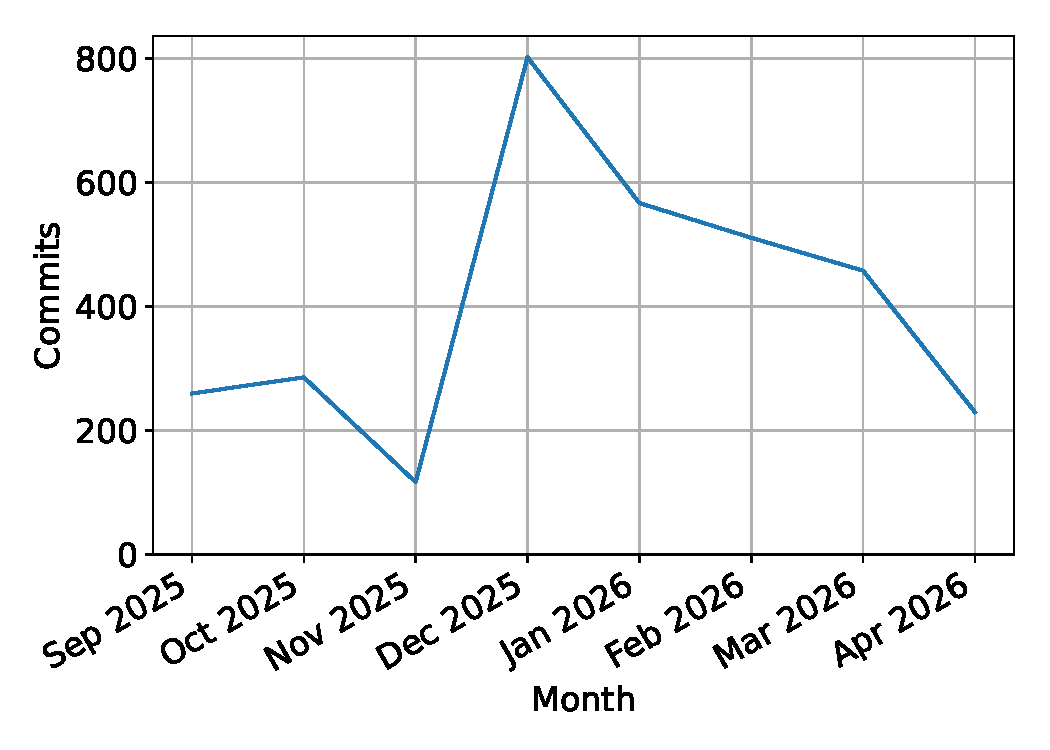
\includegraphics[width=\linewidth]{../figures/mavam-timeframe.pdf}
    \caption{mavam}
    \label{fig:rq1-months-mavam}
  \end{subfigure}
  %
  \begin{subfigure}{0.3\textwidth}
    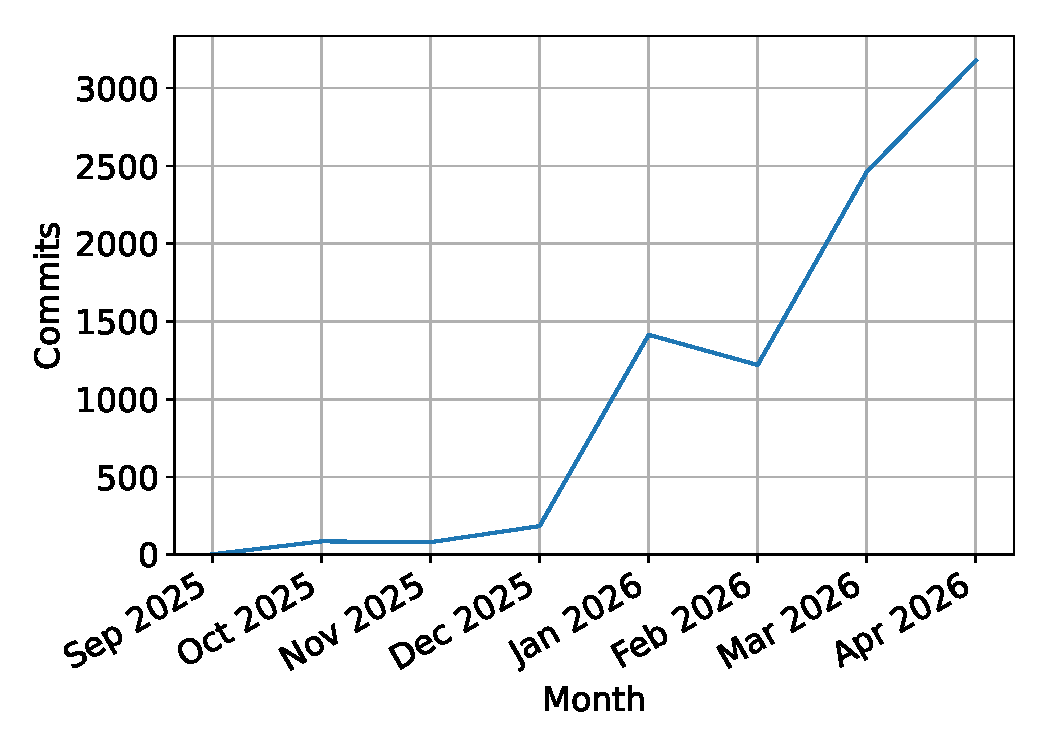
\includegraphics[width=\linewidth]{../figures/clubanderson-timeframe.pdf}
    \caption{clubanderson}
    \label{fig:rq1-months-clubanderson}
  \end{subfigure}
  %
  \begin{subfigure}{0.3\textwidth}
    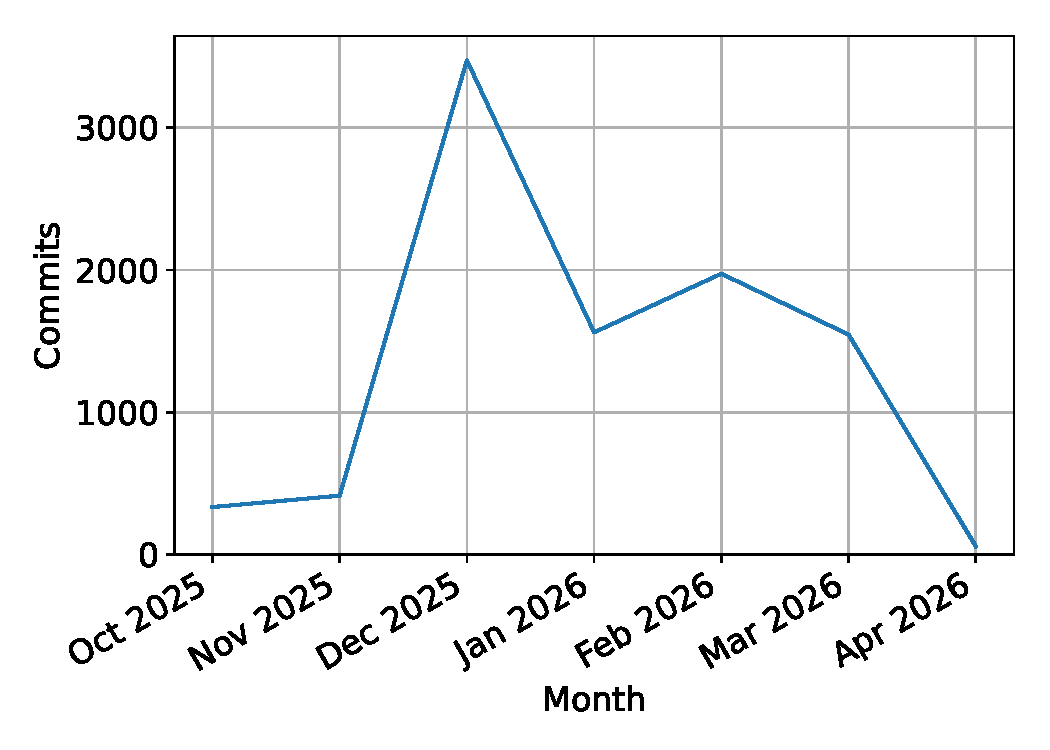
\includegraphics[width=\linewidth]{../figures/steveyegge-timeframe.pdf}
    \caption{steveyegge}
    \label{fig:rq1-months-steveyegge}
  \end{subfigure}

  \begin{subfigure}{0.3\textwidth}
    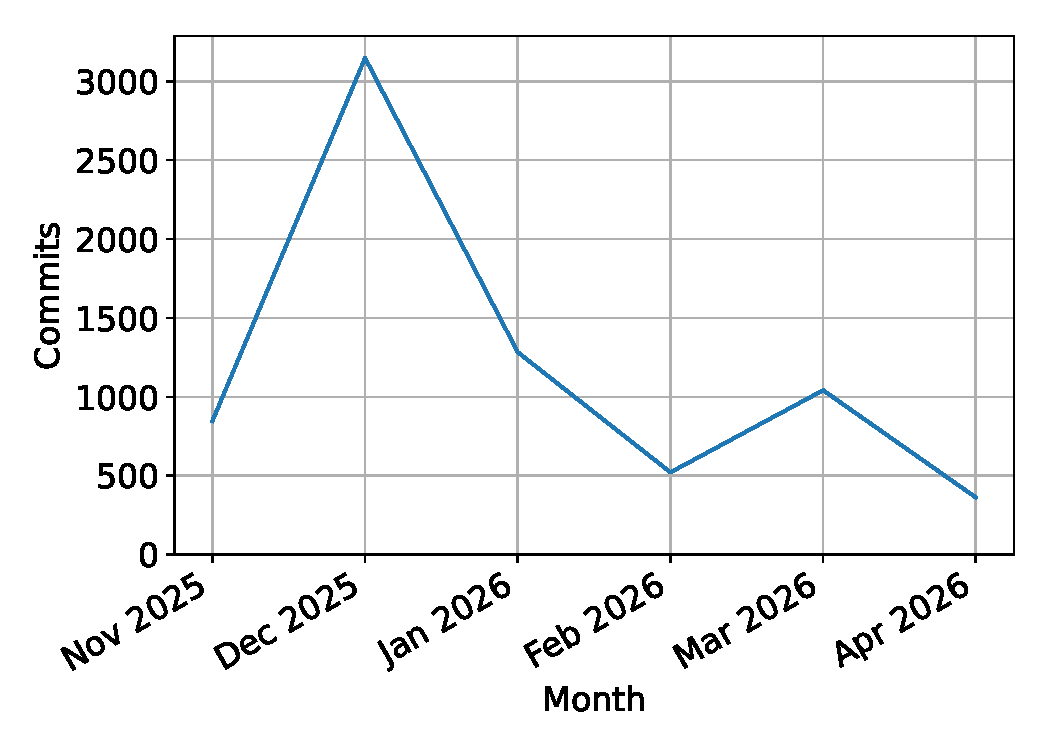
\includegraphics[width=\linewidth]{../figures/teamchong-timeframe.pdf}
    \caption{teamchong}
    \label{fig:rq1-months-teamchong}
  \end{subfigure}
  %
  \begin{subfigure}{0.3\textwidth}
    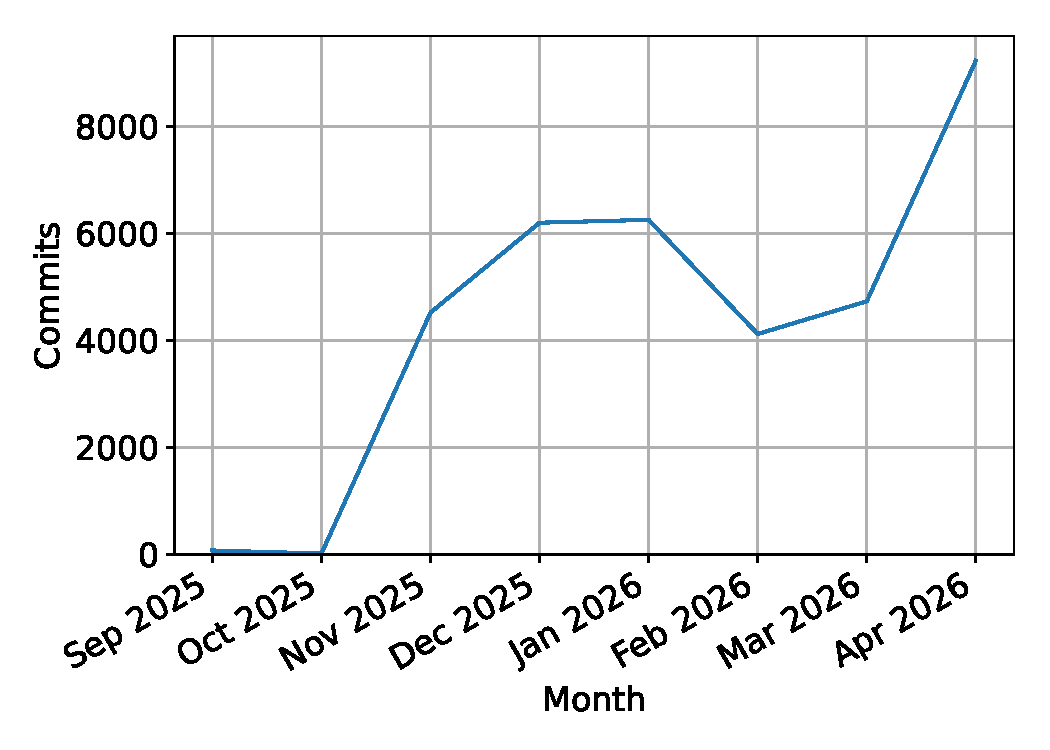
\includegraphics[width=\linewidth]{../figures/steipete-timeframe.pdf}
    \caption{steipete}
    \label{fig:rq1-months-steipete}
  \end{subfigure}
  %
  \begin{subfigure}{0.3\textwidth}
    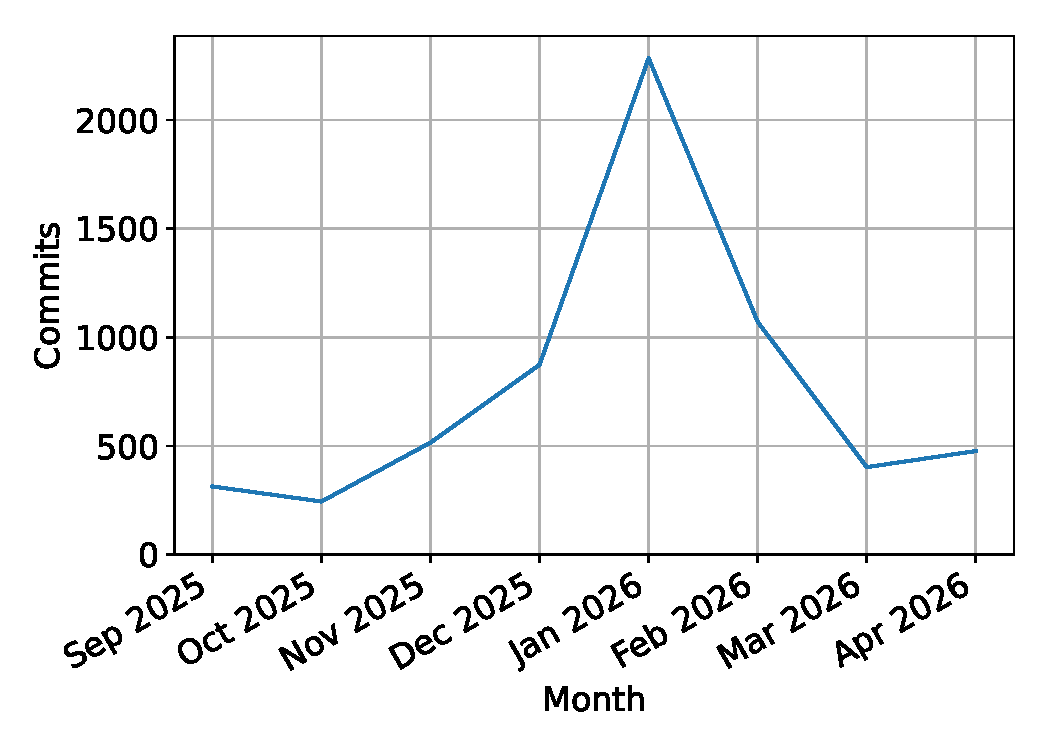
\includegraphics[width=\linewidth]{../figures/ruvnet-timeframe.pdf}
    \caption{ruvnet}
    \label{fig:rq1-months-ruvnet}
  \end{subfigure}

  \begin{subfigure}{0.3\textwidth}
    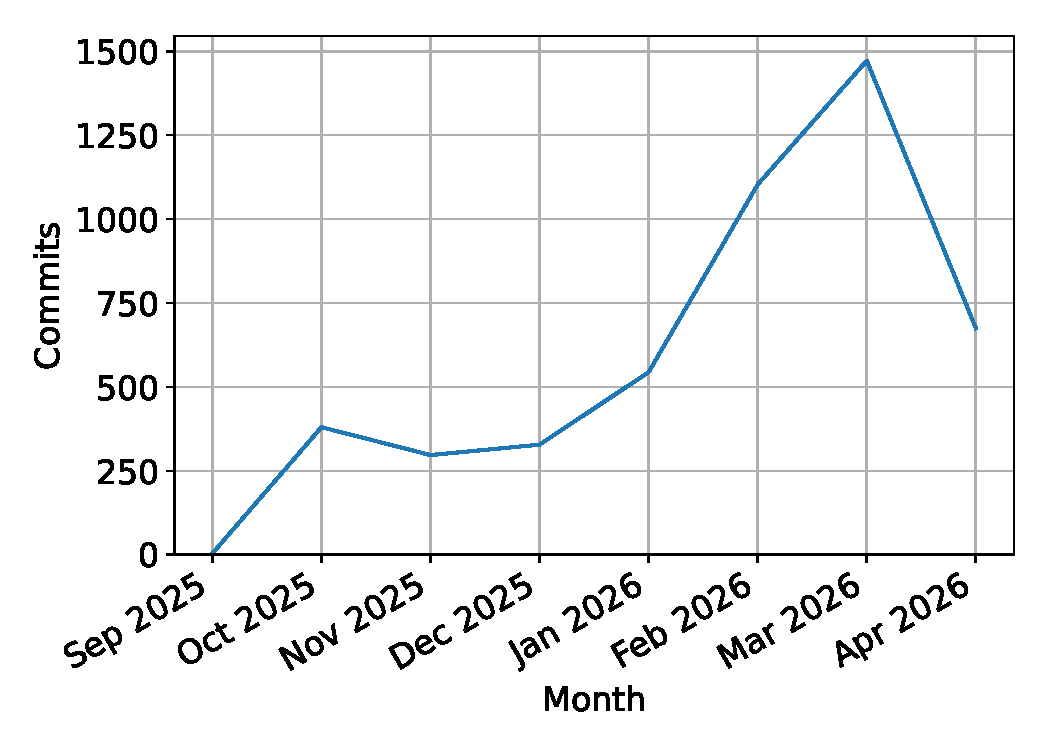
\includegraphics[width=\linewidth]{../figures/obra-timeframe.pdf}
    \caption{obra}
    \label{fig:rq1-months-obra}
  \end{subfigure}
  %
  \begin{subfigure}{0.3\textwidth}
    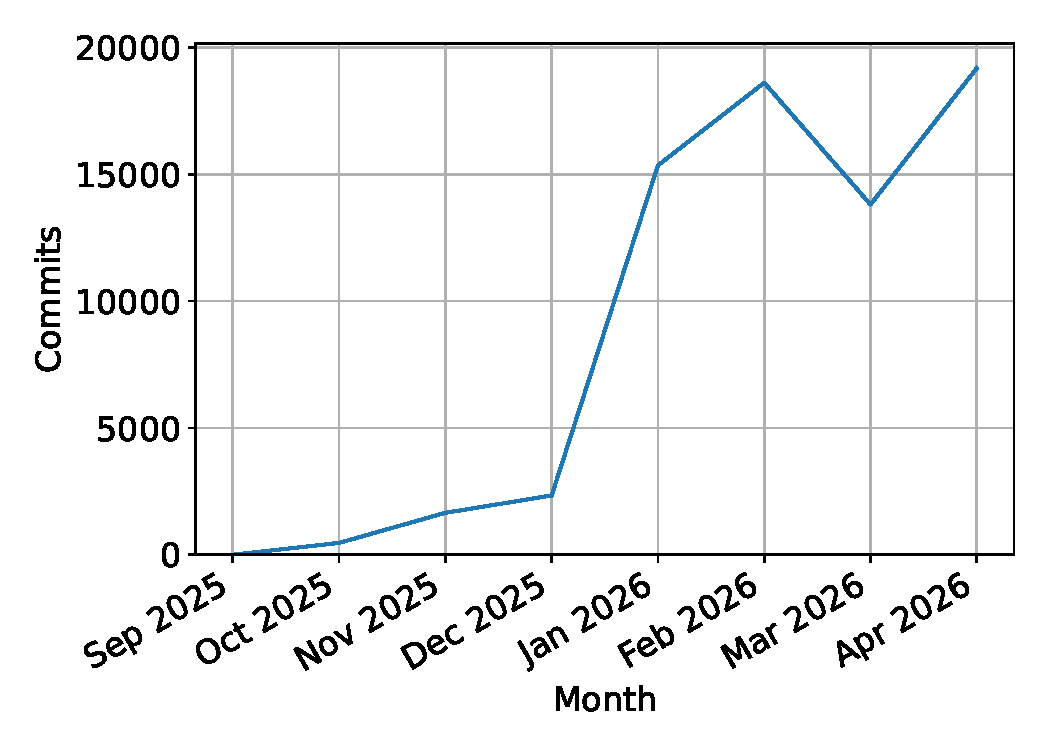
\includegraphics[width=\linewidth]{../figures/Dicklesworthstone-timeframe.pdf}
    \caption{Dicklesworthstone}
    \label{fig:rq1-months-Dicklesworthstone}
  \end{subfigure}
  %
  \begin{subfigure}{0.3\textwidth}
    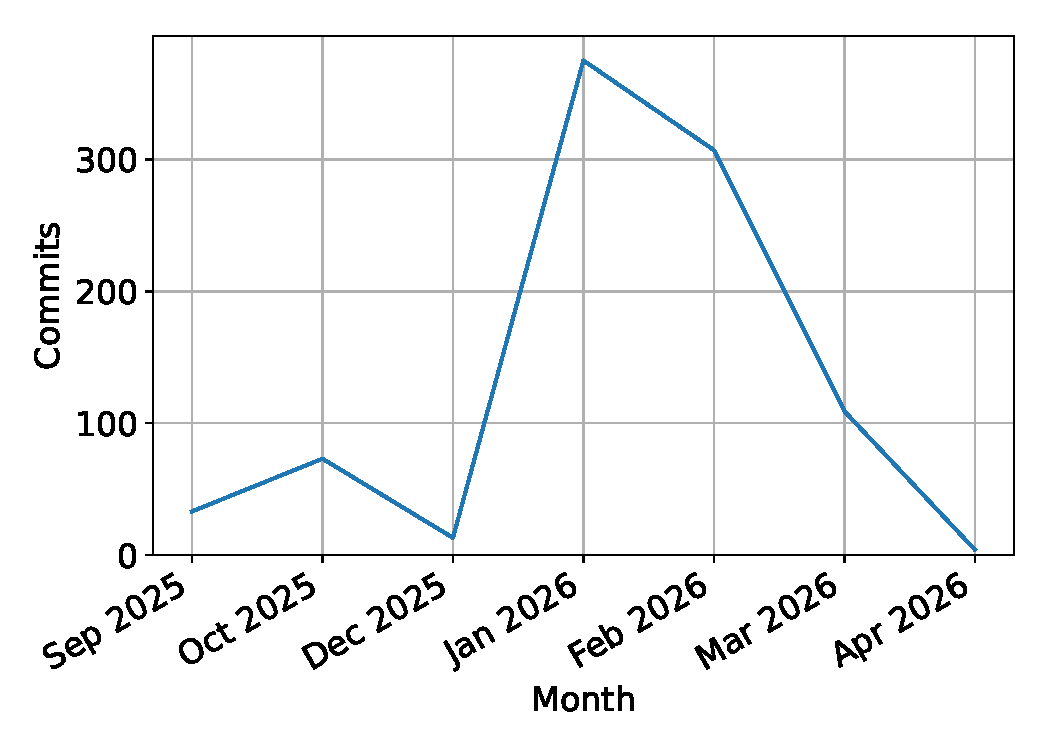
\includegraphics[width=\linewidth]{../figures/philipp-spiess-timeframe.pdf}
    \caption{philipp-spiess}
    \label{fig:rq1-months-philipp-spiess}
  \end{subfigure}

  \caption{Aggregated commits produced for each developer per month across the
    studied timeframe.}
  \label{fig:rq1-months}
\end{figure*}

Figure~\ref{fig:rq1-weekdays} shows the temporal distribution of commits
produced per weekday.

\textbf{Weekly activity patterns vary across developers.} \texttt{Dicklesworthstone}
and \texttt{obra} reach their highest activity levels during weekends in certain
months (February and March, respectively), whereas others reach higher activity
levels on weekdays. The most active developer per week is 
\texttt{philipp-spiess} who surpassed more than 100 commits in a
single day.

\begin{figure*}[t]
  \centering
  \begin{subfigure}{0.3\textwidth}
    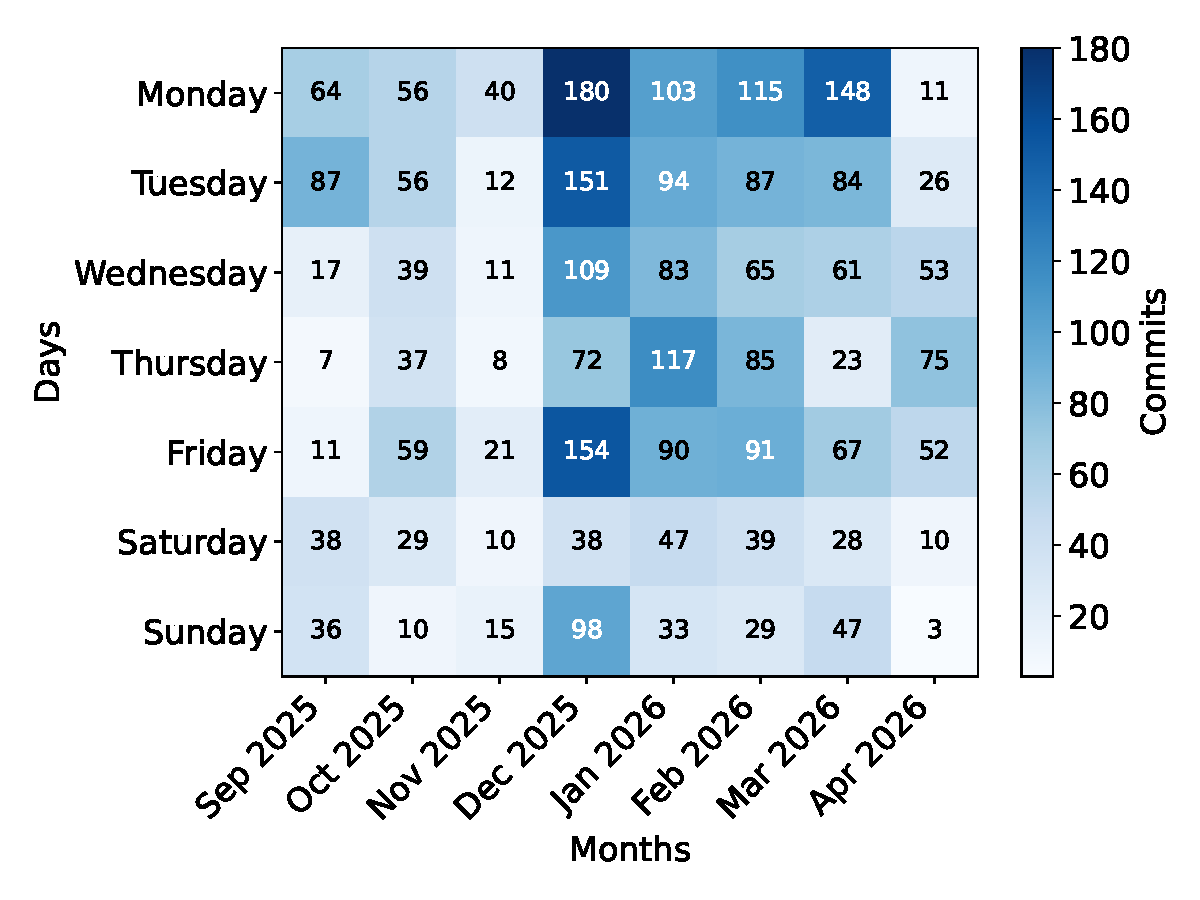
\includegraphics[width=\linewidth]{../figures/mavam-weekdays.pdf}
    \caption{mavam}
    \label{fig:rq1-weekdays-mavam}
  \end{subfigure}
  %
  \begin{subfigure}{0.3\textwidth}
    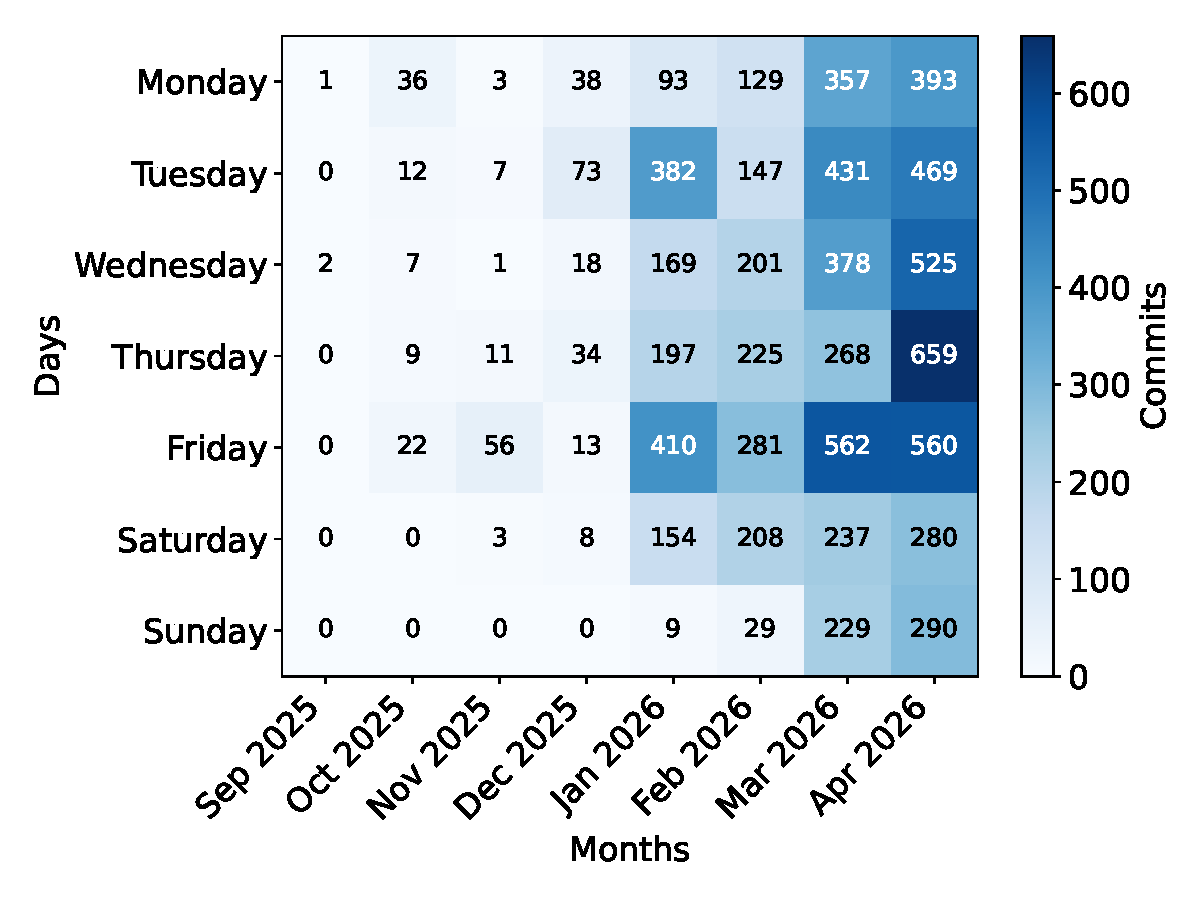
\includegraphics[width=\linewidth]{../figures/clubanderson-weekdays.pdf}
    \caption{clubanderson}
    \label{fig:rq1-weekdays-clubanderson}
  \end{subfigure}
  %
  \begin{subfigure}{0.3\textwidth}
    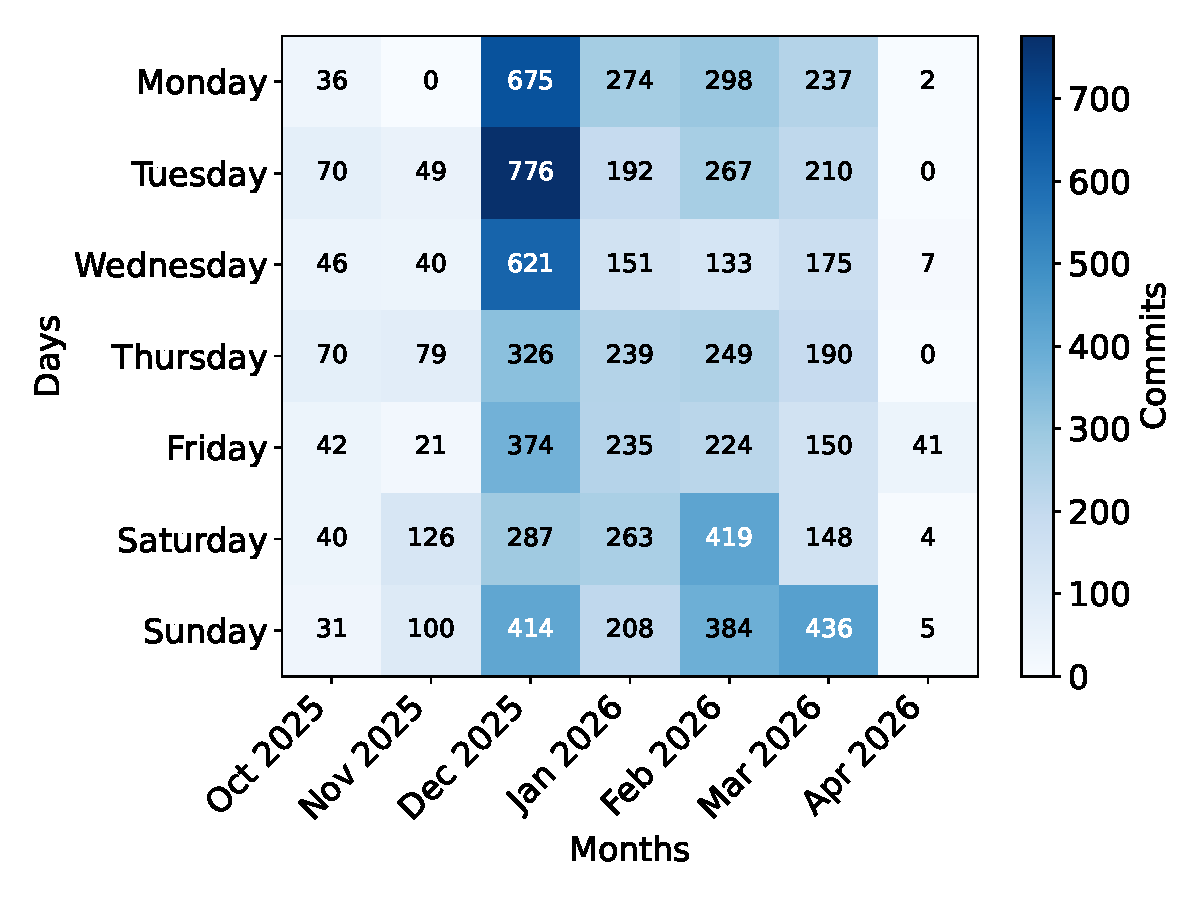
\includegraphics[width=\linewidth]{../figures/steveyegge-weekdays.pdf}
    \caption{steveyegge}
    \label{fig:rq1-weekdays-steveyegge}
  \end{subfigure}

  \begin{subfigure}{0.3\textwidth}
    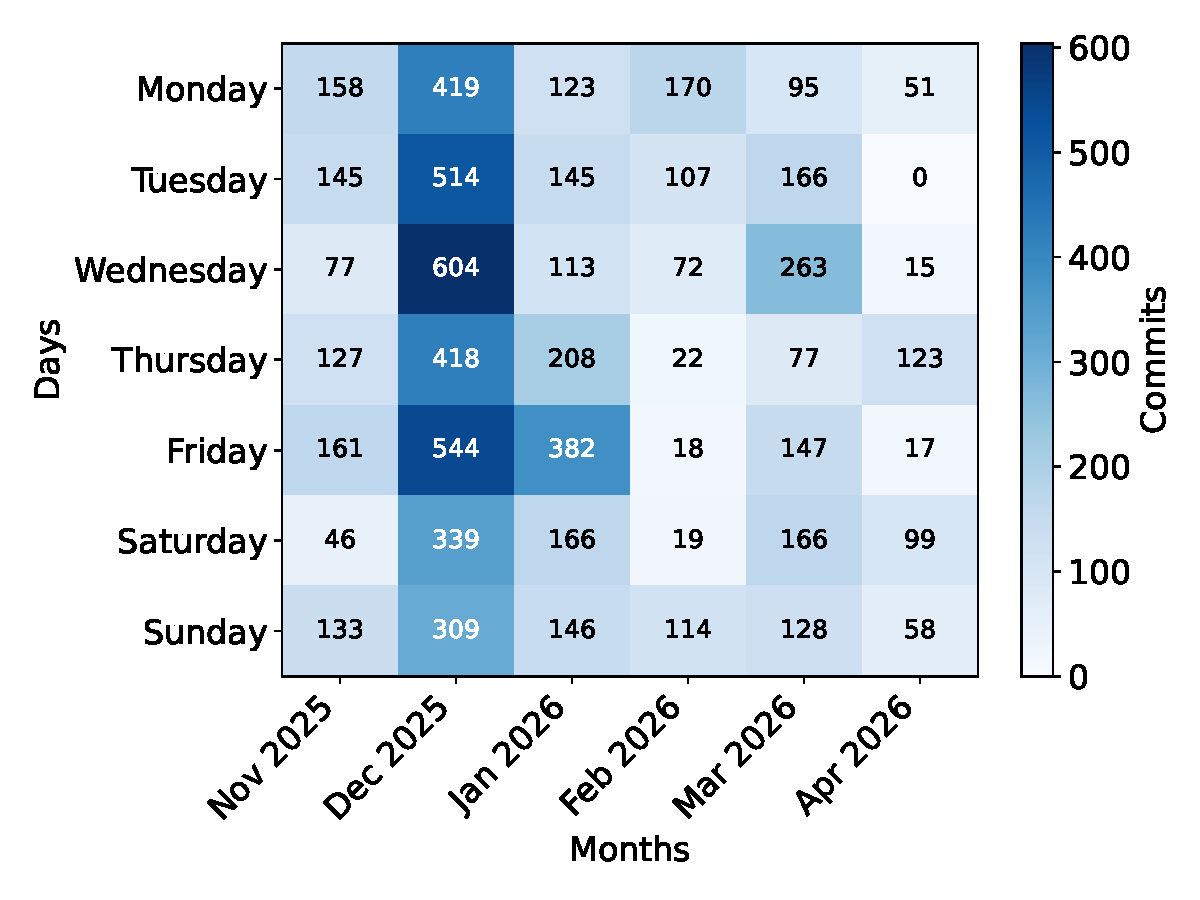
\includegraphics[width=\linewidth]{../figures/teamchong-weekdays.pdf}
    \caption{teamchong}
    \label{fig:rq1-weekdays-teamchong}
  \end{subfigure}
  %
  \begin{subfigure}{0.3\textwidth}
    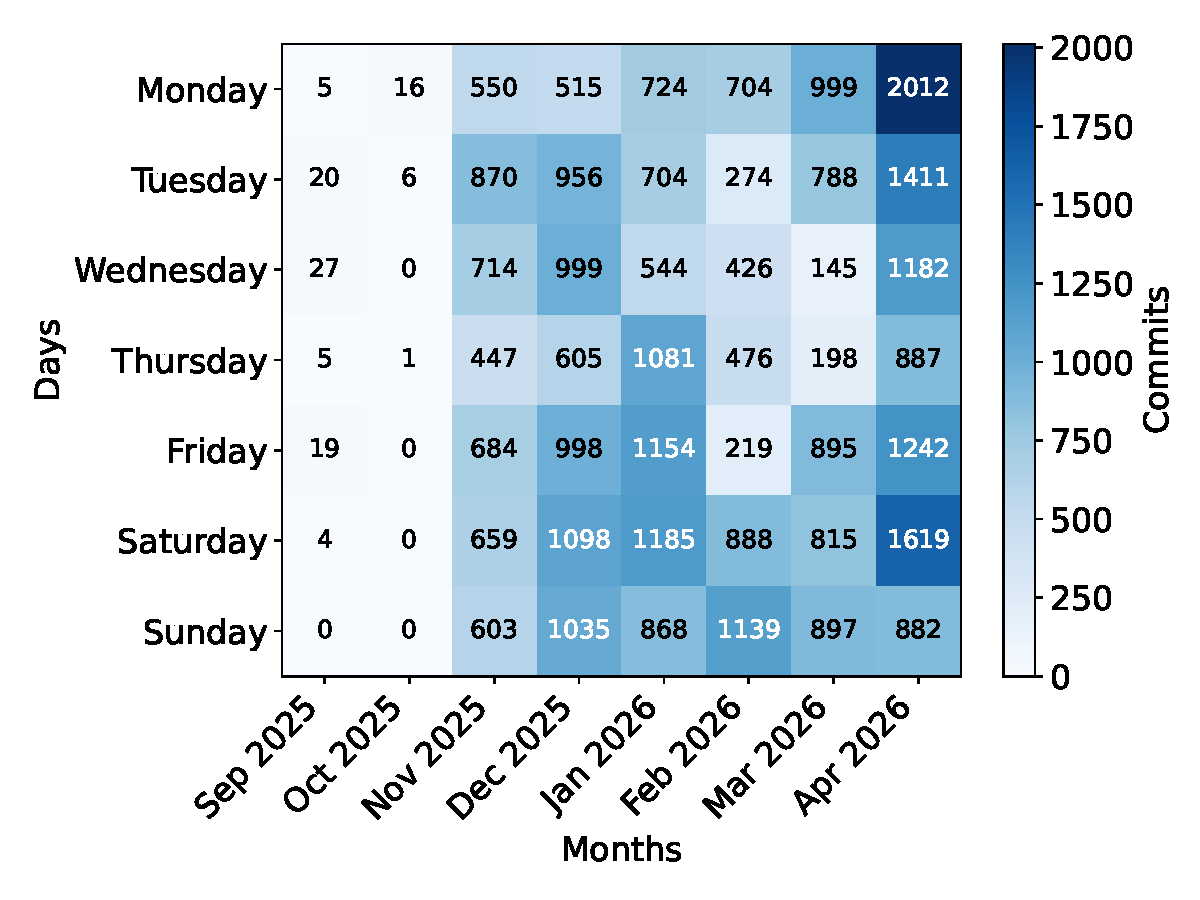
\includegraphics[width=\linewidth]{../figures/steipete-weekdays.pdf}
    \caption{steipete}
    \label{fig:rq1-weekdays-steipete}
  \end{subfigure}
  %
  \begin{subfigure}{0.3\textwidth}
    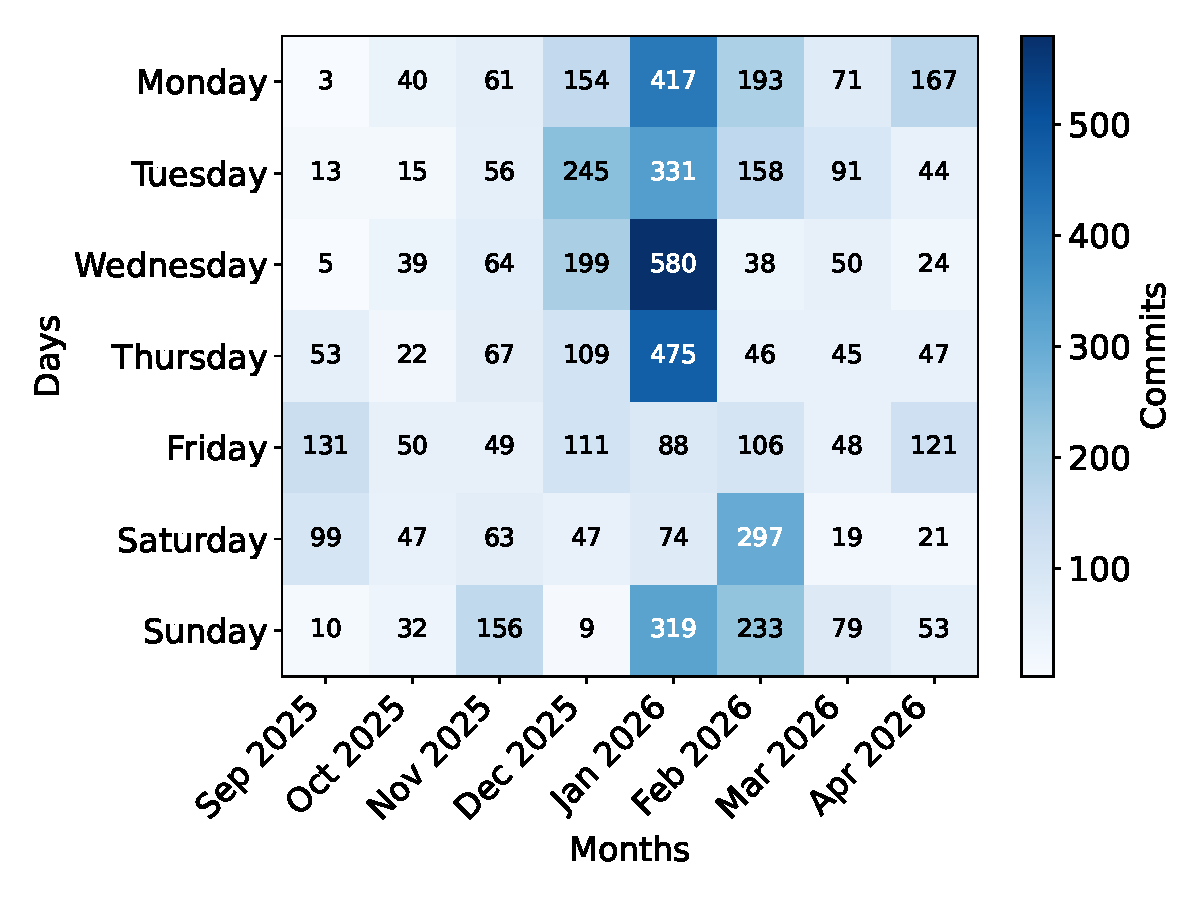
\includegraphics[width=\linewidth]{../figures/ruvnet-weekdays.pdf}
    \caption{ruvnet}
    \label{fig:rq1-weekdays-ruvnet}
  \end{subfigure}

  \begin{subfigure}{0.3\textwidth}
    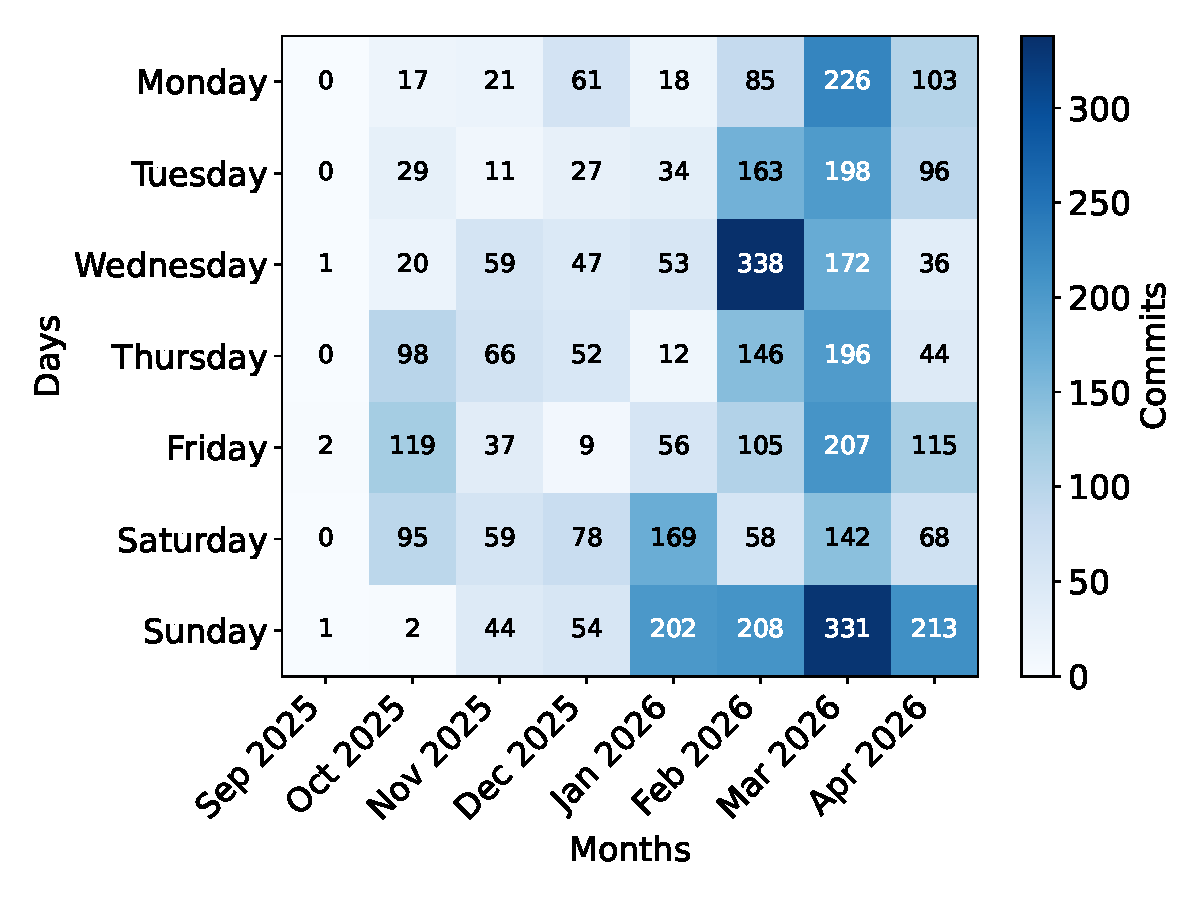
\includegraphics[width=\linewidth]{../figures/obra-weekdays.pdf}
    \caption{obra}
    \label{fig:rq1-weekdays-obra}
  \end{subfigure}
  %
  \begin{subfigure}{0.3\textwidth}
    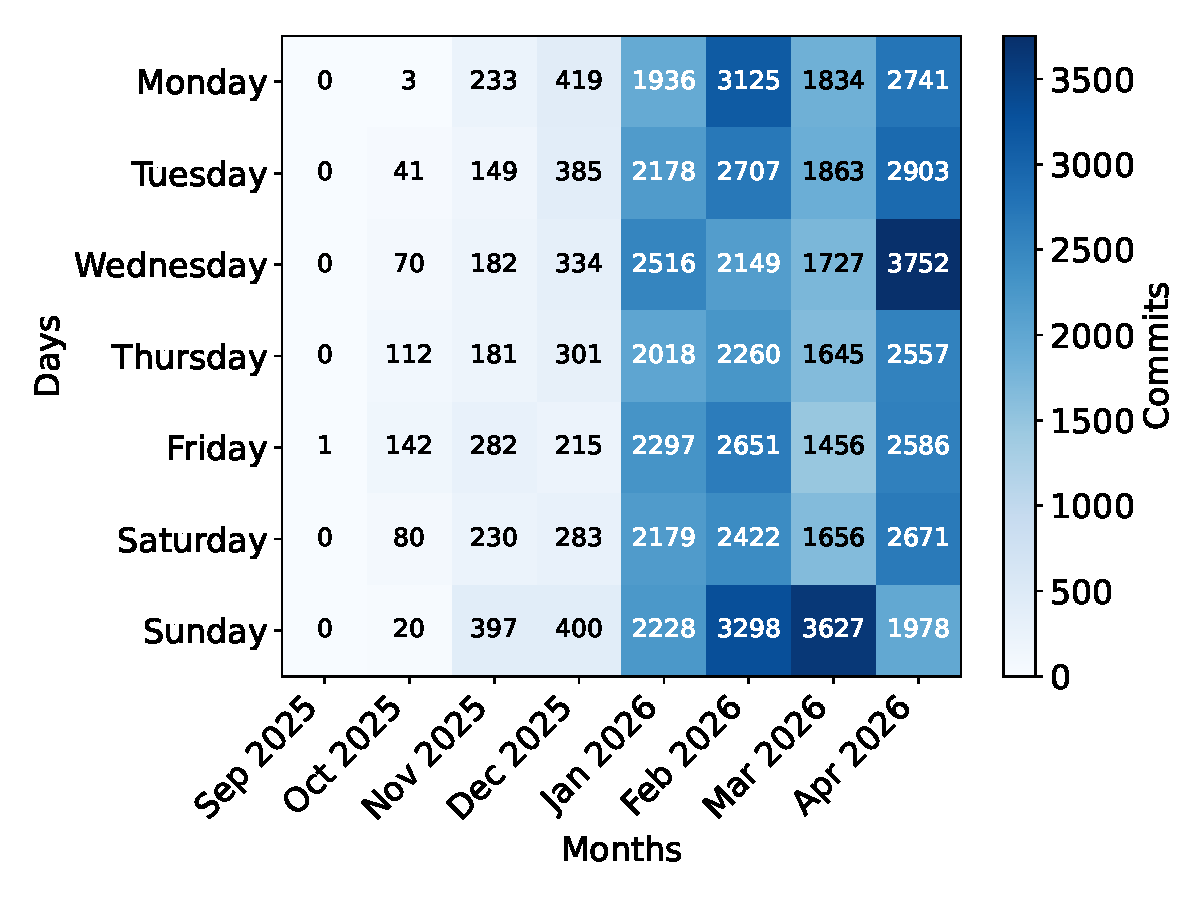
\includegraphics[width=\linewidth]{../figures/Dicklesworthstone-weekdays.pdf}
    \caption{Dicklesworthstone}
    \label{fig:rq1-weekdays-Dicklesworthstone}
  \end{subfigure}
  %
  \begin{subfigure}{0.3\textwidth}
    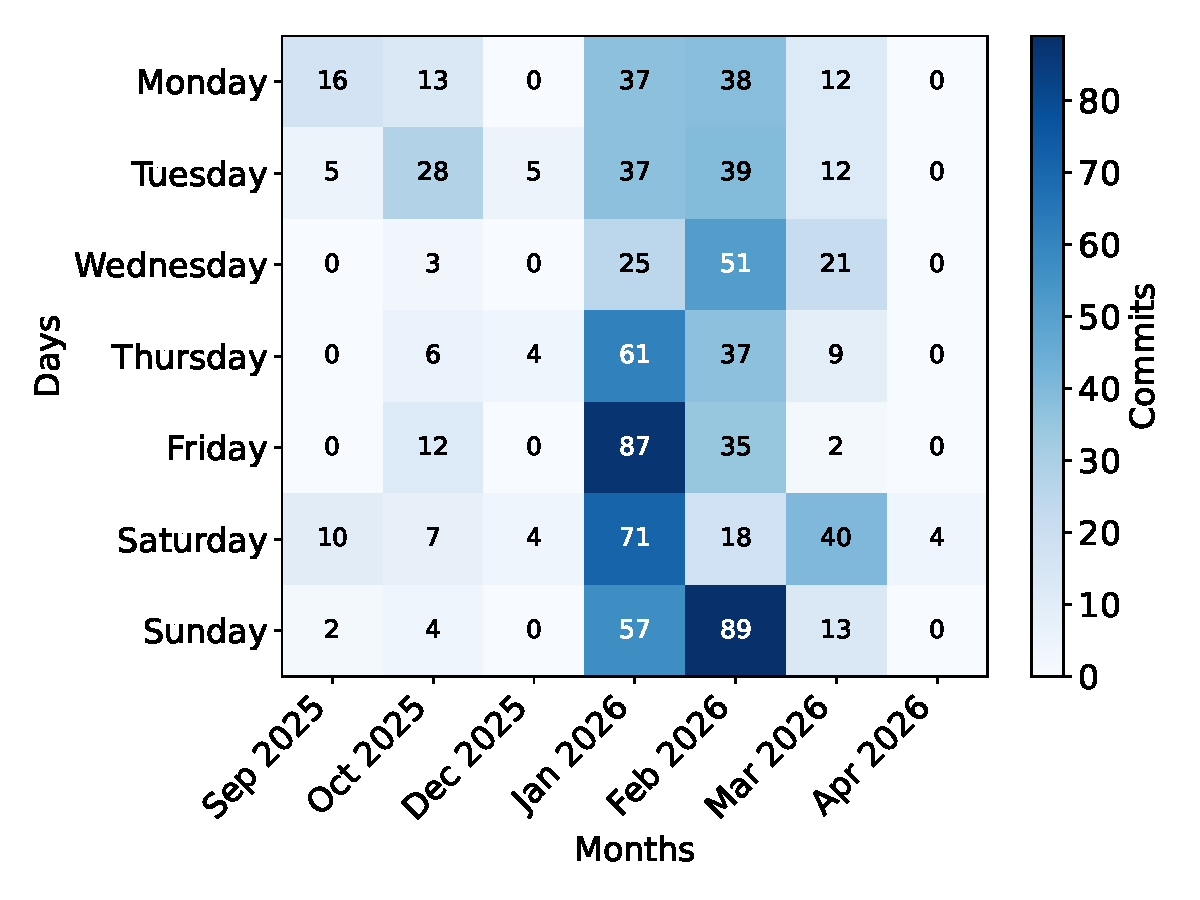
\includegraphics[width=\linewidth]{../figures/philipp-spiess-weekdays.pdf}
    \caption{philipp-spiess}
    \label{fig:rq1-weekdays-philipp-spiess}
  \end{subfigure}

  \caption{Heatmap showing the temporal distribution of commits produced per day across studied months.}
  \label{fig:rq1-weekdays}
\end{figure*}

\textbf{Intra-day activity follows a slowdown and speed-up pattern.}
Figure~\ref{fig:intra-day} shows the normalized hourly activity of developers,
for which the curves are LOWESS-smoothed.
%
We observe that developers follow two distinct phases. The first corresponds to
a slowdown phase during which activity gradually decreases, followed by a
speed-up phase.
%
Although commit activity is not plotted according to each developer's local time
zone, we assume that the first phase represent a rest period for developers, \ie
during which they do sleep; whereas the second phase represents an increase in
activity, \ie during which they do wake up.
%
As depicted in Figure~\ref{fig:rq1-intraday}, the slowdown phase lasts between
five to eight hours.
%
Despite these rest periods, developers continue to generate commits, suggesting
that AI agents continue performing tasks with limited developer intervention
during certain periods of time.

\begin{figure}
  \centering
  
\includegraphics[width=.85\linewidth]{figures/rq1/hourly}
  \caption{Lowess-smoothed curves of normalized aggregated commit count produced
    per hour for each developer across the studied timeframe.}
  \label{fig:intra-day}
\end{figure}

\begin{figure*}[t]
  \centering
  \begin{subfigure}{0.3\textwidth}
    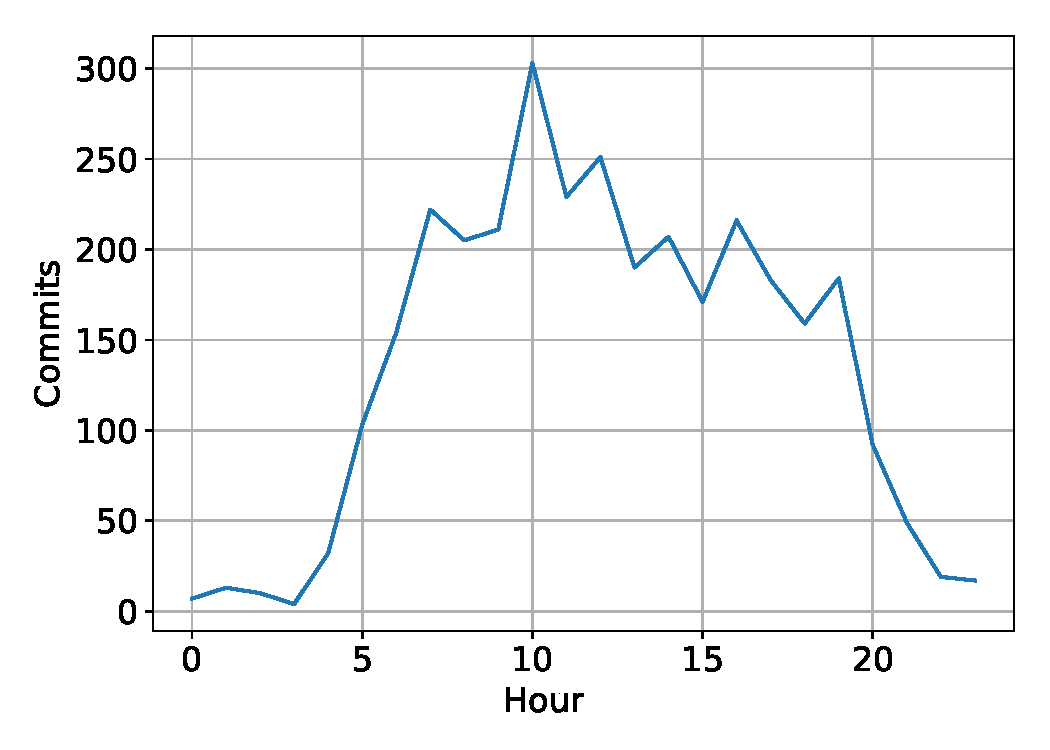
\includegraphics[width=\linewidth]{../figures/mavam-intraday.pdf}
    \caption{mavam}
    \label{fig:rq1-intraday-mavam}
  \end{subfigure}
  %
  \begin{subfigure}{0.3\textwidth}
    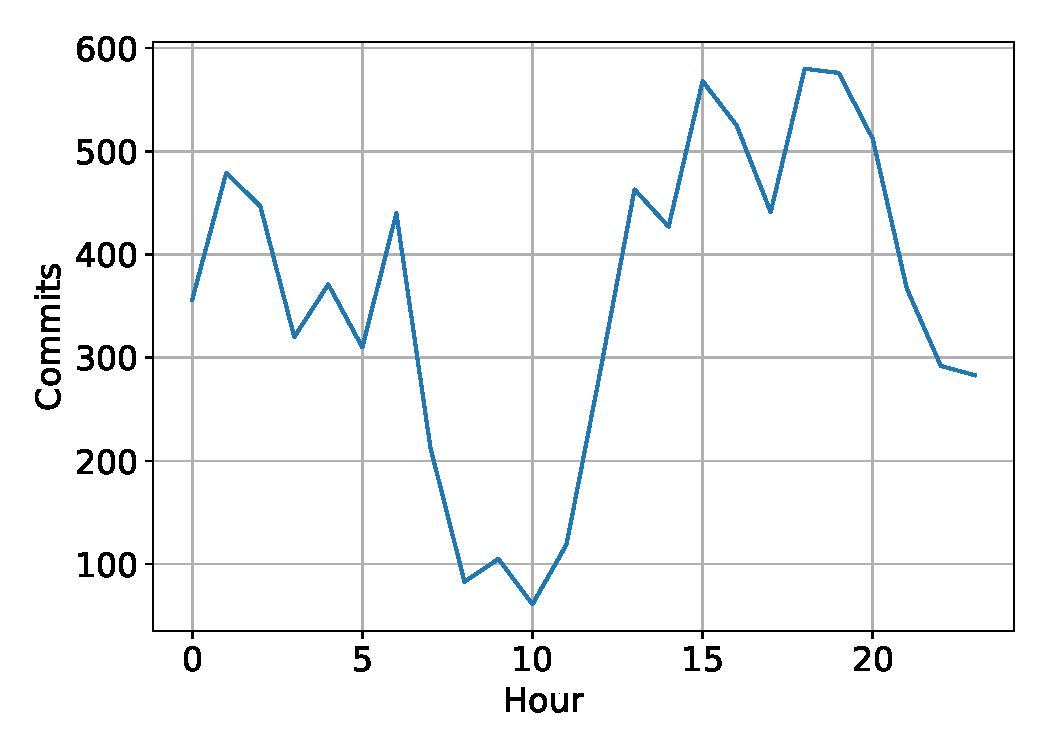
\includegraphics[width=\linewidth]{../figures/clubanderson-intraday.pdf}
    \caption{clubanderson}
    \label{fig:rq1-intraday-clubanderson}
  \end{subfigure}
  %
  \begin{subfigure}{0.3\textwidth}
    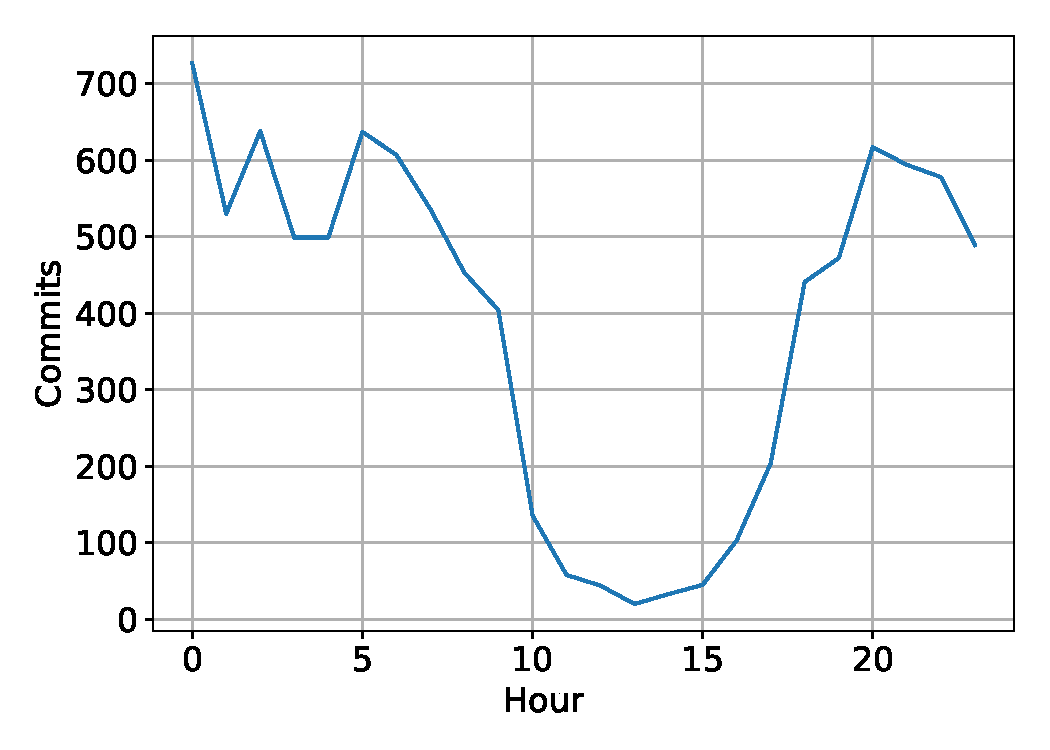
\includegraphics[width=\linewidth]{../figures/steveyegge-intraday.pdf}
    \caption{steveyegge}
    \label{fig:rq1-intraday-steveyegge}
  \end{subfigure}

  \begin{subfigure}{0.3\textwidth}
    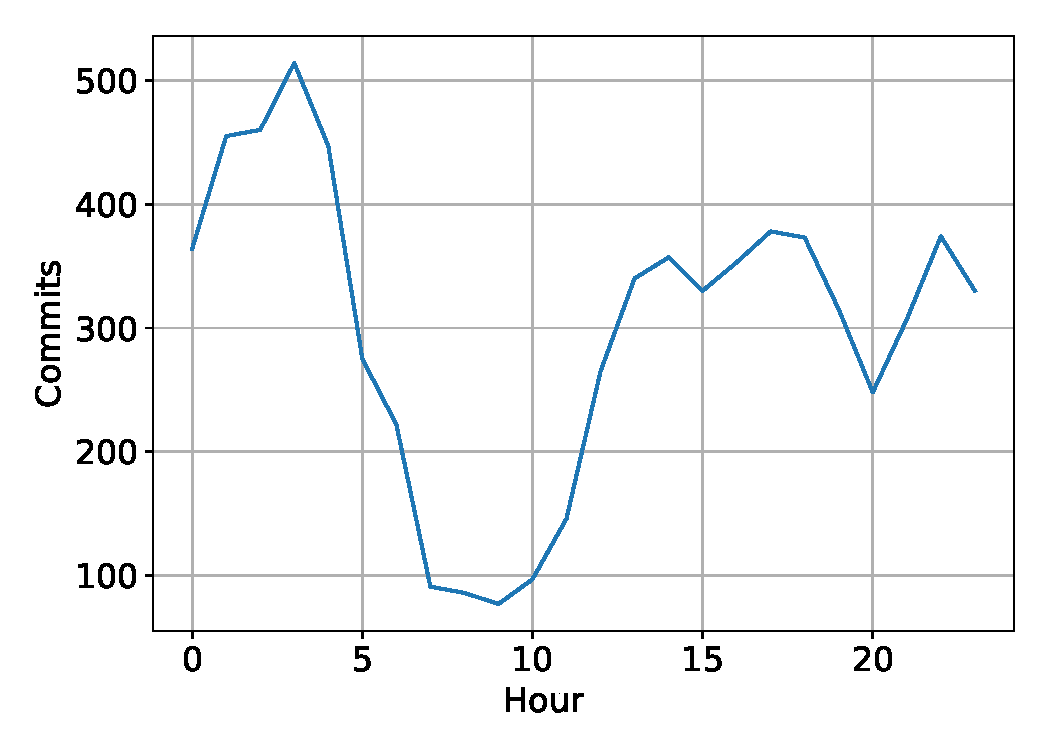
\includegraphics[width=\linewidth]{../figures/teamchong-intraday.pdf}
    \caption{teamchong}
    \label{fig:rq1-intraday-teamchong}
  \end{subfigure}
  %
  \begin{subfigure}{0.3\textwidth}
    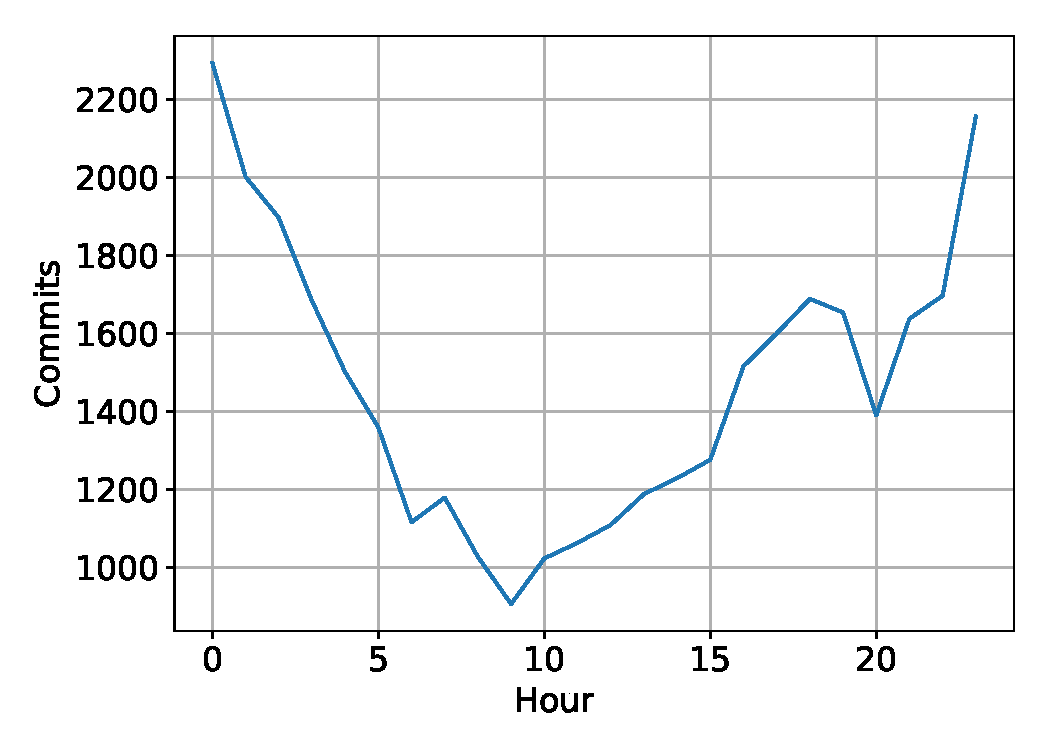
\includegraphics[width=\linewidth]{../figures/steipete-intraday.pdf}
    \caption{steipete}
    \label{fig:rq1-intraday-steipete}
  \end{subfigure}
  %
  \begin{subfigure}{0.3\textwidth}
    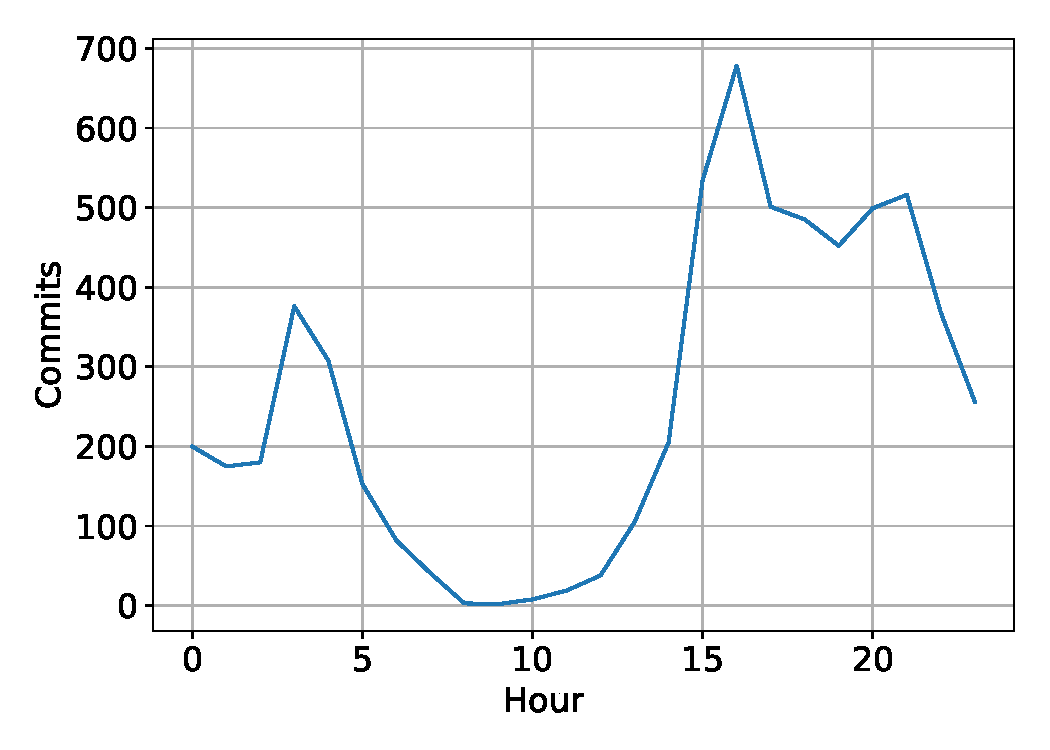
\includegraphics[width=\linewidth]{../figures/ruvnet-intraday.pdf}
    \caption{ruvnet}
    \label{fig:rq1-intraday-ruvnet}
  \end{subfigure}

  \begin{subfigure}{0.3\textwidth}
    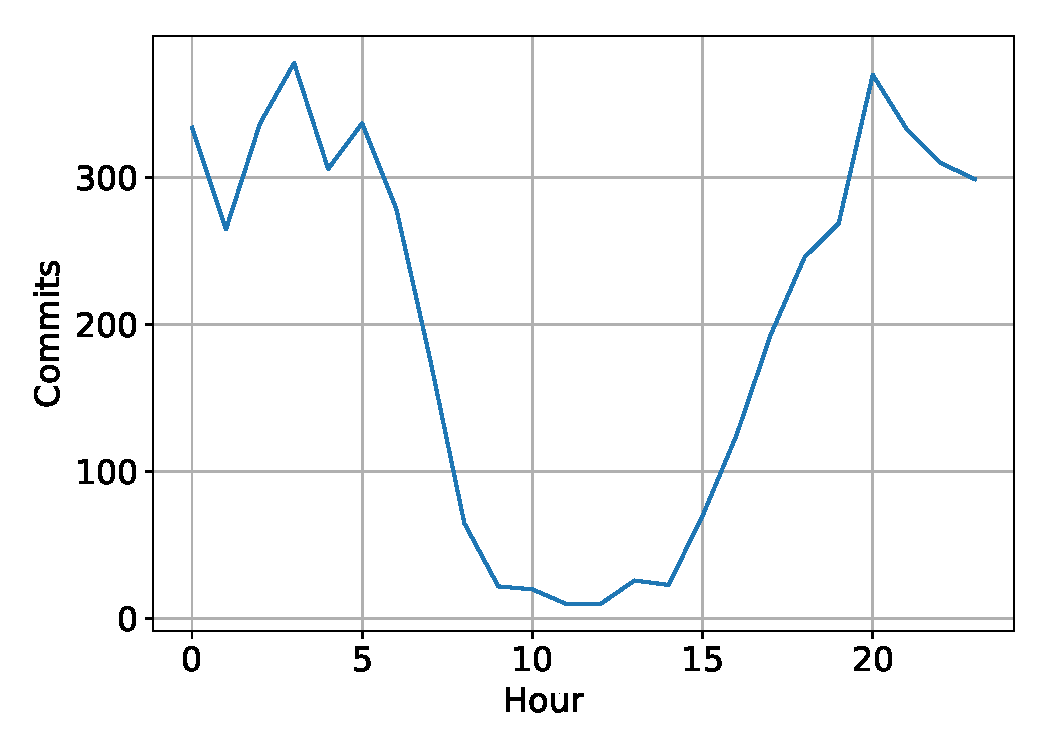
\includegraphics[width=\linewidth]{../figures/obra-intraday.pdf}
    \caption{obra}
    \label{fig:rq1-intraday-obra}
  \end{subfigure}
  %
  \begin{subfigure}{0.3\textwidth}
    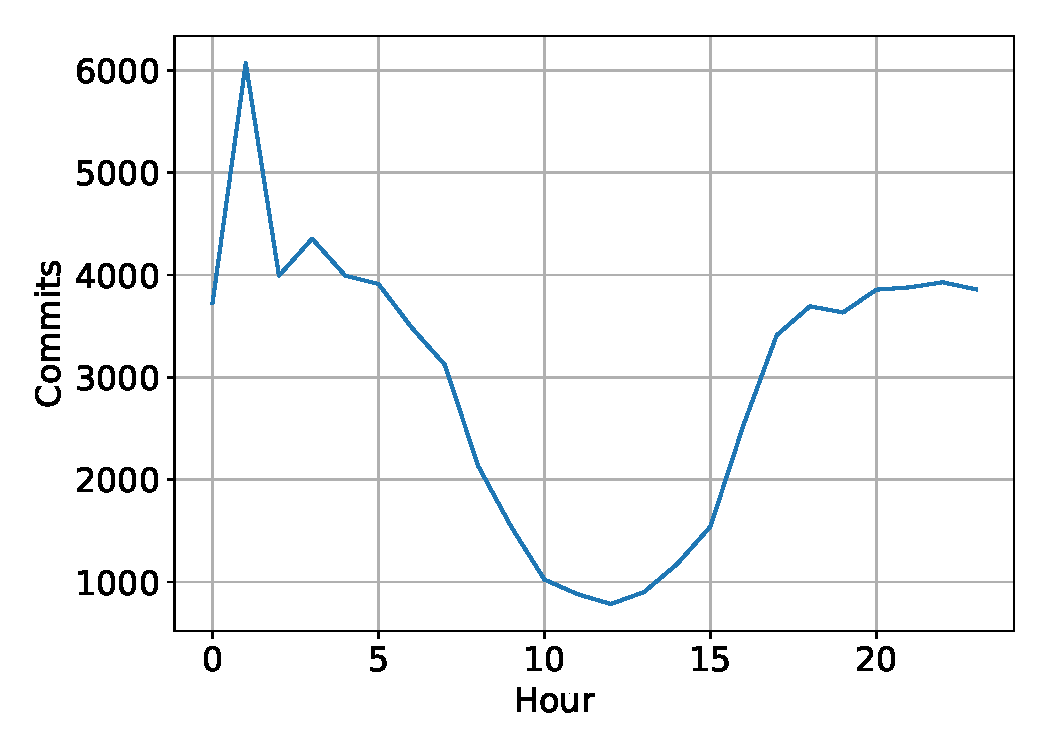
\includegraphics[width=\linewidth]{../figures/Dicklesworthstone-intraday.pdf}
    \caption{Dicklesworthstone}
    \label{fig:rq1-intraday-Dicklesworthstone}
  \end{subfigure}
  %
  \begin{subfigure}{0.3\textwidth}
    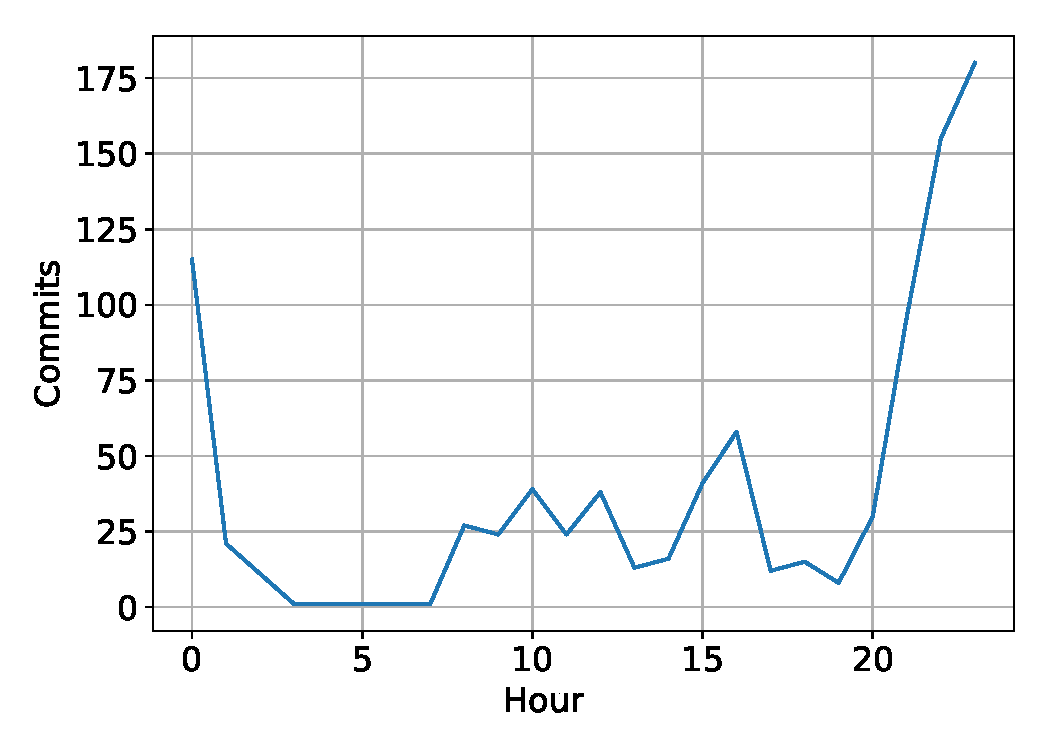
\includegraphics[width=\linewidth]{../figures/philipp-spiess-intraday.pdf}
    \caption{philipp-spiess}
    \label{fig:rq1-intraday-philipp-spiess}
  \end{subfigure}

  \caption{Aggregated commit count per developer per hour (UTC) within a day.}
  \label{fig:rq1-intraday}
\end{figure*}


\textbf{Monthly trajectories are similar but not uniformly sustained.} Three
developers (\texttt{clubanderson}, \texttt{steipete}, and
\texttt{Dicklesworthstone}) sustain increased activity toward the end of the
observation period, whereas the others show high-volume bursts followed by a
decline.


\subsection{RQ2: Coding Agent Harness Usage}
\label{sec:rq2-results}


% harness usage
% - harness signal rate
\subsubsection{Harness signal rate}
The weekly agent harness signal shares for all developers are shown in
\autoref{fig:agent-share-weekly}.

\textbf{Dicklesworthstone and ruvnet have high detected harness-signal rates.}
Dicklesworthstone has a mean of 73\% and a median of 80\% per week (STD =
18.5). Ruvnet has a mean of 75\% and a median of 79\% per week (STD = 20.5).
In both cases, nearly all detected signals identify Claude Code.

\textbf{Philipp-spiess, steipete, and teamchong have low detected
harness-signal rates.} Philipp-spiess has a mean of 5\% and a median of 2\%
(STD = 7.75), steipete has a mean of 3\% and a median of 2\% (STD = 2.5), and
teamchong has a mean of 0.5\%, a median of 0\%, and a maximum of 4.5\% per
week (STD = 1). These low rates may reflect disabled attribution metadata and
harnesses that leave no detectable commit-level trace, rather than an absence of
agent use.

\textbf{The other developers have intermediate detected harness-signal rates.}
Mavam, steveyegge, obra, and clubanderson have agent harness rates between 15\%
and 55\% per week. For clubanderson, the weekly analysis begins in December
2025 because the preceding months contain no substantial activity, as confirmed
in the interview.
We stress that non-attributed commits (those without agent harness signals) may include work by agents that leave no detectable signals (by default or by configuration), as well as genuine manual work.

% - harness frequency (distribution) and diversity
\subsubsection{Harness frequency}
% for each harness, how many commits (and what proportion of total commits) are attributed to it? what does that show?
\textbf{More than half of commits have no detectable harness signal.} Of the
analyzed commits, 7,566 (51.49\%) contain no detectable agent harness signal.
Of the
remaining 71,274 commits, 67,650 (94.92\%) are attributed to Claude Code,
followed by 1,766 with multi-agent signals (2.48\%), 1,087 for Codex (1.53\%),
352 for Copilot (0.49\%), 209 for Amp (0.29\%), and 97 for Gastown (0.14\%).
The remaining harnesses each have less than 0.1\% of the commit share.


\textbf{Harness-signal frequencies reflect both usage and detectability.}
Claude Code's dominance reflects both its adoption and a visibility advantage
from its default attribution settings\footnote{\claudecodeattributionurl}. The
high proportion of non-attributed commits indicates that detection heuristics
may miss AI-assisted work, while the unnormalized distribution is heavily
skewed by a few highly prolific developers.
% what does this mean/show?

\begin{figure}
  \centering
  
\includegraphics[width=.85\linewidth]{figures/rq2/harness-weighted-frequency}
  \caption{Harness frequency weighted by developer. For each harness, the bar shows the mean share of commits attributed to it across developers, normalizing for the differing commit volumes of individual developers.}
  \label{fig:harness-frequency-weighted}
\end{figure}


\subsubsection{Harness diversity}

\textbf{Most developers have a single dominant detectable harness.} Claude Code
is dominant for Dicklesworthstone, obra, clubanderson, mavam, and ruvnet;
OpenAI Codex is dominant for steipete and philipp-spiess.

\textbf{Steveyegge has the most diverse detected harness signals.} Multi-agent
signals from Claude Code and Gastown account for about 20--40\% of commits in
several weeks.

\textbf{No harness signal is the largest category for six developers.} This
applies to clubanderson, mavam, obra, philipp-spiess, steipete, and teamchong.
For steveyegge, Claude Code and no harness signal are nearly tied, at 45.4\%
and 46.1\% of commits, respectively. These results describe detectable traces,
not actual harness diversity: interview evidence indicates that several
developers use additional harnesses or have disabled attribution metadata.

% - harness-switch events
\subsubsection{Harness switch events:} The absolute harness-attributed commit volumes including temporal patterns are shown in \autoref{fig:agent-use-over-time}; the percentage view in \autoref{fig:agent-share-weekly} makes changes in the relative harness composition easier to compare.
Some developers had consistent agent harness signals. Developer Dicklesworthstone only had three weeks with less than 50\% of Claude Code signals, and the agent harness share never changed by more than 25\% week over week. The same applies to ruvnet, except for one week with near-zero commit activity. Similarly, philipp-spiess consistently displayed barely any harness signals, with only three weeks where concrete harness signals accounted for more than 10\% of the commit share, one of them exceeding 30\%. In steipete's case, variability was even lower, and just two weeks exceeded 10\% harness signals. Dicklesworthstone reported using a Claude Code repository-updater skill to aggregate and commit changes, while most code is produced with Codex; its Claude Code signals therefore describe that commit workflow rather than overall harness use.
% To quote them: "I literally do not make anything myself. Like everything is agents. [...] and you can't really rely on the commit messages being accurate in terms of authorship."
Most consistent was developer teamchong, with only 8 weeks containing commits with any agent harness signals, and not a single week exceeding 5\% attribution signal rate.
Other developers showed more fluctuation, both in attribution to non-attribution ratio, and in the concrete agent harnesses the signals were attributed to (clubanderson, mavam, obra, steveyegge).
In general, deviations in agent harness signals were often limited to a single week, and appear to be phases were a developer tried out a different harness, and then went back to their old harness afterwards.
Clear, multi-week changes in agent harness signals can only be observed for clubanderson (no harness signals between the weeks of 2026-02-16 and 2026-04-20, with an exception in the week of 2026-03-23) and mavam (a clear change starting in the week of 2025-12-01, and a more gradual change from 2026-02-09 until 2026-03-16).
Overall we found that agent harness switch events are difficult to gauge. The main source for switch events are changes in the signal to no-harness-signal ratio, which might be more impacted by variations in the workflows leading to commits. More work is needed to identify additional signals and heuristics for identifying harness switch events.

\begin{figure*}[t]
  \centering
  \begin{subfigure}{0.31\textwidth}
    
\includegraphics[width=\linewidth]{figures/rq2/agent-share-weekly-Dicklesworthstone.pdf}
    \caption{Dicklesworthstone}
  \end{subfigure}\hfill
  \begin{subfigure}{0.31\textwidth}
    
\includegraphics[width=\linewidth]{figures/rq2/agent-share-weekly-steipete.pdf}
    \caption{steipete}
  \end{subfigure}\hfill
  \begin{subfigure}{0.31\textwidth}
    
\includegraphics[width=\linewidth]{figures/rq2/agent-share-weekly-teamchong.pdf}
    \caption{teamchong}
  \end{subfigure}

  \begin{subfigure}{0.31\textwidth}
    
\includegraphics[width=\linewidth]{figures/rq2/agent-share-weekly-ruvnet.pdf}
    \caption{ruvnet}
  \end{subfigure}\hfill
  \begin{subfigure}{0.31\textwidth}
    
\includegraphics[width=\linewidth]{figures/rq2/agent-share-weekly-obra.pdf}
    \caption{obra}
  \end{subfigure}\hfill
  \begin{subfigure}{0.31\textwidth}
    
\includegraphics[width=\linewidth]{figures/rq2/agent-share-weekly-mavam.pdf}
    \caption{mavam}
  \end{subfigure}

  \begin{subfigure}{0.31\textwidth}
    
\includegraphics[width=\linewidth]{figures/rq2/agent-share-weekly-philipp-spiess.pdf}
    \caption{philipp-spiess}
  \end{subfigure}\hfill
  \begin{subfigure}{0.31\textwidth}
    
\includegraphics[width=\linewidth]{figures/rq2/agent-share-weekly-steveyegge.pdf}
    \caption{steveyegge}
  \end{subfigure}\hfill
  \begin{subfigure}{0.31\textwidth}
    
\includegraphics[width=\linewidth]{figures/rq2/agent-share-weekly-clubanderson.pdf}
    \caption{clubanderson}
  \end{subfigure}
  \caption{Weekly share of commits attributed to each detected agent harness for every developer. The line indicates weekly commit volume.}
  \label{fig:agent-share-weekly}
\end{figure*}

\begin{figure*}[t]
  \centering
  \begin{subfigure}{0.31\textwidth}
    
\includegraphics[width=\linewidth]{figures/rq2/rq2-agent-use-Dicklesworthstone.pdf}
    \caption{Dicklesworthstone}
  \end{subfigure}\hfill
  \begin{subfigure}{0.31\textwidth}
    
\includegraphics[width=\linewidth]{figures/rq2/rq2-agent-use-steipete.pdf}
    \caption{steipete}
  \end{subfigure}\hfill
  \begin{subfigure}{0.31\textwidth}
    
\includegraphics[width=\linewidth]{figures/rq2/rq2-agent-use-teamchong.pdf}
    \caption{teamchong}
  \end{subfigure}

  \begin{subfigure}{0.31\textwidth}
    
\includegraphics[width=\linewidth]{figures/rq2/rq2-agent-use-ruvnet.pdf}
    \caption{ruvnet}
  \end{subfigure}\hfill
  \begin{subfigure}{0.31\textwidth}
    
\includegraphics[width=\linewidth]{figures/rq2/rq2-agent-use-obra.pdf}
    \caption{obra}
  \end{subfigure}\hfill
  \begin{subfigure}{0.31\textwidth}
    
\includegraphics[width=\linewidth]{figures/rq2/rq2-agent-use-mavam.pdf}
    \caption{mavam}
  \end{subfigure}

  \begin{subfigure}{0.31\textwidth}
    
\includegraphics[width=\linewidth]{figures/rq2/rq2-agent-use-philipp-spiess.pdf}
    \caption{philipp-spiess}
  \end{subfigure}\hfill
  \begin{subfigure}{0.31\textwidth}
    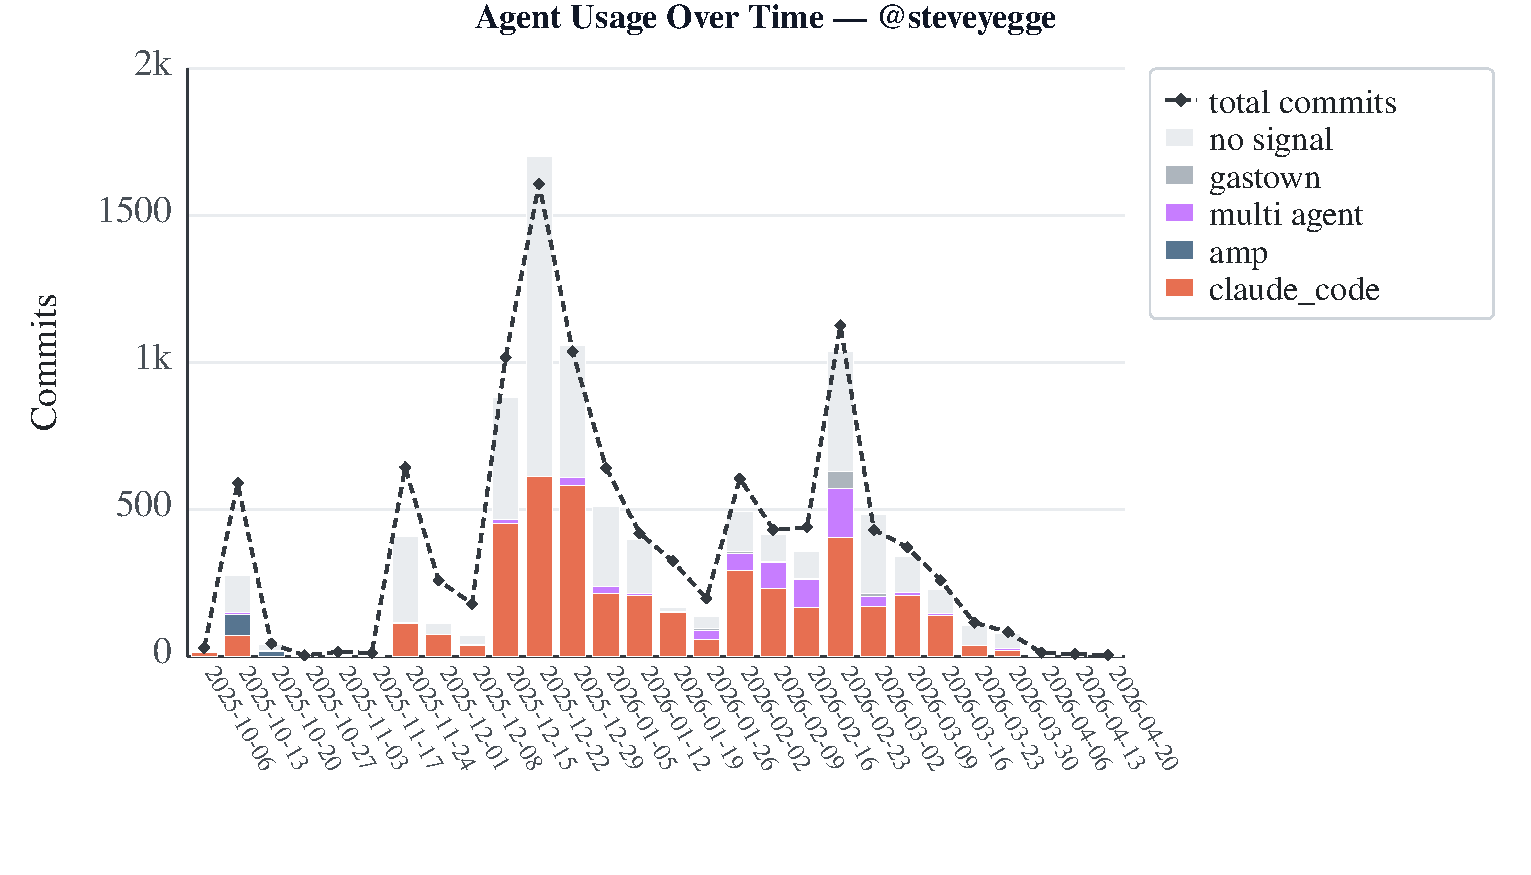
\includegraphics[width=\linewidth]{figures/rq2/rq2-agent-use-steveyegge.pdf}
    \caption{steveyegge}
  \end{subfigure}\hfill
  \begin{subfigure}{0.31\textwidth}
    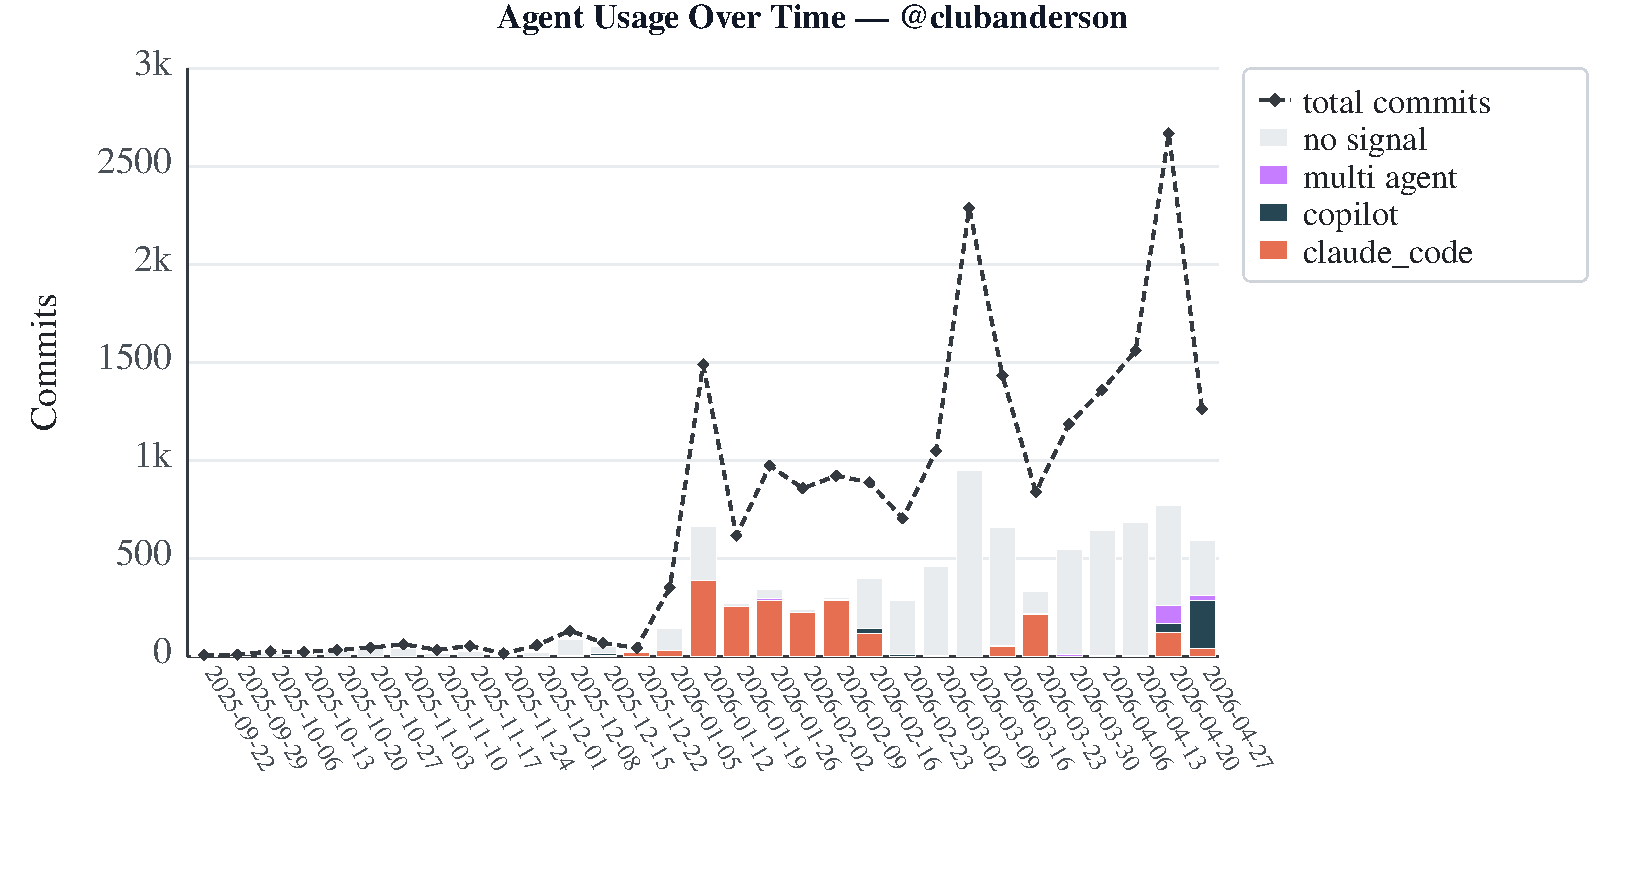
\includegraphics[width=\linewidth]{figures/rq2/rq2-agent-use-clubanderson.pdf}
    \caption{clubanderson}
  \end{subfigure}
  \caption{Absolute weekly commit volumes attributed to each detected agent harness for every developer. The line indicates total weekly commits; harnesses with fewer than 50 commits over the observation period are omitted from the stacked bars.}
  \label{fig:agent-use-over-time}
\end{figure*}

\subsubsection{Task-Harness Coupling}

\textbf{Task--harness patterns are dominated by Claude Code and unattributed
commits.} \texttt{chore} and \texttt{feat} are mostly associated with Claude
Code, whereas \texttt{build}, \texttt{ci}, \texttt{docs}, \texttt{perf},
\texttt{refactor}, and \texttt{revert} are predominantly unattributed
(\autoref{fig:agents-by-commit-type-percentage}).

\textbf{Conventional Commit label coverage varies sharply by harness.} The share
of commits without a recognized Conventional Commit type is 90\% for GitHub
Copilot but only 10\% for Claude Code, and lower for several other harnesses.
This may reflect either default harness behavior or developer-authored commit
messages.

\textbf{Five task labels account for the most common labeled work.} Across
harnesses, unattributed commits, and the full corpus, the three most common
labeled tasks always fall within \texttt{feat}, \texttt{fix}, \texttt{docs},
\texttt{chore}, and \texttt{refactor}. \texttt{revert}, \texttt{style},
\texttt{perf}, and \texttt{ci} occur too rarely to characterize most harnesses
reliably.

\textbf{Several harnesses have narrow detected task profiles.} While
\texttt{feat} and \texttt{fix} appear across all harnesses, Qwen Code is limited
to \texttt{feat}, \texttt{fix}, \texttt{docs}, and \texttt{chore}; Cursor shows
a similarly narrow profile but includes \texttt{test}. Codex has
\texttt{docs} as its largest category while covering more task types, whereas
Copilot is concentrated in \texttt{feat}, \texttt{fix}, and \texttt{chore}.
Qwen Code exclusively uses Conventional Commit labels. Interview evidence
corroborates task-specific harness selection, including Gemini for code review
and Claude Code for orchestration.

% We provide a fine-grained analysis that reports agent-task distribution for each developer independently in \autoref{agent-harness-per-task-per-dev}. We note that 46\% of labeled commits are attributed to Claude Code and 51.5\% have no harness signal, so aggregate task-harness comparisons are likely to display this imbalance to some extent. But wether the observed task-harness couplings reflect deliberate tool choice (e.g., using Codex when writing documentation), statistical artifacts of the usage distribution, or related to harness default behavior (e.g., no attribution signals for harnesses that are frequently used for docs), remains an open question for future work.

% - distribution of commit categories (task types) per harness
% - differences in harness usage across development tasks

\begin{figure*}[t]
  \centering
  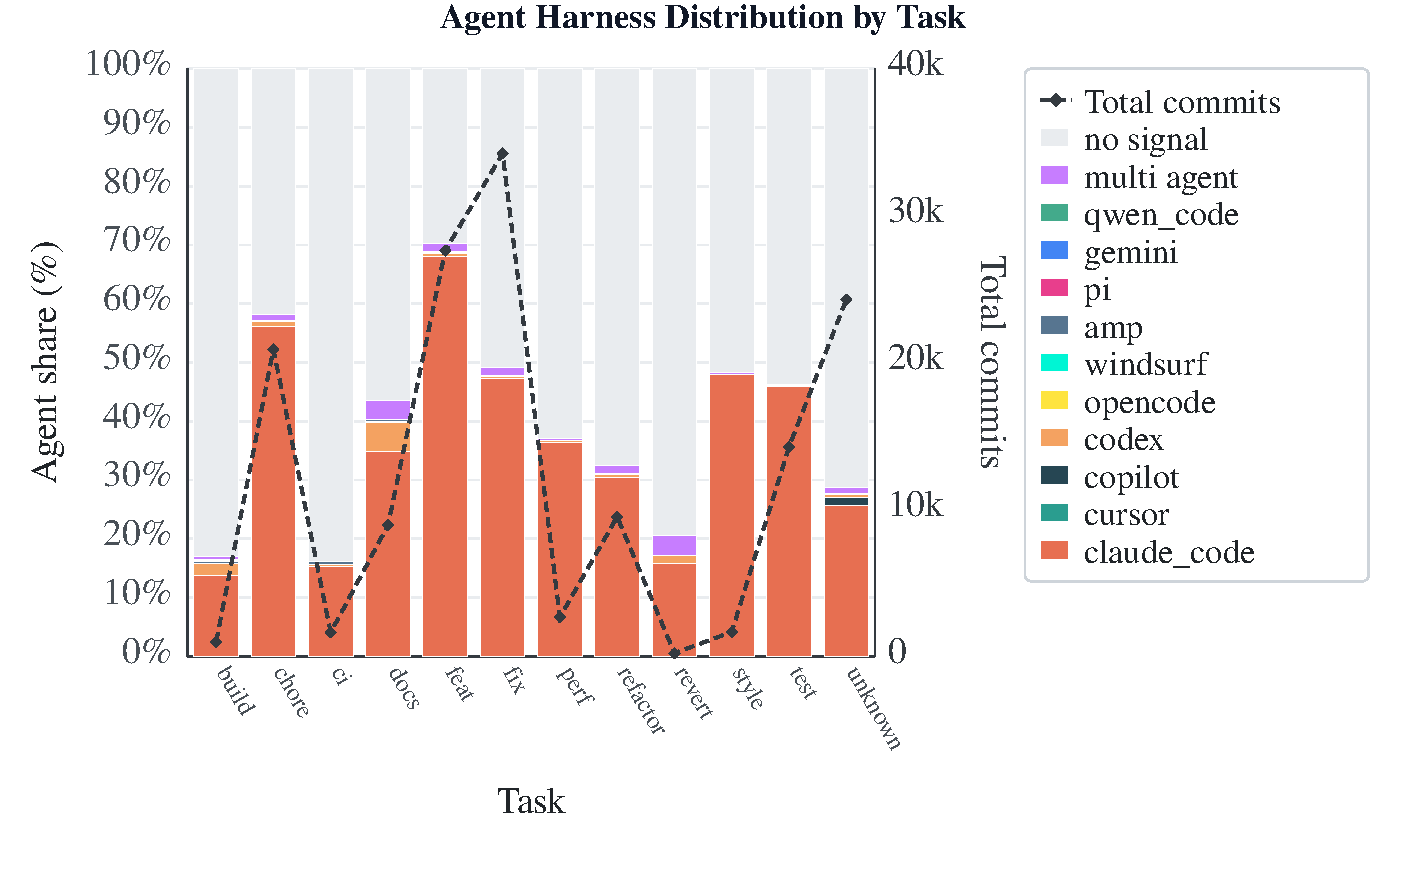
\includegraphics[width=0.8\linewidth]{figures/rq2/agents-by-commit-type-percentage.pdf}
  \caption{Agent harness distribution by task type. Each stacked column shows the percentage of commits for a task attributed to each agent harness; the line indicates the total number of commits for that task.}
  \label{fig:agents-by-commit-type-percentage}
\end{figure*}

\begin{figure*}[t]
  \centering
  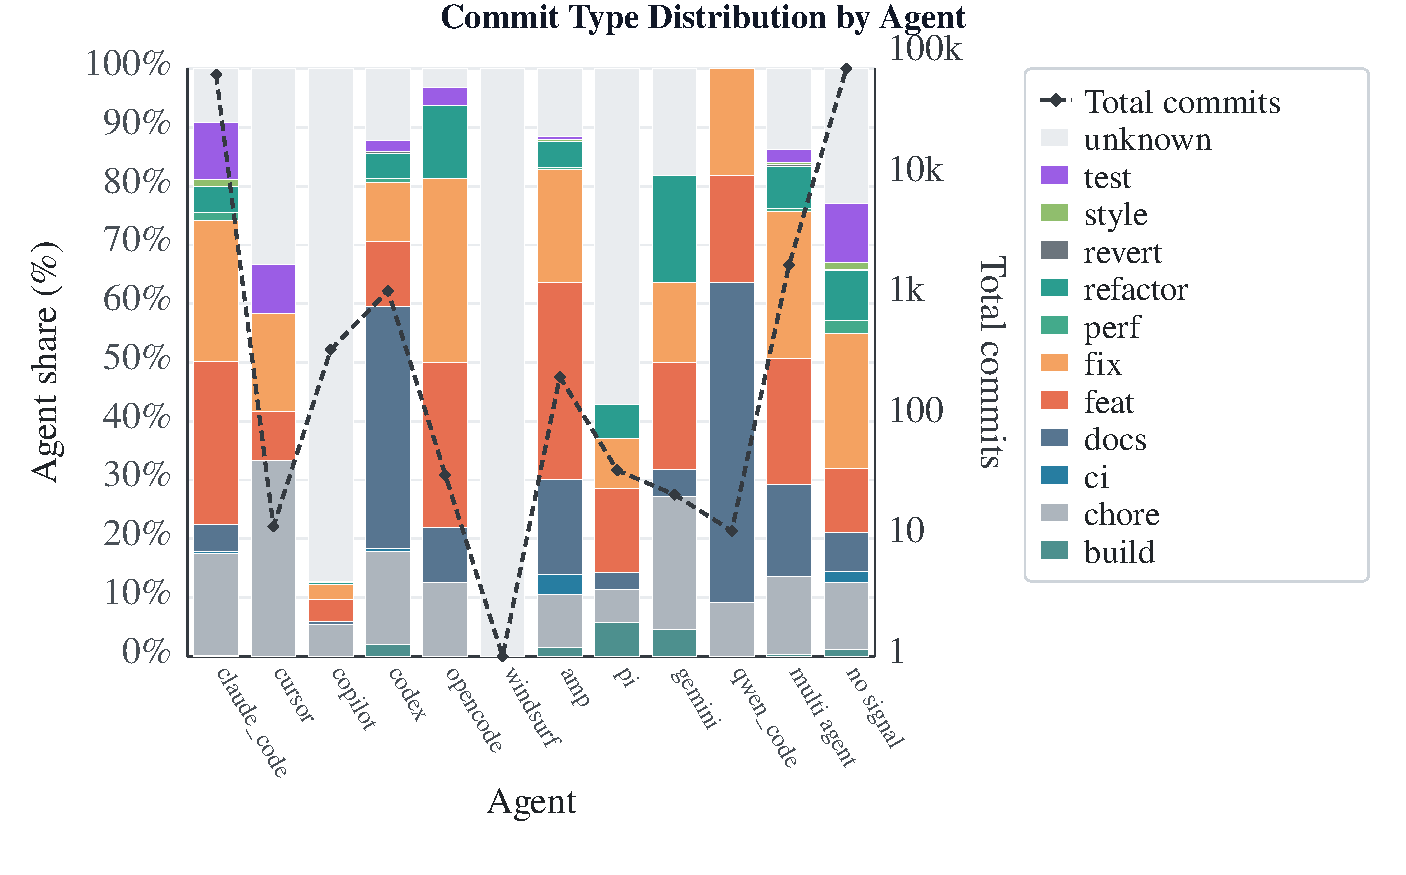
\includegraphics[width=0.8\linewidth]{figures/rq2/commit-types-by-agent-percentage-log.pdf}
  \caption{Distribution of commit types by agent harness, showing the percentage of each task type performed by different agents.}
  \label{fig:commit-types-by-agent-percentage-log}
\end{figure*}

\begin{figure*}[t]
  \centering
  \begin{subfigure}{0.3\textwidth}
    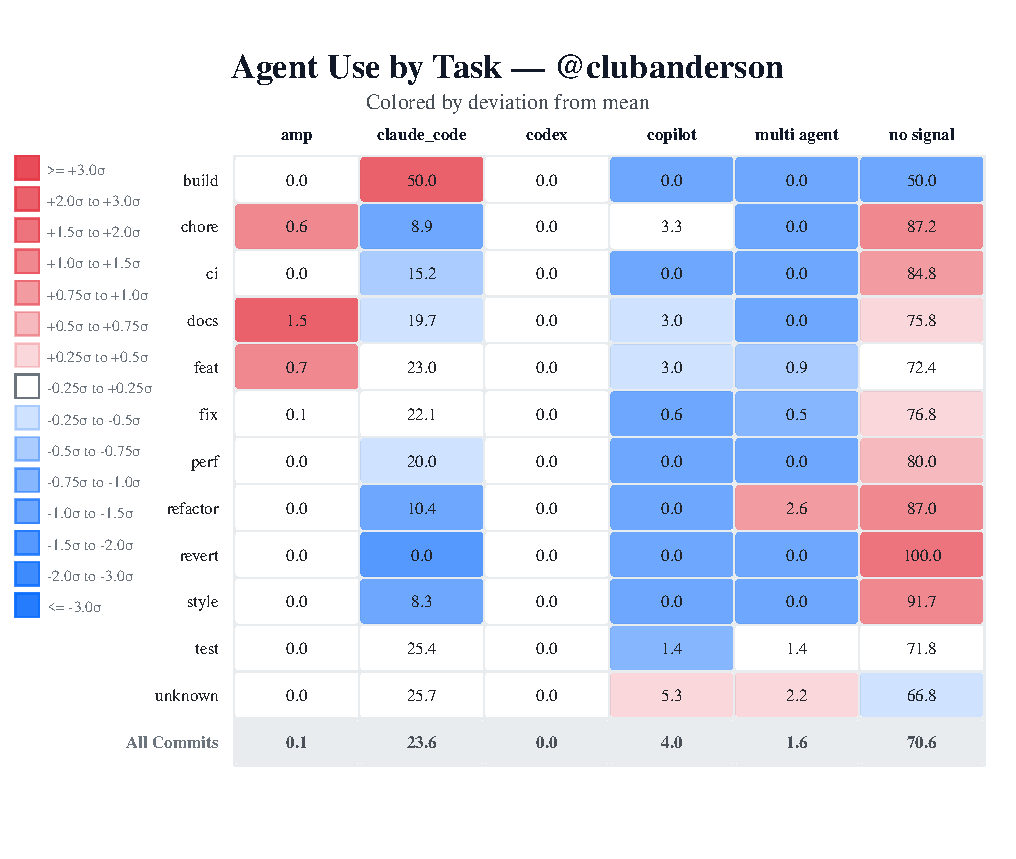
\includegraphics[width=\linewidth]{figures/rq2/clubanderson-colored-table.pdf}
    \caption{clubanderson}
    \label{fig:clubanderson-colored-table}
  \end{subfigure}
  \hfill
  \begin{subfigure}{0.3\textwidth}
    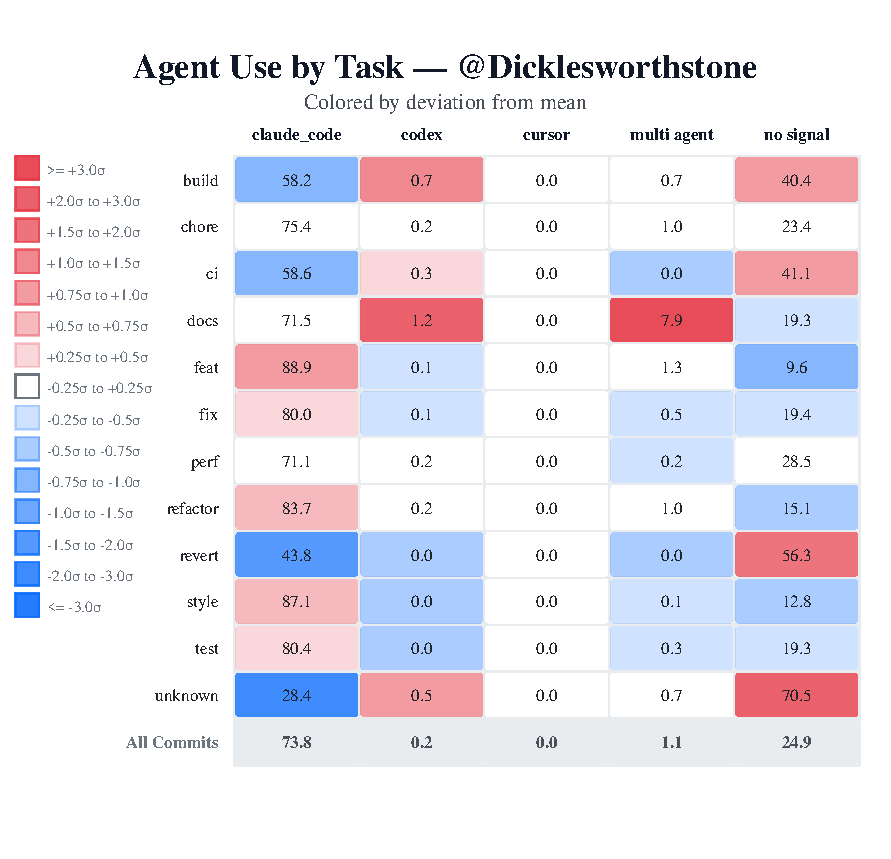
\includegraphics[width=\linewidth]{figures/rq2/Dicklesworthstone-colored-table.pdf}
    \caption{Dicklesworthstone}
    \label{fig:Dicklesworthstone-colored-table}
  \end{subfigure}
  \hfill
  \begin{subfigure}{0.3\textwidth}
    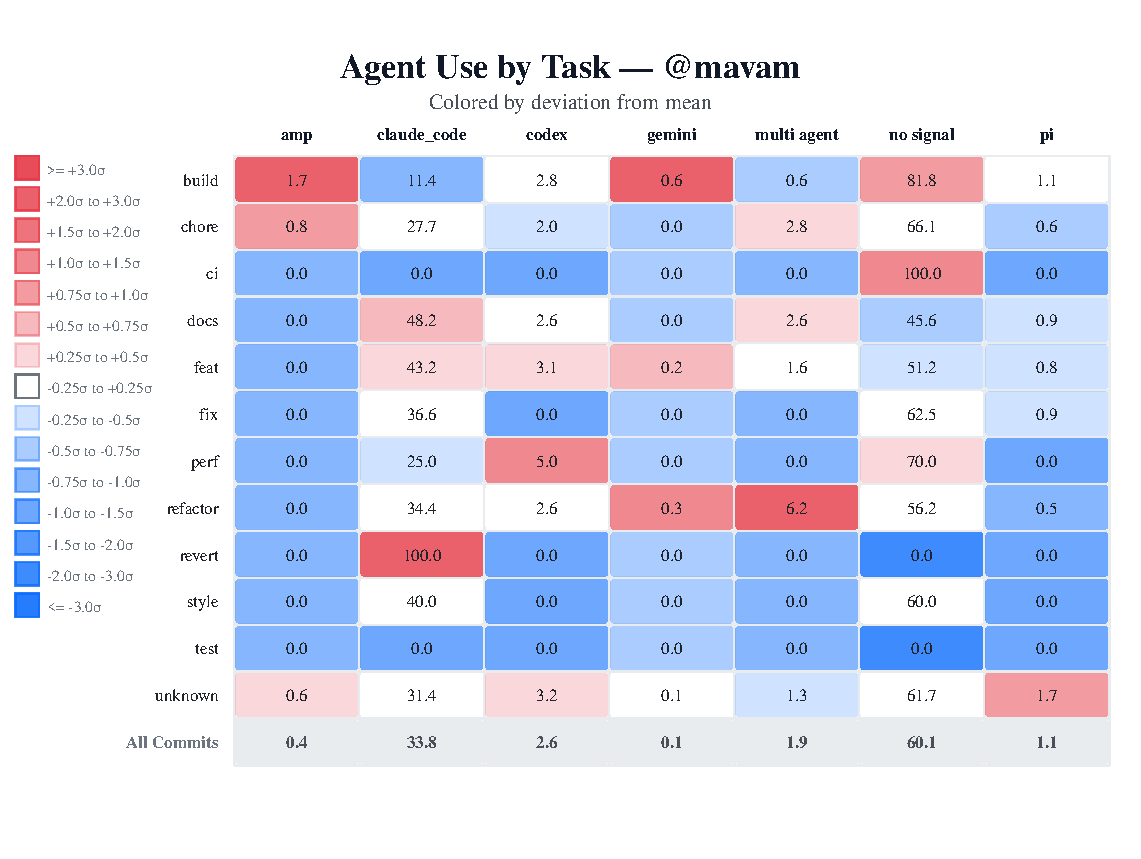
\includegraphics[width=\linewidth]{figures/rq2/mavam-colored-table.pdf}
    \caption{mavam}
    \label{fig:mavam-colored-table}
  \end{subfigure}
  \vspace{0.5em}
  \begin{subfigure}{0.3\textwidth}
    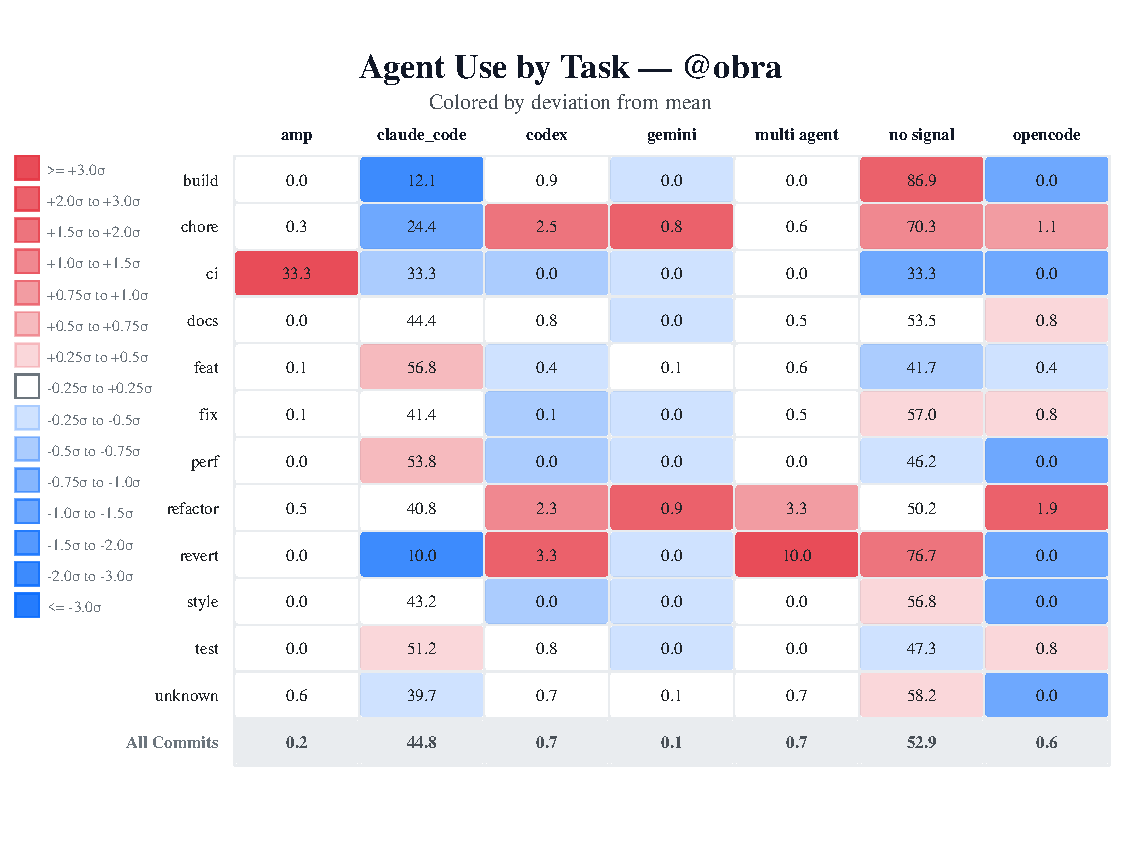
\includegraphics[width=\linewidth]{figures/rq2/obra-colored-table.pdf}
    \caption{obra}
    \label{fig:obra-colored-table}
  \end{subfigure}
  \hfill
  \begin{subfigure}{0.3\textwidth}
    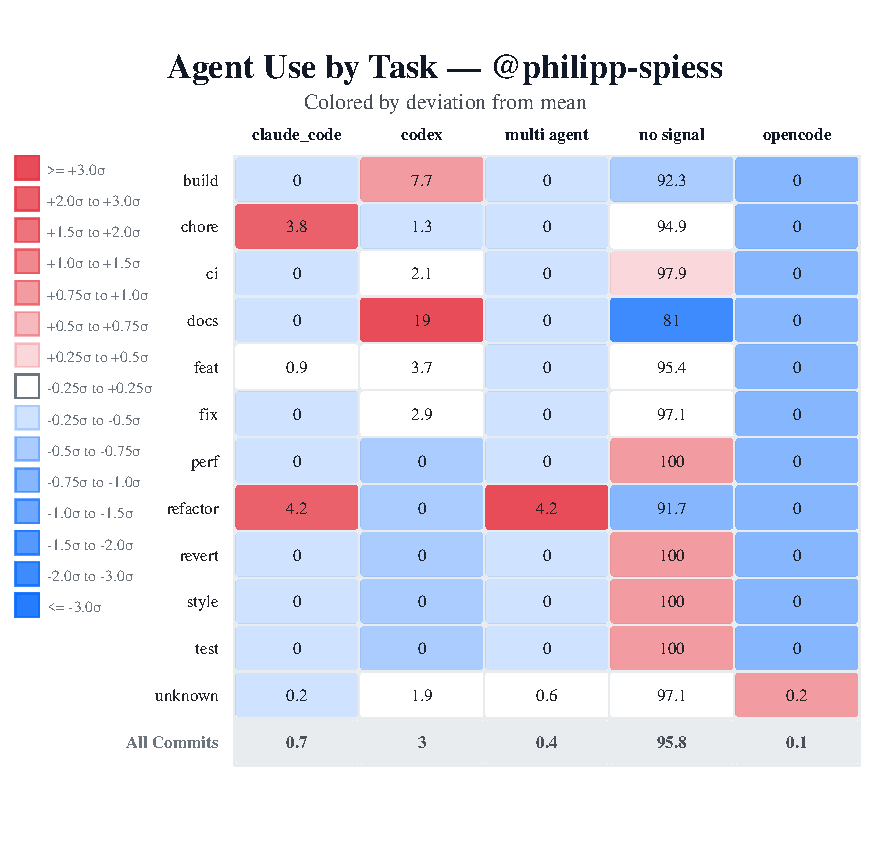
\includegraphics[width=\linewidth]{figures/rq2/philipp-spiess-colored-table.pdf}
    \caption{philipp-spiess}
    \label{fig:philipp-spiess-colored-table}
  \end{subfigure}
  \hfill
  \begin{subfigure}{0.3\textwidth}
    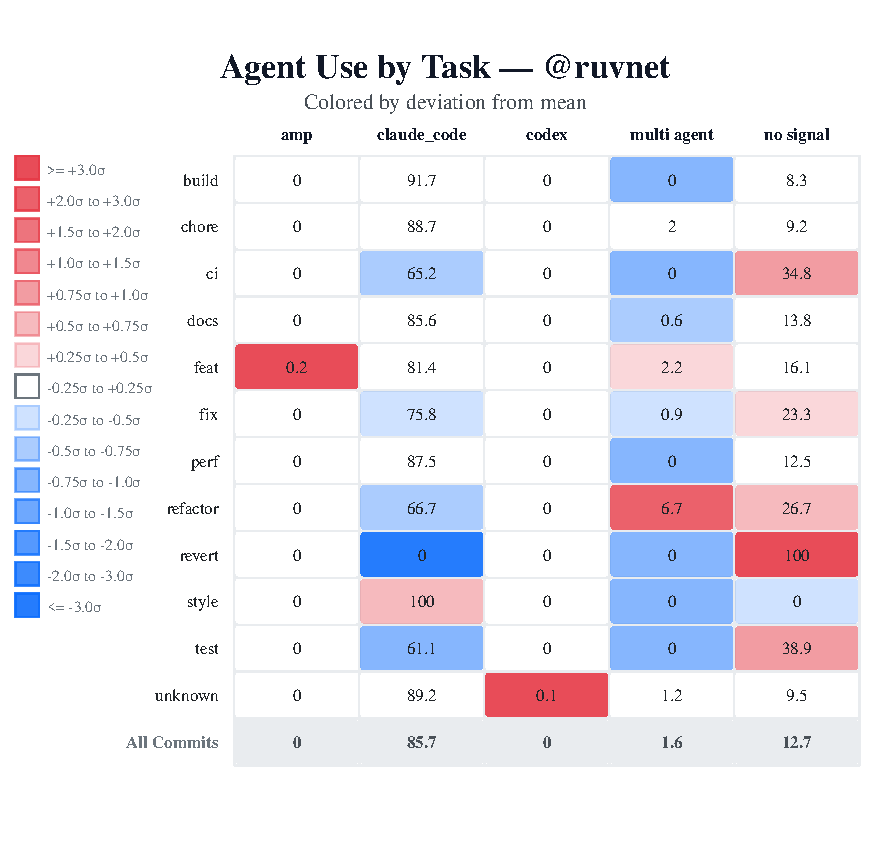
\includegraphics[width=\linewidth]{figures/rq2/ruvnet-colored-table.pdf}
    \caption{ruvnet}
    \label{fig:ruvnet-colored-table}
  \end{subfigure}
  \vspace{0.5em}
  \begin{subfigure}{0.3\textwidth}
    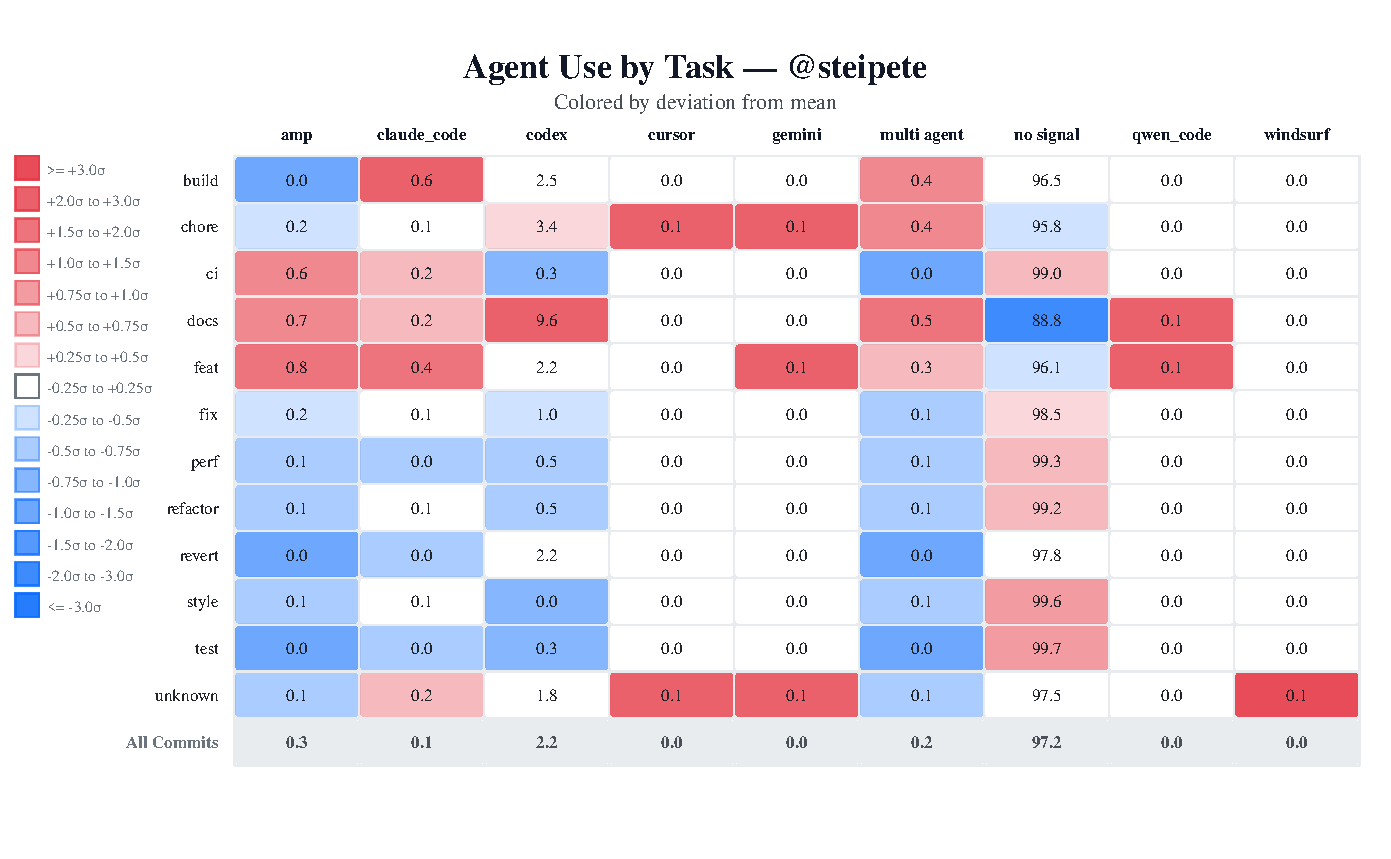
\includegraphics[width=\linewidth]{figures/rq2/steipete-colored-table.pdf}
    \caption{steipete}
    \label{fig:steipete-colored-table}
  \end{subfigure}
  \hfill
  \begin{subfigure}{0.3\textwidth}
    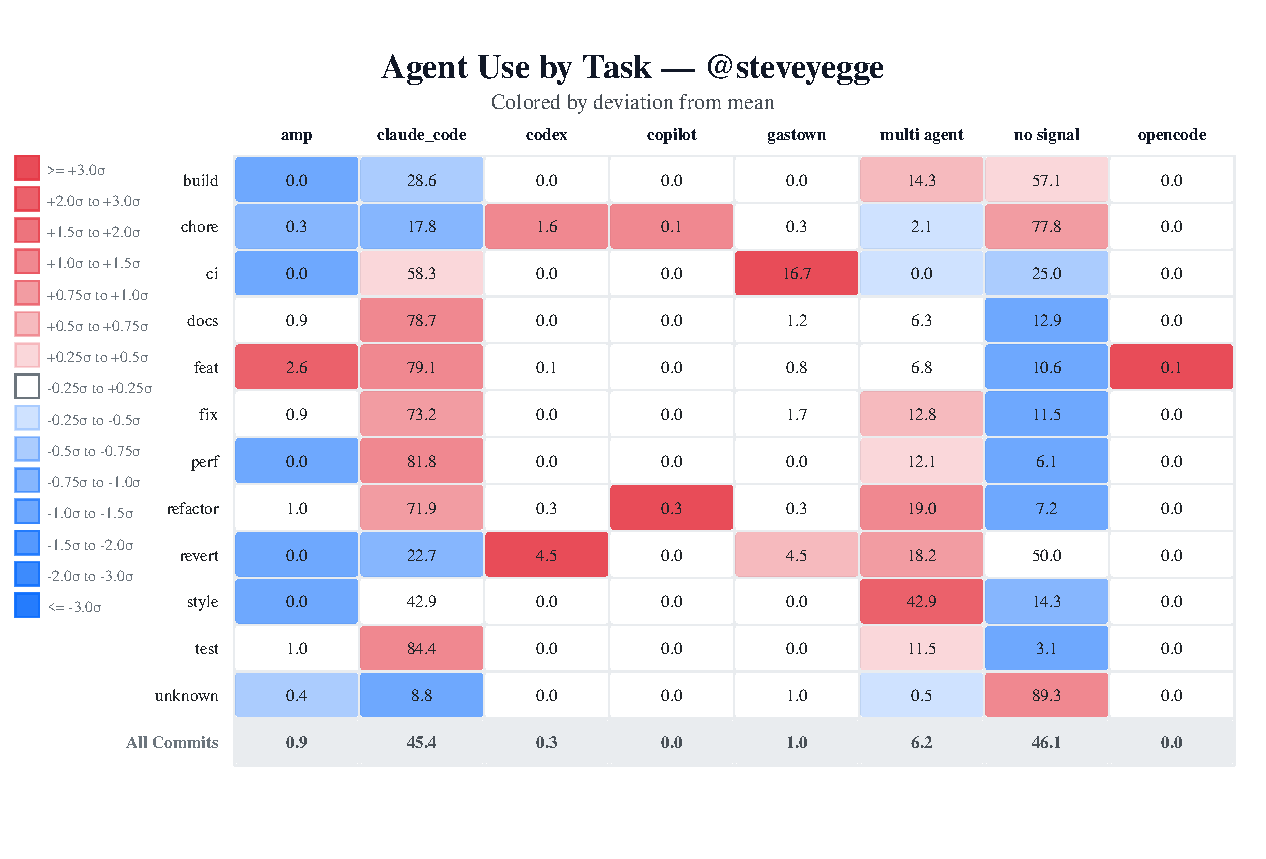
\includegraphics[width=\linewidth]{figures/rq2/steveyegge-colored-table.pdf}
    \caption{steveyegge}
    \label{fig:steveyegge-colored-table}
  \end{subfigure}
  \hfill
  \begin{subfigure}{0.3\textwidth}
    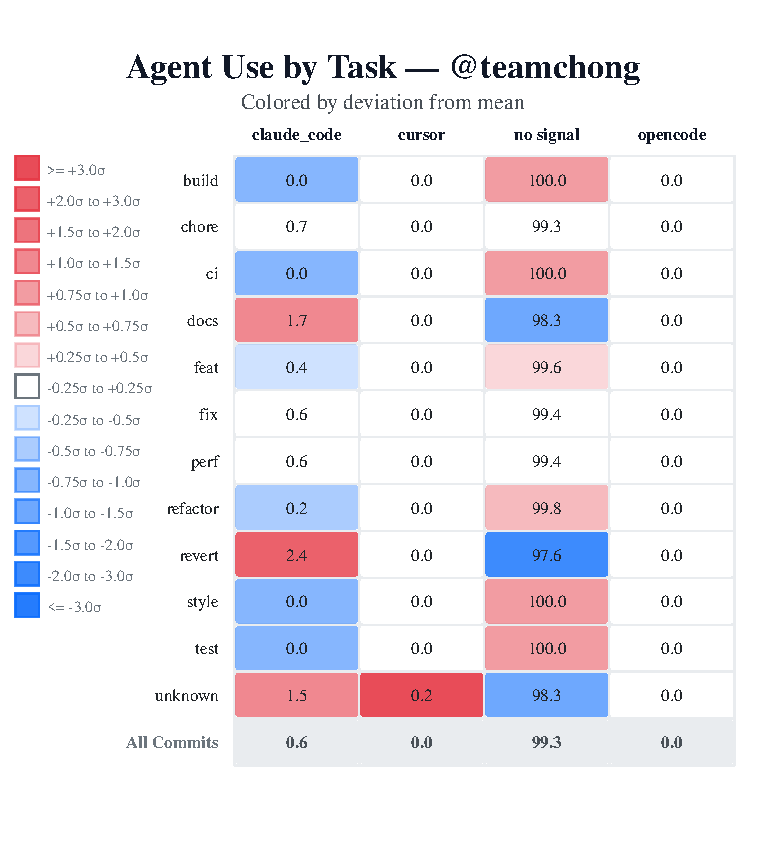
\includegraphics[width=\linewidth]{figures/rq2/teamchong-colored-table.pdf}
    \caption{teamchong}
    \label{fig:teamchong-colored-table}
  \end{subfigure}
  \caption{Colored tables for task-harness coupling for each developer, showing deviations from the baseline distribution. Color intensity indicates the magnitude of deviation.}
  \label{fig:colored-tables}
\end{figure*}


% conclusion, classification
% - substantial differences in commit behavior between different harnesses
% - conventional commits can serve as a signal, but aren't always available
% - our analysis suggests certain agent harnesses might be used for specific tasks
% - overall, Claude Code leaves the most traces, followed by OpenAI Codex, while other harnesses rarely leave any traces 
\textbf{Conventional Commit labels are a complementary, incomplete harness
signal.} Harnesses differ in their Conventional Commit label coverage and task
distribution, but the labels are not present in every commit and cannot identify
harnesses in isolation.

\textbf{Claude Code leaves the most detectable traces.} Codex is second, while
other harnesses rarely leave traces. Their usage may therefore be substantially
undercounted, limiting statistical evaluation.


\subsection{RQ3: Repository Switching Behavior}

Figure~\ref{fig:rq4-four-devs} illustrates the repository-switching behavior of four representative developers: Dicklesworthstone and steipete as examples of high-switching developers, and teamchong and steveyegge as examples of more average-switching developers.

\textbf{Repository breadth varies substantially across developers.} Across all
developer-weeks, developers maintained activity in a mean of 7.20 repositories.
Dicklesworthstone and steipete maintained activity across a large number of
repositories (means of 28.15 and 11.28 active repositories per week,
respectively), whereas teamchong and steveyegge typically worked on a smaller
set of repositories (means of 2.45 and 1.78).
%   - Per-developer (min, max, mean, median active repos/week):
%     - Dicklesworthstone — 0, 93, 28.15, 26.5
%     - steipete          — 1, 55, 11.28, 7.5
%     - teamchong         — 0, 8, 2.45, 2.0
%     - mavam             — 1, 15, 5.70, 5.0
%     - steveyegge        — 0, 3, 1.78, 2.0
%     - obra              — 0, 11, 4.24, 4.0

\textbf{Repository activity is moderately concentrated overall.} The median
weekly Gini coefficient is 0.449. Developers with the largest number of active
repositories also have the highest concentration (Dicklesworthstone: 0.686;
steipete: 0.748), indicating that most activity remains focused on a few
dominant projects. Developers with fewer active repositories generally have
lower concentration (teamchong: 0.350; steveyegge: 0.092).
% - Selected per-developer median Gini: Dicklesworthstone 0.686; steipete 0.748; teamchong 0.350; mavam 0.483; steveyegge 0.092; obra 0.488.

\textbf{Most developers work in one repository per session but switch several
times a day.} The median number of daily repository switches is 4.0.
Dicklesworthstone and steipete have exceptionally high daily switching
rates. Dicklesworthstone has a median of 168.5 and a maximum of 1,292
switches per day; steipete has a median of 18.0 and a maximum of 355 switches
per day.
% - Day-level maxima: Dicklesworthstone = 1292, steipete = 355, clubanderson = 194, teamchong = 154.
% - Day-level medians: Dicklesworthstone = 168.5, steipete = 18.0, teamchong = 2.0.
% - Session-level medians: Dicklesworthstone = 4.0; most other developers = 0.0.

\textbf{The cohort has broader repository engagement than the pre-AI baseline.}
Vasilescu et al.~\cite{Vasilescu2016sky} report a mean of 3.7 repositories per
week (median: 3; maximum: 18), whereas this cohort averages 7.2 active
repositories per week with a median of 5.0 and a maximum of 93. Both the mean
and median exceed the baseline.

% - Notable patterns: a small number of developers (Dicklesworthstone, steipete) drive high breadth and extreme daily switch maxima; most developers show low median daily and session switches.

% - Caveat: some high-volume days were sampled (see `sampled\_commits` vs `reported\_commits` in `data/exports-RQ4`), so absolute maxima may be affected by collection choices.

\begin{figure*}[t]
  \centering
  \begin{subfigure}{\textwidth}
    \centering
    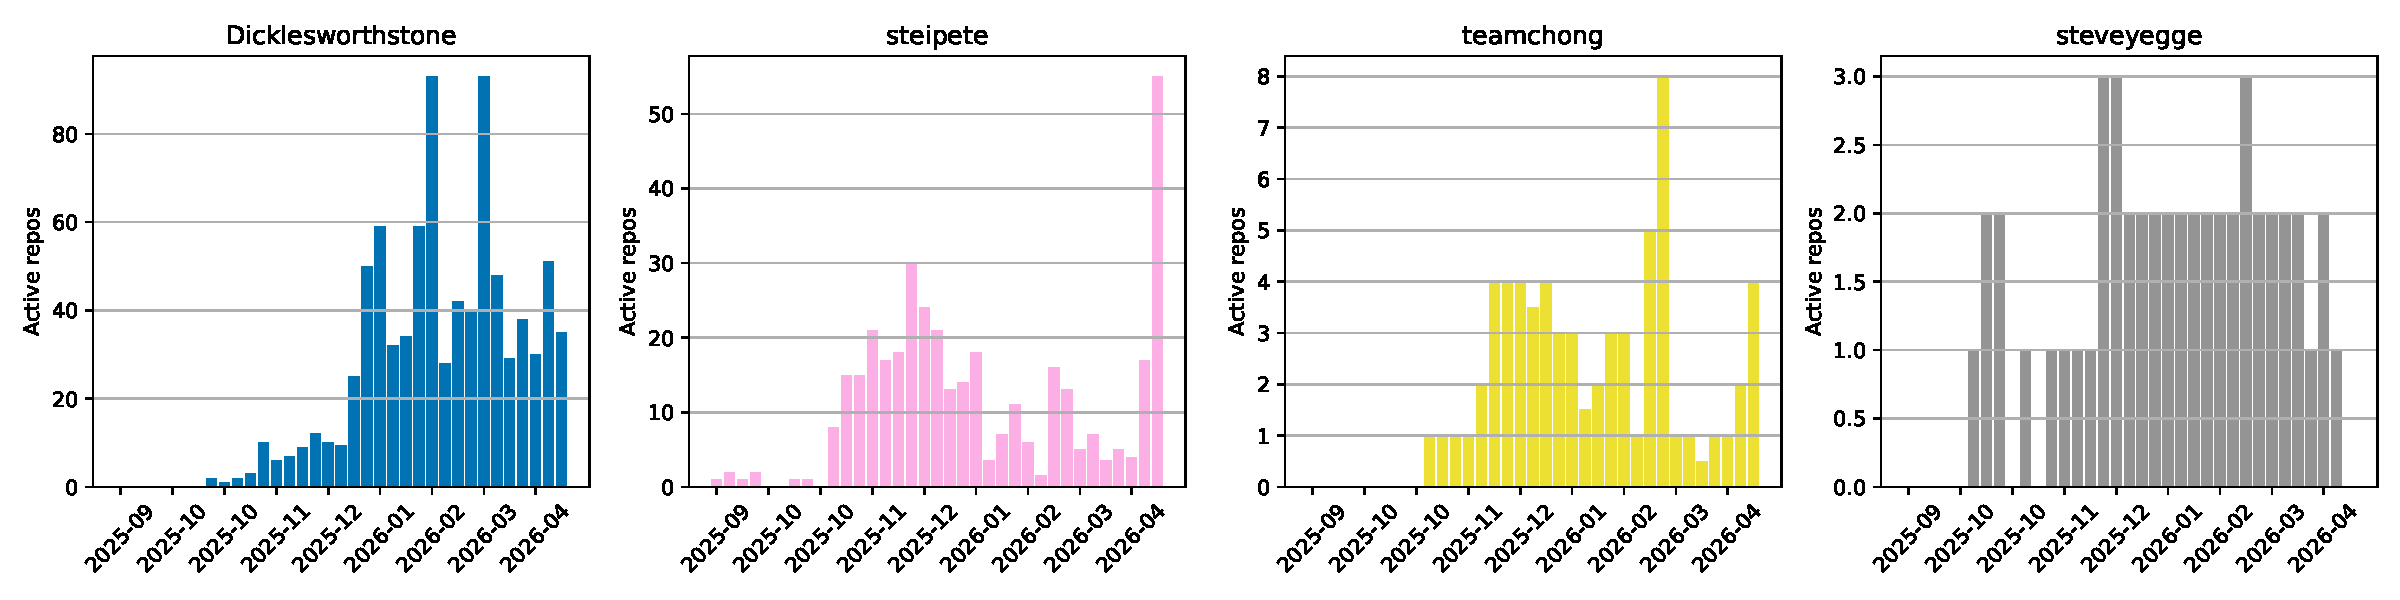
\includegraphics[width=\linewidth]{../data/exports-RQ4/plots/active_repos_four_devs_row.pdf}
    \caption{Active repositories per week.}
    \label{fig:rq4-active-four}
  \end{subfigure}
  \begin{subfigure}{\textwidth}
  \vspace{0.5em}
    \centering
    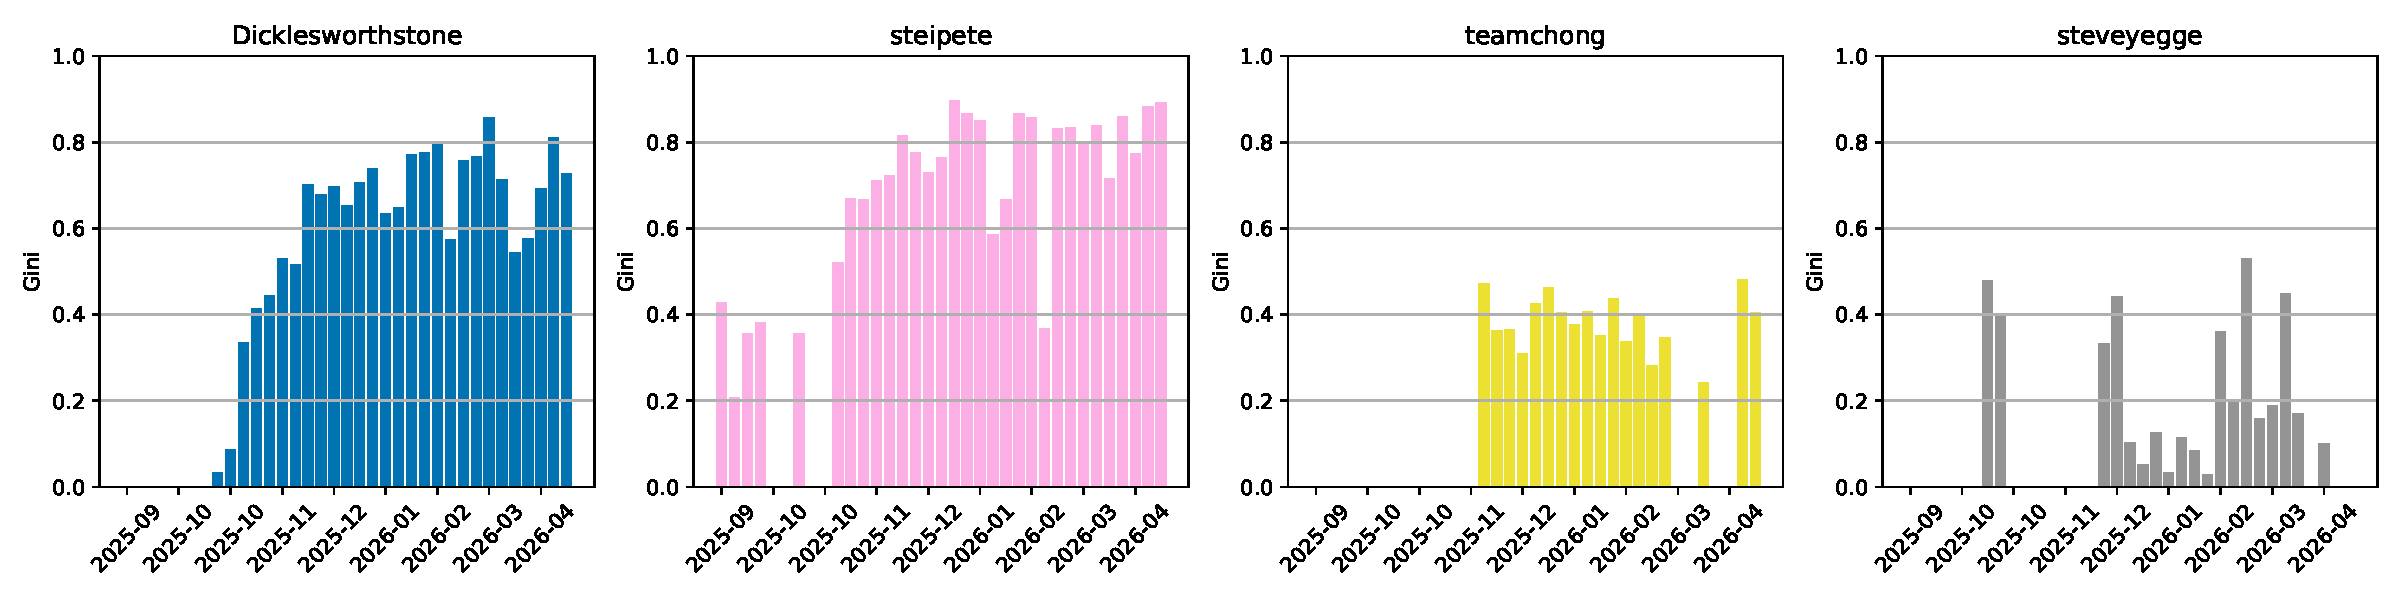
\includegraphics[width=\linewidth]{../data/exports-RQ4/plots/gini_four_devs_row.pdf}
    \caption{Gini coefficient per week.}
    \label{fig:rq4-gini-four}
  \end{subfigure}
  \vspace{0.5em}
  \begin{subfigure}{\textwidth}
    \centering
    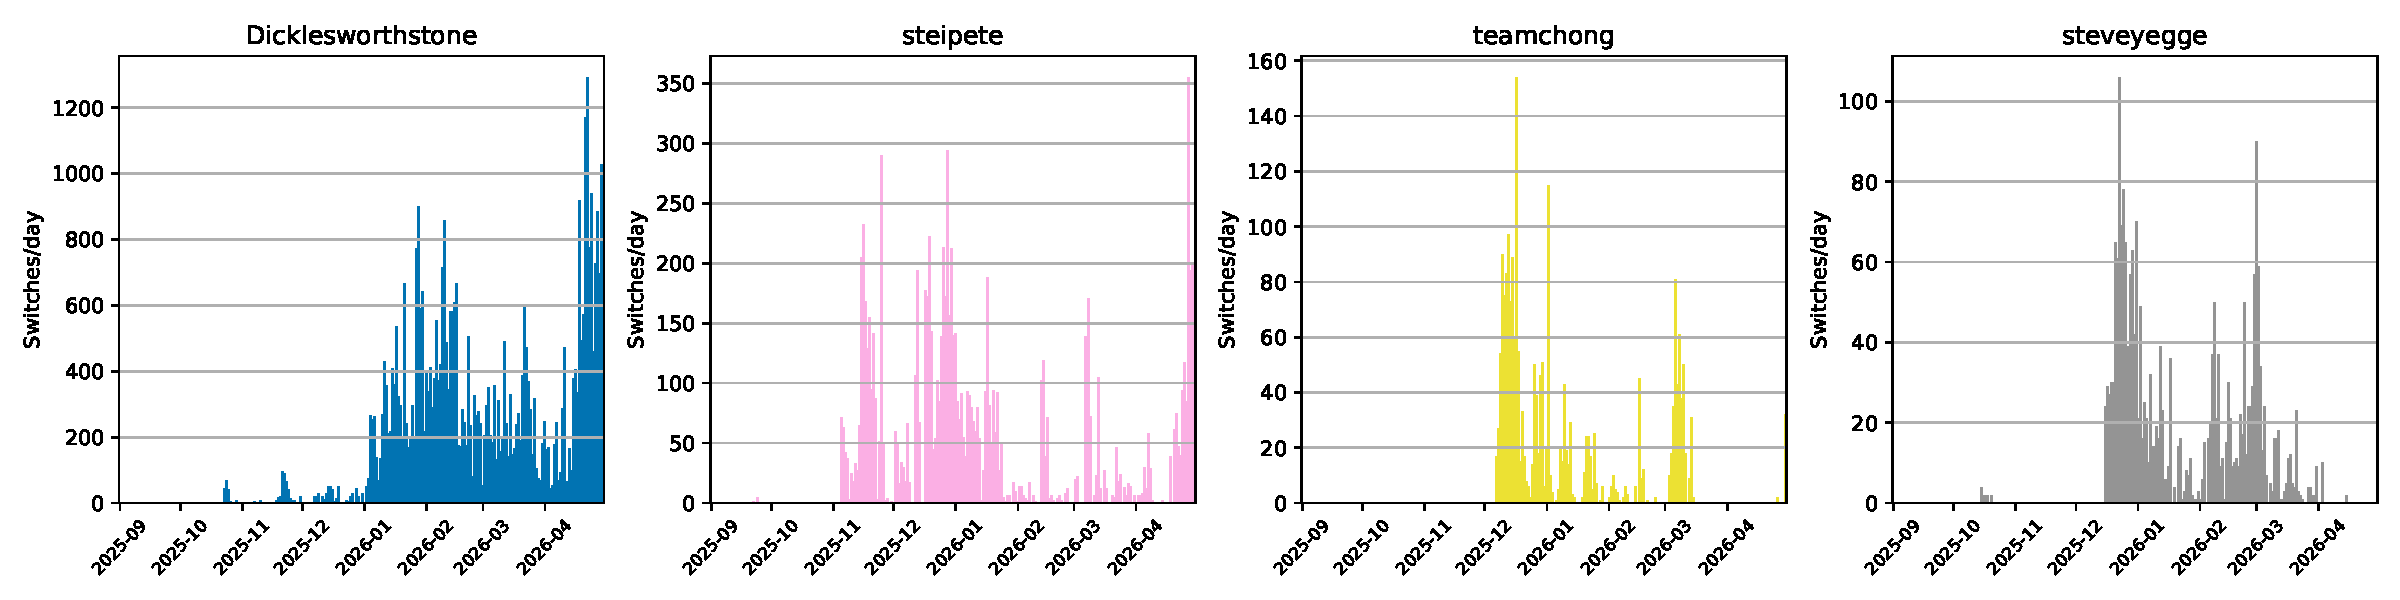
\includegraphics[width=\linewidth]{../data/exports-RQ4/plots/switches_day_four_devs_row.pdf}
    \caption{Repository switches per day.}
    \label{fig:rq4-switches-day-four}
  \end{subfigure}
  \vspace{0.5em}
  \begin{subfigure}{\textwidth}
    \centering
    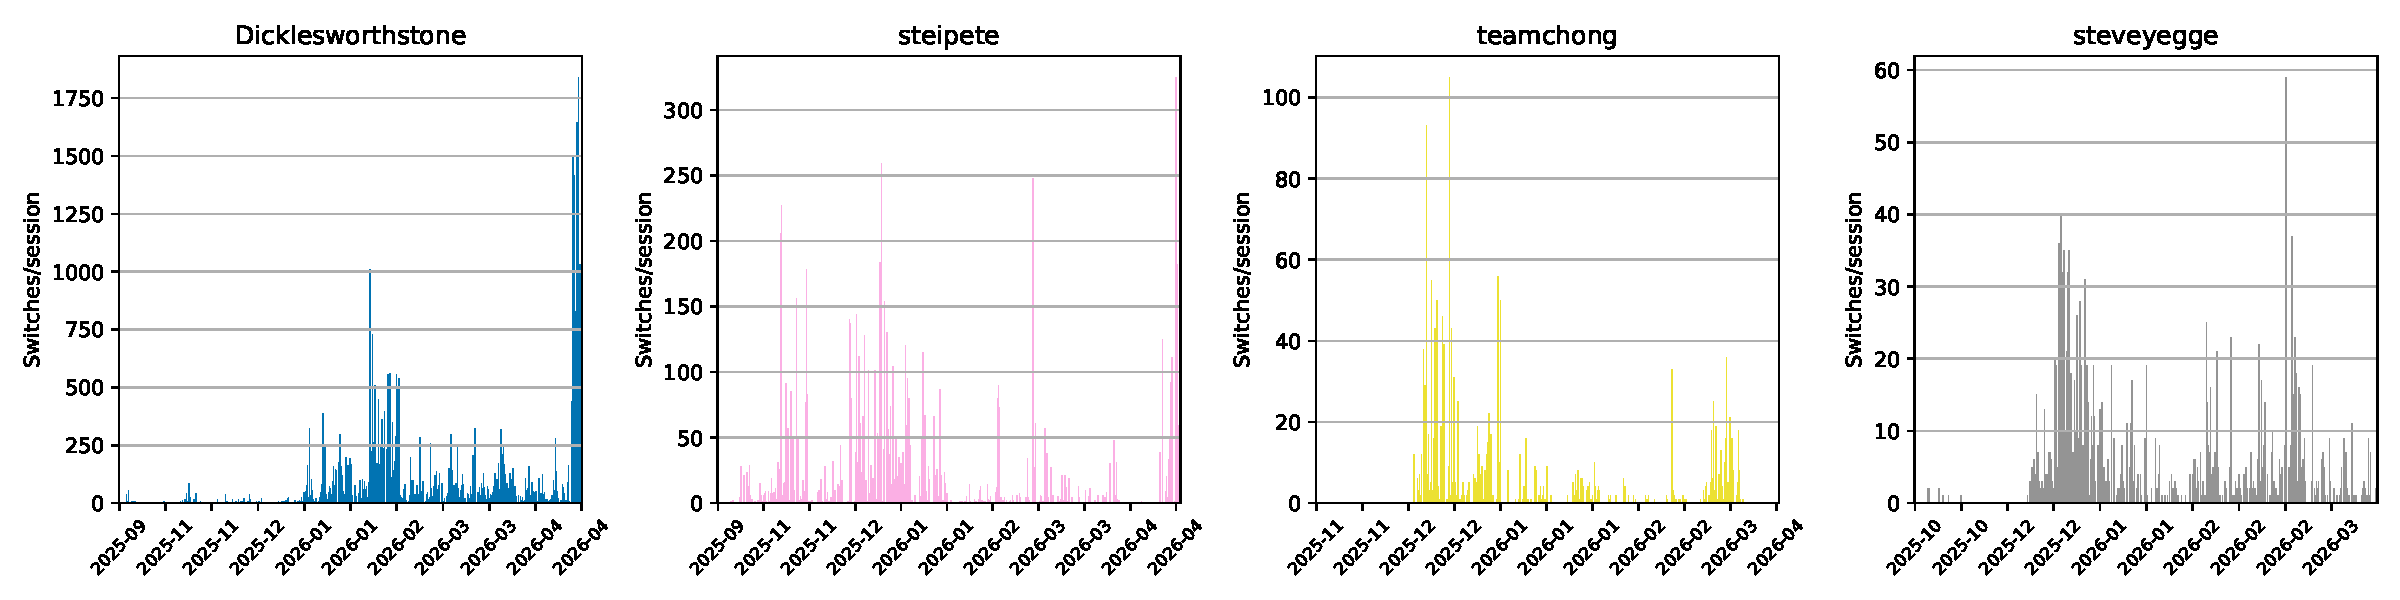
\includegraphics[width=\linewidth]{../data/exports-RQ4/plots/switches_session_four_devs_row.pdf}
    \caption{Repository switches per session.}
    \label{fig:rq4-switches-session-four}
  \end{subfigure}
  \caption{Repository switching behavior (RQ3) of four representative developers (Dicklesworthstone, steipete, teamchong, steveyegge).}
  \label{fig:rq4-four-devs}
\end{figure*}


\subsection{RQ4: Commit Characteristics}
\label{sec:rq4-results}

\subsubsection{Commit size and breadth}

\textbf{The typical commit is focused, with extreme outliers.}
\autoref{tab:rq4-churn-scattering} and \autoref{tab:rq4-breadth} report the per-commit distributions.
The median commit changes 27 (philipp-spiess) to 88 (Dicklesworthstone) lines,
touches one file for ruvnet and two for every other developer, and spans one
top-level directory.
Between 76.4\% (ruvnet) and 89.0\% (steveyegge) of commits stay within five files, and commits spanning more than one top-level directory are a minority, from 15.3\% (clubanderson) to 41.3\% (obra).
These medians describe compact changes, while the p95 and maximum values show
that every developer also produces much broader commits.

\begin{table}[tb]
  \caption{Per-commit churn and changed files distributions by developer.}
    \label{tab:rq4-churn-scattering}
  \centering
  \scriptsize
  \setlength{\tabcolsep}{3.2pt}
  \begin{tabular}{llrrrrrrrr}
    \toprule
    Developer & Metric & Min & P5 & P25 & Median & Mean & P75 & P95 & Max \\
    \midrule
    \multirow{2}{*}{Aggregate} & Churn & 0 & 2 & 13 & 70 & 1,116.2 & 263 & 1,610 & 6,855,492 \\
    & Files & 0 & 1 & 1 & 2 & 7.1 & 4 & 14 & 20,241 \\
    \addlinespace
    \multirow{2}{*}{steipete} & Churn & 0 & 2 & 11 & 50 & 493.9 & 165 & 899 & 2,382,134 \\
    & Files & 0 & 1 & 1 & 2 & 7.6 & 5 & 17 & 20,241 \\
    \addlinespace
    \multirow{2}{*}{Dicklesworthstone} & Churn & 0 & 2 & 14 & 88 & 964.2 & 346 & 1,771.9 & 6,855,492 \\
    & Files & 0 & 1 & 1 & 2 & 5.7 & 3 & 12 & 17,647 \\
    \addlinespace
    \multirow{2}{*}{ruvnet} & Churn & 0 & 2 & 6 & 46 & 8,833.8 & 501.5 & 13,768.8 & 5,418,284 \\
    & Files & 0 & 1 & 1 & 1 & 27.5 & 5 & 55 & 9,675 \\
    \addlinespace
    \multirow{2}{*}{obra} & Churn & 0 & 3 & 23 & 81 & 469.4 & 219 & 982.2 & 141,424 \\
    & Files & 0 & 1 & 1 & 2 & 5.0 & 4 & 11 & 871 \\
    \addlinespace
    \multirow{2}{*}{philipp-spiess} & Churn & 0 & 2 & 5 & 27 & 279.7 & 159.2 & 1,312.8 & 23,037 \\
    & Files & 0 & 1 & 1 & 2 & 3.6 & 3 & 12 & 132 \\
    \addlinespace
    \multirow{2}{*}{mavam} & Churn & 0 & 2 & 10 & 36 & 642.9 & 147 & 1,128.6 & 613,247 \\
    & Files & 0 & 1 & 1 & 2 & 10.4 & 4 & 20 & 2,732 \\
    \addlinespace
    \multirow{2}{*}{teamchong} & Churn & 0 & 3 & 21 & 82 & 1,170.9 & 313 & 2,388.0 & 462,470 \\
    & Files & 0 & 1 & 1 & 2 & 6.5 & 5 & 16 & 1,469 \\
    \addlinespace
    \multirow{2}{*}{clubanderson} & Churn & 0 & 2 & 16 & 68 & 1,299.7 & 147 & 1,123 & 3,925,715 \\
    & Files & 0 & 1 & 1 & 2 & 9.2 & 4 & 14 & 19,664 \\
    \addlinespace
    \multirow{2}{*}{steveyegge} & Churn & 0 & 2 & 11 & 63 & 440.8 & 244 & 1,608.6 & 66,836 \\
    & Files & 0 & 1 & 1 & 2 & 3.3 & 3 & 10 & 259 \\
    \bottomrule
  \end{tabular}
\end{table}

\textbf{Busy days contain more commits, not consistently larger commits.} The developers are
active on 73 to 176 of the 181 observation days, with a
median of 7 (philipp-spiess) to 304 (Dicklesworthstone) commits per active day,
accumulating a median of 1,596 to 147,294 changed lines per active day.
Across developers, the Spearman correlation between commits per day and total
daily churn ranges from 0.53 to 0.86, whereas the correlation with median
per-commit churn ranges only from -0.41 to 0.24. High output is therefore
associated mainly with producing more commits.

\textbf{Agent-attributed commits tend to be larger.}
Attributed commits have a median churn of 98 lines against 53 for
unattributed ones. Two developers are on the opposite side:~ruvnet with
40 against 243 lines and clubanderson with 52 against 72, which shows that the
relation is a property of individual workflows rather than of agent use as such.

\textbf{ruvnet combines the narrowest typical commit with the heaviest tail.}
Its median commit touches a single file, the lowest value of the cohort, while
its p95 reaches 55 files and 13,769 changed lines, against at most 20 files and
2,388 lines for every other developer. Its output alternates between minimal
edits and occasional sweeping changes, a pattern that no other
developer in the cohort exhibits.

\begin{table}[tb]
  \caption{Commit breadth and daily volume by developer. Focused commits touch at most
    five files and scattered commits touch more than ten.}
  \label{tab:rq4-breadth}
  \centering
  \scriptsize
  \setlength{\tabcolsep}{2.4pt}
  \begin{tabular}{lrrrrrrrrrrr}
    \toprule
    & & \multicolumn{2}{c}{Files} & \multicolumn{3}{c}{Top-level dir.} & \multicolumn{2}{c}{Commits (\%)} & \multicolumn{3}{c}{Daily activity} \\
    \cmidrule(lr){3-4}\cmidrule(lr){5-7}\cmidrule(lr){8-9}\cmidrule(lr){10-12}
    Developer & Commits & Med. & P95 & Med. & Mean & $>$1 (\%) & Focused & Scattered & Days & Com./day & Churn/day \\
    \midrule
    steipete & 35,089 & 2 & 17 & 1 & 1.56 & 35.0 & 78.0 & 10.0 & 173 & 188 & 41,624 \\
    Dicklesworthstone & 70,843 & 2 & 12 & 1 & 1.44 & 30.8 & 86.1 & 6.2 & 176 & 304 & 147,294 \\
    ruvnet & 5,383 & 1 & 55 & 1 & 1.51 & 24.2 & 76.4 & 13.9 & 141 & 15 & 53,654 \\
    obra & 4,419 & 2 & 11 & 1 & 1.60 & 41.3 & 84.0 & 5.7 & 144 & 20 & 4,091 \\
    philipp-spiess & 808 & 2 & 12 & 1 & 1.33 & 23.5 & 84.3 & 6.3 & 73 & 7 & 1,596 \\
    mavam & 2,685 & 2 & 20 & 1 & 1.57 & 33.5 & 80.0 & 10.9 & 152 & 13 & 3,084 \\
    teamchong & 7,204 & 2 & 16 & 1 & 1.47 & 30.6 & 79.8 & 8.7 & 141 & 31 & 22,408 \\
    clubanderson & 8,536 & 2 & 14 & 1 & 1.20 & 15.3 & 83.6 & 7.3 & 143 & 46 & 12,283 \\
    steveyegge & 9,029 & 2 & 10 & 1 & 1.26 & 16.2 & 89.0 & 4.4 & 129 & 46 & 12,096 \\
    \bottomrule
  \end{tabular}
\end{table}

\subsubsection{Evolution over time}

\textbf{Commit-size trajectories differ across developers.}
\autoref{fig:rq4-churn-evolution} and \autoref{fig:rq4-scattering-evolution}
show the daily distributions of both measures. From November to April, median churn rises from
20 to 60 lines for steipete, 6 to 54 for clubanderson, 66 to 104 for obra, and
39 to 62 for mavam. It falls from 410 to 194.5 for ruvnet, 150 to 100 for
teamchong, and 84 to 51 for steveyegge. There is no common monotonic trend:
some workflows move toward larger typical commits, others toward smaller ones,
and others remain comparatively stable.

\textbf{Daily variation is often episodic.} On short periods or isolated days, the median rises by an order of magnitude, such as
steveyegge in early December 2025 and mavam in late March 2026. These episodes correspond to bursts of
bulk changes and dissipate within days. The onset of agent-assisted activity is equally visible, most clearly for
philipp-spiess, whose commits begin in January 2026 and immediately settle at the
same per-commit scale as the rest of the cohort.

\begin{figure}[tb]
  \centering
  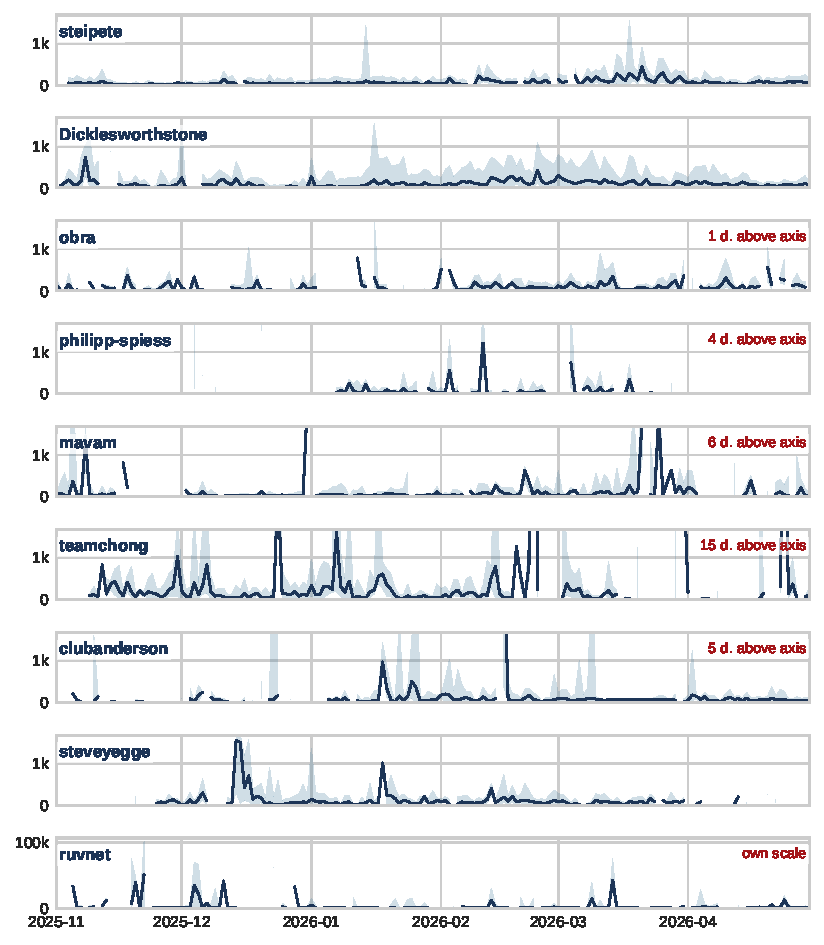
\includegraphics[width=\linewidth]{figures/rq4/churn-evolution}
  \caption{Daily per-commit Git churn by developer, in changed lines per commit.
    The line is the daily median and the band spans p25 to p75 of that day's
    commits. The eight upper panels share one time axis and Y range, which
    covers the bulk of their daily values so that a handful of days runs above
    it; ruvnet is shown on its own, wider scale.}
  \label{fig:rq4-churn-evolution}
\end{figure}

\begin{figure}[tb]
  \centering
  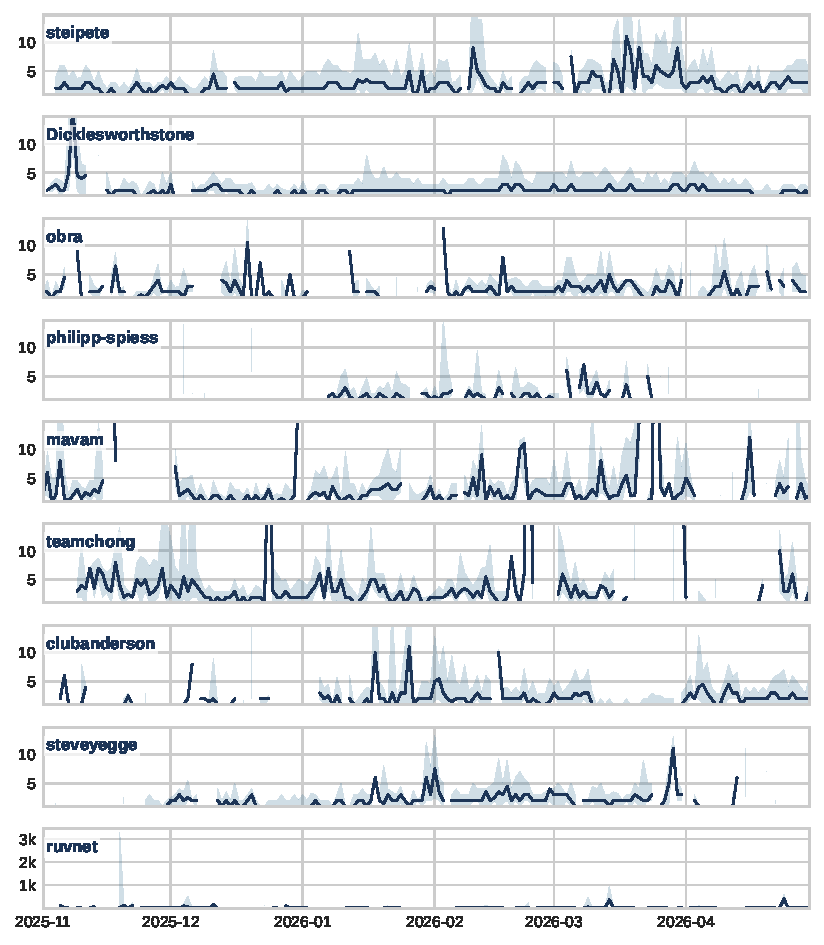
\includegraphics[width=\linewidth]{figures/rq4/scattering-evolution}
  \caption{Daily per-commit file scattering by developer, in files touched per
    commit, presented as in \autoref{fig:rq4-churn-evolution}.}
  \label{fig:rq4-scattering-evolution}
\end{figure}

\subsubsection{What the commits touch}

\textbf{Less than a third of the churn is code.}
\autoref{fig:rq4-commit-categories} shows the distribution of churn per file type and per developer. Across
the cohort, code accounts for 30.7\% of the churn, tests for 15.4\%,
documentation for 12.1\%, data for 7.3\%, and configuration for 6.4\%, while
28.2\% falls in the residual \emph{others} category. We do not infer a common
provenance for that residual category. Its largest-churn files nevertheless
provide useful qualitative examples: a vendored test matrix and an
agent-maintained memory store for ruvnet account for 3.0 and 1.7 million changed
lines across three changes each, while a bundled WebChat JavaScript file for
steipete accounts for 0.5 million changed lines across 42 changes. The
composition varies widely between developers.
Code ranges from 10.9\% (clubanderson) to 47.2\% (philipp-spiess) of churn.
Documentation reaches 35.0\% for steipete and 30.0\% for mavam, configuration
43.4\% for mavam and 38.1\% for philipp-spiess, and data 45.9\% for steveyegge.
The residual category accounts for 74.1\% of clubanderson's churn and 45.2\%
of ruvnet's.

\begin{figure}[tb]
  \centering
  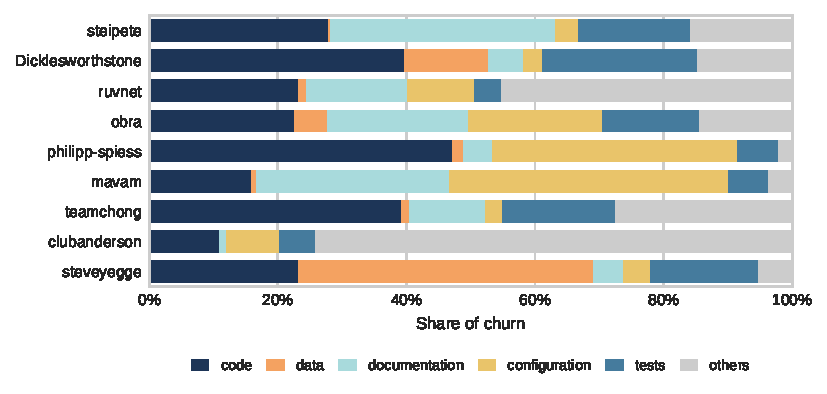
\includegraphics[width=\linewidth]{figures/rq4/commit-categories}
  \caption{Share of each developer's churn by the kind of file it changes. Each
    changed file is assigned to exactly one category from its path and
    extension; \emph{others} is the residual category.}
  \label{fig:rq4-commit-categories}
\end{figure}

\subsubsection{Revisits and rework}

\textbf{Most changes revisit recently written code.}
\autoref{tab:rq4-rework} reports the result. Between 50.8\% (mavam) and 88.1\%
(steveyegge) of all file changes revisit a file the developer had already
changed, and between 41.3\% and 76.8\% do so within seven days of the previous
change. Same-day revisits alone account for 23.9\% to 42.5\% of changes, and a
file receives 2.03 (mavam) to 8.42 (steveyegge) changes over the window. The
cohort concentrates its output on code it has just written rather than spreading
it across an ever-widening surface, which is consistent with a workflow of rapid
iteration in which an agent proposes a change, the result is exercised, and the
same file is amended shortly afterwards.

\textbf{Part of the recorded activity is agents maintaining their own state.}
Three developers commit substantial volumes of agent-maintained files, such as
in-repository issue trackers, agent memory, and agent instructions. For
steveyegge these files account for 15.4\% of file changes and 51.7\% of total
churn, for ruvnet 12.5\% and 16.4\%, and for Dicklesworthstone 8.6\% and 10.1\%;
they stay below 2\% for the remaining six developers. Agentic workflows thus
write their own coordination state into the repository, which inflates the
recorded activity of the developers who adopt them.

\begin{table}[tb]
  \caption{File revisit statistics by developer. A revisit is a change to a file
    the same developer had already changed earlier in the window, in the same
    repository.}
  \label{tab:rq4-rework}
  \centering
  \scriptsize
  \setlength{\tabcolsep}{4pt}
  \begin{tabular}{lrrrrrr}
    \toprule
    Developer & File changes & Distinct files & Changes/file & Revisits (\%) & $\leq$7 days (\%) & Same day (\%) \\
    \midrule
    steipete & 306,352 & 92,041 & 3.33 & 70.0 & 60.2 & 41.4 \\
    Dicklesworthstone & 401,553 & 147,506 & 2.72 & 63.3 & 51.9 & 34.5 \\
    ruvnet & 148,263 & 66,498 & 2.23 & 55.1 & 47.0 & 34.4 \\
    obra & 22,189 & 6,705 & 3.31 & 69.8 & 62.5 & 42.5 \\
    philipp-spiess & 2,943 & 1,034 & 2.85 & 64.9 & 56.2 & 28.4 \\
    mavam & 27,807 & 13,675 & 2.03 & 50.8 & 41.3 & 23.9 \\
    teamchong & 46,482 & 14,754 & 3.15 & 68.3 & 61.4 & 36.2 \\
    clubanderson & 78,906 & 31,363 & 2.52 & 60.3 & 54.1 & 40.2 \\
    steveyegge & 30,055 & 3,570 & 8.42 & 88.1 & 76.8 & 42.0 \\
    \bottomrule
  \end{tabular}
\end{table}

\begin{table}[tb]
  \caption{Agent attribution by developer. Attributed is the share of commits
    carrying any harness signal; Author/msg.\ the share carrying an author,
    co-author, or message signal. The remaining columns report the number of
    commits of each kind with their median churn and median changed files.}
  \label{tab:rq4-attribution}
  \centering
  \scriptsize
  \setlength{\tabcolsep}{3.2pt}
  \begin{tabular}{lrrrrrrrrr}
    \toprule
    & & \multicolumn{2}{c}{Signal (\%)} & \multicolumn{3}{c}{Agent-attributed} & \multicolumn{3}{c}{Unattributed} \\
    \cmidrule(lr){3-4}\cmidrule(lr){5-7}\cmidrule(lr){8-10}
    Developer & Commits & Attributed & Author/msg. & Commits & Churn & Files & Commits & Churn & Files \\
    \midrule
    \textbf{Aggregate} & 143,996 & 48.3 & 47.1 & 69,533 & 98 & 2 & 74,463 & 53 & 2 \\
    steipete & 35,089 & 2.8 & 0.0 & 981 & 63 & 3 & 34,108 & 50 & 2 \\
    Dicklesworthstone & 70,843 & 75.0 & 74.8 & 53,120 & 112 & 2 & 17,723 & 45 & 1 \\
    ruvnet & 5,383 & 88.8 & 87.5 & 4,782 & 40 & 1 & 601 & 243 & 3 \\
    obra & 4,419 & 49.4 & 47.7 & 2,184 & 86.5 & 2 & 2,235 & 75 & 2 \\
    philipp-spiess & 808 & 4.1 & 0.2 & 33 & 64 & 2 & 775 & 27 & 2 \\
    mavam & 2,685 & 44.3 & 36.3 & 1,190 & 34 & 2 & 1,495 & 37 & 2 \\
    teamchong & 7,204 & 0.7 & 0.5 & 48 & 145 & 4 & 7,156 & 81 & 2 \\
    clubanderson & 8,536 & 28.4 & 27.5 & 2,428 & 52 & 2 & 6,108 & 72 & 1 \\
    steveyegge & 9,029 & 52.8 & 52.1 & 4,767 & 88 & 2 & 4,262 & 32 & 1 \\
    \bottomrule
  \end{tabular}
\end{table}

%-----------------------------------------------------------------------
\section{Discussion}
\label{sec:discussion}

\subsection{Threats to Validity}
\begin{itemize}
  \item \emph{Construct}: agent harness detection relies on co-author trailers and message patterns; developers who suppress signals (steipete) are undercounted, interviews aren't guaranteed to reveal actual developer behavior.
  \item \emph{Internal}: selection bias --- curated cohort; not a random sample; findings may not generalise. changes in frequency or behavior could be driven by external factors
  \item \emph{External}: seven developers, one six-month window; early-adoption period; behaviors may differ post-2026.
  \item \emph{Reliability}: GitHub API rate limits forced sampling on high-volume developers; daily totals may undercount.
\end{itemize}

%-----------------------------------------------------------------------
\section{Conclusion}
\label{sec:conclusion}

\begin{itemize}
  \item We present the first commit-level longitudinal study of hyperactive AI-augmented developers on GitHub.
  \item Commit activity rises sharply and then declines for most developers, while repository breadth and detected harness signals vary substantially across the cohort.
  \item The curated dataset and analysis scripts are released to enable replication and extension.
  \item Future work: expand cohort (candidate developers under evaluation), extend observation window, compare against matched non-AI developer baselines.
\end{itemize}

%-----------------------------------------------------------------------
\bibliographystyle{spbasic}
\bibliography{references}

\appendix


\end{document}
